\documentclass{article}
\usepackage{amsmath,amsthm,amsfonts,amssymb,fullpage,graphicx}

\begin{document}

\begin{flushright}
Kris Harper

MATH 16300

Mikl\'{o}s Ab\'{e}rt

May 27, 2008
\end{flushright}

\begin{flushleft}

\Large

Sheet 14: Cauchy Sequences\newline

\normalsize

\textbf{Definition 1 (Cauchy Sequence)}
\textsl{We say that a sequence $(a_n)$ is a Cauchy sequence if for each $\varepsilon > 0$ there exists $N \in \mathbb{N}$ such that if $n,m \geq N$, then $|a_n-a_m| < \varepsilon$.}\newline

\textbf{Lemma 2}
\textsl{Every convergent sequence has the Cauchy property.}
\begin{proof}
Let $(a_n)$ converge to $a$ and let $\varepsilon > 0$. Consider $\varepsilon/2$. Then there exists $N \in \mathbb{N}$ such that for all $n>N$ we have $a_n \in (a - \varepsilon/2 ; a + \varepsilon/2)$. But then also for all $m,n > N$ we have $a_m, a_n \in (a - \varepsilon/2 ; a + \varepsilon/2)$. Then the distance between $a_m$ and $a_n$ is no more than $\varepsilon / 2 + \varepsilon /2 = \varepsilon$. Thus, there exists $N \in \mathbb{N}$ such that for all $m,n > N$ we have $|a_m-a_n| < \varepsilon$.
\end{proof}

\textbf{Lemma 3}
\textsl{Let $(a_n)$ be a Cauchy sequence and let $(b_k = a_{n_k})$ be a subsequence. If $(b_k)$ converges then so does $(a_n)$.}
\begin{proof}
Let $(b_k = a_{n_k})$ be a subsequence of $(a_n)$ which converges to $a$ and let $\varepsilon > 0$. Then there exists $N_1 \in \mathbb{N}$ such that for all $k > N_1$ we have $|a-b_k| < \varepsilon/2$. But also $(a_n)$ is a Cauchy sequence and so there exists some $N_2 \in \mathbb{N}$ such that for all $n,m > N_2$ we have $|a_m - a_n| < \varepsilon/2$. Let $N = \max (N_1,N_2)$. Then for all $n,m > N$ we have $|a-b_n| < \varepsilon/2$ and $|a_m - a_n| < \varepsilon/2$. Now choose $n>N$ such that $a_n = b_n$. Then for all $m > n > N$ we have $|a-a_n| < \varepsilon/2$ and $|a_m - a_n| < \varepsilon/2$. Thus by the triangle inequality for all $m>n>N$ we have $|a - a_m| \leq |a - a_n| + |a_n - a_m| < \varepsilon$ and so $(a_n)$ converges to $a$.
\end{proof}

\textbf{Lemma 4}
\textsl{Every Cauchy sequence is bounded.}
\begin{proof}
Let $(a_n)$ be a Cauchy sequence and let $\varepsilon > 0$. There exists $N \in \mathbb{N}$ such that for all $n > N$ we have $|a_N - a_n| < \varepsilon$. Then there are finitely many $n \in \mathbb{N}$ such that $a_n \notin (-\varepsilon + a_N ; \varepsilon + a_N)$. Then the largest of these $a_n$ is greater than or equal to every other term of $(a_n)$. Note that if there are no terms of $(a_n)$ greater than $a_N + \varepsilon$, then we can choose a smaller epsilon so that such a term exists. A similar argument shows that there is a lower bound of $(a_n)$.
\end{proof}

\textbf{Theorem 5}
\textsl{A sequence is convergent if and only if it is Cauchy.}
\begin{proof}
Let $(a_n)$ be a Cauchy sequence. Then by Lemma 4 we know $(a_n)$ is bounded and therefore there exists a convergent subsequence of $(a_n)$ (13.16, 14.4). But then by Lemma 3 we know $(a_n)$ converges (14.3). Conversely if a sequence is convergent then it Cauchy by Lemma 2 (14.2).
\end{proof}

\textbf{Definition 6}
\textsl{Let $(a_n)$ be a bounded sequence and $A$ be the set of its accumulation points. We define its limes inferior, $\lim \inf_{n \rightarrow \infty} a_n$, to be the first point of $A$ and the limes superior, $\lim \sup_{n \rightarrow \infty} a_n$, to be the last point of $A$.}\newline

\textbf{Corollary 7}
\textsl{Let $(a_n)$ be a bounded sequence. Then $\lim \inf_{n \rightarrow \infty} a_n \leq 
\lim \sup_{n \rightarrow \infty} a_n$ and equality holds if and only if the sequence is convergent.}
\begin{proof}
Let $A$ be the set of accumulation points for $(a_n)$. Since $\lim \inf_{n \rightarrow \infty} a_n$ is the first point of $A$, we have $\lim \inf_{n \rightarrow \infty} a_n \leq a$ for all $a \in A$. But since $\lim \sup_{n \rightarrow \infty} a_n \in A$ we have $\lim \inf_{n \rightarrow \infty} a_n \leq \lim \sup_{n \rightarrow \infty} a_n$. Suppose now that $\lim \inf_{n \rightarrow \infty} a_n = \lim \sup_{n \rightarrow \infty} a_n$. Then the first and last points of $A$ are equal and so $A$ only has one accumulation point. But then since $(a_n)$ is bounded we have $(a_n)$ is convergent (13.17). Conversely assume that $(a_n)$ is convergent. Then $(a_n)$ only has one accumulation point and so $A$ contains one point (13.17). But then $\lim \inf_{n \rightarrow \infty} a_n = \lim \sup_{n \rightarrow \infty} a_n$.
\end{proof}

\textbf{Theorem 8}
\textsl{Let $(a_n)$ be a bounded sequence. Then
\[
\lim \inf_{n \rightarrow \infty} a_n = \lim_{n \rightarrow \infty} (\inf \{a_k \mid k > n\})
\]
and
\[
\lim \sup_{n \rightarrow \infty} a_n = \lim_{n \rightarrow \infty} (\sup \{a_k \mid k > n\}).
\]}
\begin{proof}
Consider the sequence $(b_n)$ where $b_n = \inf \{a_k \mid k > n\}$. Then $(b_n)$ is bounded because $(a_n)$ is bounded and it's increasing because each infimum will either be less than or equal to the previous one. Thus $\lim_{n \rightarrow \infty} b_n = \sup \{b_n \mid n \in \mathbb{N}\} = s$ (13.18). Now consider some region $(p;q)$ with $s \in (p;q)$. Note that $p < \inf \{a_k \mid k > n\} = r$ for some $n$, otherwise there would exist some point in $(p;s)$ which would be an upper bound for $\{b_n \mid n \in \mathbb{N}\}$. Note that there are finitely many $n$ such that $a_n < r$ because of how $r$ is defined. Thus there are finitely many $n$ with $a_n < p$. But also there must be finitely many $n$ with $a_n > q$ because if there were infinitely many then there would exist $a_k > q$ such that $k$ is greater than every index of $a_n \leq q$. But this contradicts how $s$ is defined. Thus there are infinitely many $n$ with $a_n \in (p;q)$ and so $s$ is an accumulation point of $(a_n)$. But there can't be an accumulation point of $(a_n)$ less than $s$ because for each term or $(b_n)$ there are finitely many $n$ with $a_n$ less that it and an accumulation point would imply infinitely many such $n$. Thus $s = \lim \inf_{n \rightarrow \infty} a_n$. A similar proof holds to show $\lim \sup_{n \rightarrow \infty} a_n = \lim_{n \rightarrow \infty} (\sup \{a_k \mid k > n\})$.
\end{proof}

\textbf{Theorem 9}
\textsl{Let $(a_n)$ be a bounded sequence. Then
\[
\lim \inf_{n \rightarrow \infty} a_n = \sup \{x \mid \text{ there are finitely many $n$ with $a_n \in (-\infty ; x)$} \}
\]
and
\[
\lim \sup_{n \rightarrow \infty} a_n = \inf \{x \mid \text{ there are finitely many $n$ with $a_n \in (x ; \infty)$} \}
\]}
\begin{proof}
Let $S = \{x \mid \text{ there are finitely many $n$ with $a_n \in (-\infty ; x)$} \}$. Note that $S$ is nonempty because $(a_n)$ is bounded. Thus a lower bound for $(a_n)$ shows that $S$ is nonempty and an upper bound for $(a_n)$ shows that $S$ is bounded. Thus $\sup S = t$ exists. Let $(b_n)$ be defined such that $b_n = \inf \{a_k \mid k > n\}$ and let $s = \lim_{n \rightarrow \infty} b_n = \sup \{b_n \mid n \in \mathbb{N}\}$ (13.18, 14,8). First suppose that $t > s$. Then there exists $x \in (s;t)$ such that there are finitely many $n$ with $a_n < x$. But then if we take the largest index, $i$, of all such $a_n$ we have $\inf \{a_k \mid k > i\} > s$ which is a contradiction. So $t \leq s$. Suppose that $t < s$. Then for all $x \in (t;s)$ there are infinitely many $n$ with $a_n < x$. But this implies that there are infinitely many $n$ with $a_n \in (t;s)$ because there exists $x < t$ such that there are finitely many $n$ with $a_n < x$. But then there exists some element of $b_n$ which is less than $s$, but greater than infinitely many terms of $(a_n)$. This cannot happen and so $s=t$. But then using Theorem 8 we have $t = \lim \inf_{n \rightarrow \infty} a_n$ (14.8).
\end{proof}

\end{flushleft}

\newpage

\begin{flushright}
Kris Harper

MATH 16300

Mikl\'{o}s Ab\'{e}rt

May 27, 2008
\end{flushright}

\begin{flushleft}

\Large

Sheet 15: Series\newline

\normalsize

\textbf{Definition 1}
\textsl{A series of real numbers is an expression $\sum_{n=1}^{\infty} a_n$, where $(a_n)$ is a real sequence.}\newline

\textbf{Definition 2 (Convergent Series)}
\textsl{Let $\sum_{n=1}^{\infty} a_n$ be a series. The sequence of partial sums is defined as
\[
s_n = a_1 + a_2 + \dots + a_n = \sum_{i=1}^{n} a_i.
\]
We say that the series $\sum_{n=1}^{\infty} a_n$ converges to $s$ (or $\sum_{n=1}^{\infty} a_n = s$) if $\lim_{n \rightarrow \infty} s_n = s$. If such an $s$ exists, we say that $\sum_{n=1}^{\infty} a_n$ is convergent, otherwise it is divergent.}\newline

\textbf{Exercise 3}
\textsl{Reformulate convergence using the Cauchy property.}\newline

We say a series $\sum_{n=1}^{\infty} a_n$ is convergent if for all $\varepsilon > 0$ there exists $N \in \mathbb{N}$ such that for all $n, m > N$ we have $|s_n - s_m| < \varepsilon$.\newline

\textbf{Lemma 4}
\textsl{If $\sum_{n=1}^{\infty} a_n$ is a convergent series, the the sequence $(a_n)$ converges to $0$.}
\begin{proof}
Let $\sum_{n=1}^{\infty} a_n = s$. Then the sequence of partial sums $(s_n)$ converges to $s$ and $(s_n)$ is a Cauchy sequence. Thus for all $\varepsilon > 0$ there exists $N \in \mathbb{N}$ such that for all $n,m > N$ we have $|s_n - s_m| < \varepsilon$. But note that $s_{n+1} - s_n= a_n$ so for $n > N+1$ we have $|a_n| < \varepsilon$ which means $\lim_{n \rightarrow \infty} a_n = 0$.
\end{proof}

\textbf{Lemma 5}
\textsl{Let $\sum_{n=1}^{\infty} a_n$ be convergent with a partial sum sequence $(s_n)$. Let $n_0 = 0$ and $n_1 < n_2 < \dots$ be a sequence of natural numbers. For $k \in \mathbb{N}$ let
\[
b_k = a_{n_{k-1}+1} + \dots + a_{n_k} = \sum_{i = n_{k-1} + 1}^{n_k} a_i.
\]
Then
\[
\sum_{k=1}^{\infty} b_k = \sum_{n=1}^{\infty} a_n.
\]}
\begin{proof}
Let $s_{b_k} = \sum_{i=1}^{k} b_i$ and $s_{a_n} = \sum_{i=1}^{n} a_i$. Then note that
\[
s_{b_k} = \sum_{i=1}^{k} b_i = \sum_{i=1}^{n_1} a_i + \sum_{i = n_{1} + 1}^{n_2} a_i + \dots + \sum_{i = n_{k-1} + 1}^{n_k} a_i = s_{a_{n_k}}.
\]
We know $\sum_{n=1}^{\infty} a_n$ is convergent so $(s_{a_n})$ converges. Also $(s_{a_{n_k}})$ is a subsequence of $(s_{a_n})$ so it converges as well (13.12). But $(s_{b_k}) = (s_{a_{n_k}})$ so $\lim_{k \rightarrow \infty} s_{b_k} = \lim_{k \rightarrow \infty} s_{a_{n_k}}$ which implies
\[
\sum_{k=1}^{\infty} b_k = \sum_{n=1}^{\infty} a_n.
\]
\end{proof}

\textbf{Theorem 6 (Geometric Series)}
\textsl{For all $t < |1|$, we have
\[
\sum_{n=0}^{\infty} t^n = \frac{1}{1-t}.
\]}
\begin{proof}
Consider a partial sum of $\sum_{n=0}^{\infty} t^n$,
\[
s_k = \sum_{n=0}^{k} t^n= 1+t+\dots+t^k = \frac{1-t^{k+1}}{1-t} = \frac{1}{1-t} - \frac{t^k}{1-t}.
\]
But since $t < |1|$ we have $\lim_{k \rightarrow \infty} t^k/(1-t) = 0$. So then $\lim_{k \rightarrow \infty} s_k = 1/(1-t) + 0$ which means
\[
\sum_{n=0}^{\infty} t^n = \frac{1}{1-t}.
\]
\end{proof}

\textbf{Theorem 7}
\textsl{The series $\sum_{n=1}^{\infty} 1/n$ is not convergent.}
\begin{proof}
Suppose that $\sum_{n=1}^{\infty} 1/n$ is convergent. Create a sequence $(b_k)$ as in Lemma 5 such that
\[
b_k = \sum_{i = n_{k-1} + 1}^{n_k} \frac{1}{n}
\]
where $n_k = 2^{k-1}$ for $k \in \mathbb{N}$ and $n_0 = 0$. Note that for $k \geq 2$, $b_k$ has $2^{k-1} - 2^{k-2} = 2^{k-2}$ terms, the smallest of which is $1/2^{k-1}$. Thus, for all $k \geq 2$, $b_k \geq 2^{k-2}/2^{k-1} = 1/2$. Also $b_1 = \sum_{n=1}^{1} 1/n = 1$. So for all $k \in \mathbb{N}$ we have $b_k \geq 1/2$. But then there are infinitely many $k \in \mathbb{N}$ such that $b_k \notin (-1/2 ; 1/2)$ so $\lim_{k \rightarrow \infty} b_k \neq 0$. Thus, $\sum_{k=1}^{\infty} b_k$ is not convergent (15.4). But we know that $\sum_{k=1}^{\infty} b_k = \sum_{n=1}^{\infty} a_n$ which is a contradiction (15.5). Thus $\sum_{n=1}^{\infty} 1/n$ is not convergent.
\end{proof}

\textbf{Theorem 8 (Alternating Sign Series)}
\textsl{Let $\sum_{n=1}^{\infty} a_n$ be a series with the following properties:
1) $a_n$ is positive if $n$ is odd and negative if $n$ is even;
2) $|a_{n+1}| < |a_n|$ for all $n$;
3) $\lim_{n \rightarrow \infty} a_n = 0$.
Then $\sum_{n=1}^{\infty} a_n$ is convergent.}
\begin{proof}
Let $\varepsilon > 0$. Then there exists $N \in \mathbb{N}$ such that for all $n > N$ we have $|a_n| < \varepsilon$. Let $n \in \mathbb{N}$ such that $n > N$ and $n$ is even. Then $a_{n+1} > 0$. We have $s_{n+1} = s_{n} + a_{n+1} > s_{n}$. Also $a_{n+2} < 0$ and $|a_{n+2}| < |a_{n+1}|$ so $a_{n+1} + a_{n+2} > 0$. Then $s_{n+1} > s_{n+1} + a_{n+2} = s_{n+2} = s_{n} + a_{n+1} + a_{n+2} > s_{n}$. So for $n > N$ even we have $s_{n} \leq s_{n+2} \leq s_{n+1}$ and a similar proof shows that for $n > N$ odd we have $s_{n} \geq s_{n+2} \geq s_{n+1}$. Use strong induction on $n$ to show that for $k + N$ even $s_{N} \leq s_{k+N} \leq s_{N+1}$. We see that for $k=1$ we have $s_N \leq s_{N+1} \leq s_{N+1}$ which is true since $a_{N+1}$ is positive.
We've also shown the case for $k=2$. Assume that for $n+N$ even we have $s_N \leq s_{N+n} \leq s_{N+1}$. Consider $s_{N+n+2}$. We know $s_{N+n} \leq s_{N+n+2} \leq s_{N+n+1}$ and $s_{N+n-1} \leq s_{N+n+1} \leq s_{N+n}$. Combining these three inequalities we have $s_N \leq s_{N+n+2} \leq s_{N+1}$. Thus for all even $N+n$ we have $s_N \leq s_{N+n} \leq s_{N+1}$. A similar proof holds to show that for odd $N+n$ we have $s_{N} \leq s_{N+n} \leq s_{N+1}$. Since this is true for any $N$ given $\varepsilon$, for any region $(s_{N};s_{N+1})$ there are finitely many $n$ with $s_n$ not in the region. Thus $\sum_{n=1}^{\infty} a_n$ is convergent.
\end{proof}

\textbf{Exercise 9}
\textsl{The series
\[
\sum_{n=1}^{\infty} \frac{(-1)^{n+1}}{n}
\]
is convergent.}
\begin{proof}
Note that for $n$ odd we have $a_n = (-1)^{n+1}/n$ and since $n+1$ is even and $n > 0$ we have $a_n = 1/n > 0$. For $n$ even $n+1$ is odd so $a_n = (-1)^{n+1}/n = -1/n < 0$. Also $|a_{n+1}| = 1/(n+1) < 1/n = |a_n|$. Finally we know that $\lim_{n \rightarrow \infty} a_n = 0$ (13.4). Since this series fulfills the requirements of Theorem 8, it must be convergent.
\end{proof}

\textbf{Definition 10}
\textsl{A series $\sum_{n=1}^{\infty} a_n$ is called absolutely convergent if the series $\sum_{n=1}^{\infty} |a_n|$ is convergent.}\newline

\textbf{Lemma 11}
\textsl{$\sum_{n=1}^{\infty} a_n$ is absolutely convergent if and only if there exists $C \in \mathbb{R}$ such that for all $N \in \mathbb{N}$, $\sum_{n=1}^{N} |a_n| \leq C$.}
\begin{proof}
Suppose that $\sum_{n=1}^{\infty} a_n$ is absolutely convergent. Let $s_k = \sum_{n=1}^{k} |a_n|$. Then $(s_n)$ is convergent and therefore bounded (13.15). Thus there exists $C \in \mathbb{R}$ such that for all $N$ we have $s_N = \sum{n=1}^{N} |a_n| \leq C$.\newline

Now suppose there exists $C \in \mathbb{R}$ such that $s_N \leq C$ for all $N$. Thus $(s_n)$ is bounded. Note that $s_n = s_{n-1} + |a_n|$ and since $|a_n| \geq 0$ for all $n$ we have $(s_n)$ is an increasing sequence. Since $(s_n)$ is bounded and increasing we know it is convergent (13.18). Thus $\sum_{n=1}^{\infty} |a_n|$ is convergent and so $\sum_{n=1}^{\infty} a_n$ is absolutely convergent.
\end{proof}

\textbf{Theorem 12 (Comparison Criterion)}
\textsl{Let $\sum_{n=1}^{\infty} a_n$ and $\sum_{n=1}^{\infty} b_n$ be two series. Suppose there is some $N$ such that for all $n \geq N$ we have $|a_n| \leq |b_n|$. Then if $\sum_{n=1}^{\infty} b_n$ is absolutely convergent so is $\sum_{n=1}^{\infty} a_n$.}
\begin{proof}
For all $M \geq N$ note that
\[
\sum_{n=N}^{M} |a_n| \leq \sum_{n=N}^{M} |b_n| \leq \sum_{n=1}^{M} \leq C
\]
for some $C \in \mathbb{R}$ because every term in $(|b_n|)$ is greater than or equal to zero (15.11). Also note that
\[
\sum_{n=1}^{M} |a_n| \leq C + \sum_{n=1}^{N-1} |a_n| \leq C'
\]
for some $C' \in \mathbb{R}$ because every term of $(|a_n|)$ is greater than or equal to zero. Also note that for $M' < N \leq M$ we have
\[
\sum_{n=1}^{M'} |a_n| \leq \sum_{n=1}^{M} \leq C'
\]
so that for all $M$ we have $\sum_{n=1}^{M} |a_n| \leq C'$. By Lemma 11 $\sum_{n=1}^{\infty} a_n$ is absolutely convergent (15.11).
\end{proof}

\textbf{Corollary 13 (Quotient Criterion)}
\textsl{Let $\sum_{n=1}^{\infty} a_n$ be a series. Suppose that there is an $N \in \mathbb{N}$ and $0<r<1$, such that $|a_{n+1}/a_n| \leq r$ for all $n \geq N$. Then $\sum_{n=1}^{\infty} a_n$ is absolutely convergent.}
\begin{proof}
Use induction on $n$ to show that $|a_{N+n}| \leq |a_N| r^n$. For the base case, $n=1$ we have $|a_{N+1}| \leq |a_N| r$ by assumption. Assume that for $n \in \mathbb{N}$ we have $|a_{N+n}| \leq |a_N| r^n$ so $|a_{N+n}| r \leq |a_N| r^{n+1}$. Then note that $|a_{N+n+1}| \leq |a_{N+n}| r \leq |a_N| r^{n+1}$ as desired. Thus for $n \geq N$ we have $|a_n| \leq |a_N| r^{n-N}$. Let $b_n = |a_N| r^{n-N}$. Then for $n>N$ we have $|a_n| \leq |a_N| r^{n-N} = |a_N r^{n-N}| = |b_n|$ since $r>0$. But also
\[
\sum_{n=1}^{\infty} |a_N r^{n-N} | = \sum_{n=0}^{\infty} |a_N| r^{n-N+1} = |a_N| r^{-N+1} \sum_{n=0}^{\infty} r^n
\]
and so $\sum_{n=1}^{\infty} b_n$ is absolutely convergent by Theorem 6, because $r>0$ and because $|a_N| r^{-N+1}$ is a constant value (15.6). Thus, by Theorem 12 we have $\sum_{n=1}^{\infty} a_n$ is absolutely convergent.
\end{proof}

\textbf{Definition 14}
\textsl{Let $\sum_{n=1}^{\infty} a_n$ be a series. A reordering of $\sum_{n=1}^{\infty} a_n$ is a series of the form $\sum_{n=1}^{\infty} b_n$, where $b_n=a_{f(n)}$ for some bijection $f \; : \; \mathbb{N} \rightarrow \mathbb{N}$.}\newline

\textbf{Lemma 15}
\textsl{Let $\sum_{n=1}^{\infty} a_n$ be an absolutely convergent series, and let $\sum_{n=1}^{\infty} b_n$ be a reordering of it. Then for every $k \in \mathbb{N}$ there exists $L \in \mathbb{N}$ such that for all $l \geq L$,
\[
\left | \sum_{n=1}^{\infty} a_n - \sum_{n=1}^{l} b_n \right | \leq \sum_{n=k+1}^{\infty} |a_n|.
\]}
\begin{proof}
Let $g \; : \; \mathbb{R} \rightarrow \mathbb{R}$ be a function such that $g(x) = |x|$. We know that since $g$ is continuous, for a sequence $(a_n)$, if $\lim_{n \rightarrow \infty} a_n = a$, then $\lim_{n \rightarrow \infty} |a_n| = |a|$ (13.7). We have $\sum_{n=1}^{\infty} a_n$ is absolutely convergent so $|\sum_{n=1}^{\infty} a_n| = \lim_{n \rightarrow \infty} |s_n|$. Then use induction on $n$ to show that $|s_n| \leq \sum_{k=1}^{n} |a_k|$. For $n=1$ we have $|s_1| = |a_1| = \sum_{k=1}^{1} |a_1|$. Assume that for $n \in \mathbb{N}$, $\sum_{k=1}^{n} |a_k| \geq |s_n|$. Then
\[
\sum_{k=1}^{n+1} |a_k| = \sum_{k=1}^{n} |a_k| + |a_{n+1}| \geq |s_n| + |a_{n+1}| \geq |s_n + a_{n+1}| = |s_{n+1}|
\]
by the triangle inequality and our inductive hypothesis (9.36). Therefore we have
\[
\left | \sum_{n=1}^{\infty} a_n \right | \leq \sum_{n=1}^{\infty} |a_n|.
\]
Let $k \in \mathbb{N}$ and consider the sets $A = \{a_n \mid n \leq k\}$ and $S = \{f(n) \mid n \leq k\}$. Let $L = \sup S$. Consider $l \geq L$ and let $B = \{b_n \mid n \leq l\}$ and $T = \{n \mid b_n \in B\}$. Finally let $C = \{a_n \mid n \notin T\}$. Make a new sequence $c_n$ where $n$ is the $n$th element of $C$. Note that by definition, $\sum_{n=1}^{\infty} c_n = \sum_{n=1}^{\infty} a_n - \sum_{n=1}^{l} b_n$. Then
\[
\left | \sum_{n=1}^{\infty} c_n \right | = \left | \sum_{n=1}^{\infty} a_n - \sum_{n=1}^{l} b_n \right | \leq \sum_{n=1}^{\infty} |c_n| \leq \sum_{k+1}^{\infty} |a_n|.
\]
The last inequality holds because $(c_n)$ is the sequence $(a_n)$, but with at least $k$ terms missing.
\end{proof}

\textbf{Theorem 16 (Abel Resummation Theorem)}
\textsl{Let $\sum_{n=1}^{\infty} a_n$ be an absolutely convergent series, and let $\sum_{n=1}^{\infty} b_n$ be a reordering of it. Then $\sum_{n=1}^{\infty} b_n$ absolutely convergent and
\[
\sum_{n=1}^{\infty} b_n = \sum_{n=1}^{\infty} a_n.
\]}
\begin{proof}
Let $k \in \mathbb{N}$ and consider the sets $A = \{a_n \mid n \leq k\}$ and $S = \{f(n) \mid n \leq k\}$ Let $L = \sup S$ and let $B = \{b_n \mid n \leq L\} \subseteq \{a_n \mid n \leq L\}$ since $L \geq k$. Then
\[
\sum_{n=1}^{L} |b_n| \leq \sum_{n=1}^{L} |a_n| \leq C
\]
for some $C \in \mathbb{R}$ (15.11). Note that $L$ is always some value greater than or equal to $k$ and so as $k$ increases, so does $L$. But also $(|b_n|)$ is an increasing sequence and so for any value $L' < L$ we have $\sum_{n=1}^{L'} |b_n| \leq \sum_{n=1}^L |b_n| \leq C$. Thus every partial sum of $\sum_{n=1}^{\infty} |b_n|$ is bounded and thus $\sum_{n=1}^{\infty} b_n$ is absolutely convergent (15.11). Now consider $\sum_{n=k+1}^{\infty} |a_n| = \sum_{n=1}^{\infty} |a_n| - \sum_{n=1}^{k} |a_n|$ (15.5). Take the limit as $k$ goes to infinity. We have
\[
\lim_{k \rightarrow \infty} \sum_{n=k+1}^{\infty} |a_n| = \lim_{k \rightarrow \infty} \left ( \sum_{n=1}^{\infty} |a_n| - \sum_{n=1}^{k} |a_n| \right ) = \sum_{n=1}^{\infty} |a_n| - \lim_{k \rightarrow \infty} s_k = 0.
\]
But then we have
\[
\lim_{l \rightarrow \infty} \left | \sum_{n=1}^{\infty} a_n - \sum_{n=1}^{l} b_n \right | = \left | \sum_{n=1}^{\infty} a_n - \sum_{n=1}^{\infty} b_n \right | \leq \lim_{n \rightarrow \infty} \sum_{n=k+1}^{\infty} |a_n| = 0 \text{ (15.15)}.
\]
Thus,
\[
\sum_{n=1}^{\infty} b_n = \sum_{n=1}^{\infty} a_n.
\]
\end{proof}

\textbf{Theorem 17}
\textsl{Let $\sum_{n=1}^{\infty} a_n$ be a convergent, but not absolutely convergent series. Then for all $c \in \mathbb{R}$ there exists a reordering $\sum_{n=1}^{\infty} b_n$ of $\sum_{n=1}^{\infty} a_n$ such that
\[
\sum_{n=1}^{\infty} b_n = c.
\]}
\begin{proof}
Let $A = \{a_n \mid n \in \mathbb{N}\}$. Then $A$ is nonempty and bounded, so $\sup A$ exists (6.11, 13.15). Suppose that for any positive term of $(a_n)$ there are infinitely many terms greater than or equal to it. Consider some term $a_k>0$ and the region $(-a_k ; a_k)$. Then there are infinitely many terms of $(a_n)$ which are not in $(-a_k ; a_k)$. But then $(a_n)$ does not converge to zero which means $\sum_{n=1}^{\infty} a_n$ is not convergent (13.4). This is a contradiction and so for all positive terms of $(a_n)$ there are finitely many terms greater than or equal to it. A similar proof holds to show that for a negative term of $(a_n)$, there are finitely many terms less than or equal to it.\newline

We have $\sum_{n=1}^{\infty} a_n = a$ for some $a \in \mathbb{R}$. Assume that $a_n = 0$ for finitely many $n$. We can order the positive elements of $(a_n)$ in decreasing order and the negative elements of $(a_n)$ in increasing order because there are finitely many positive or negative terms of $(a_n)$ greater than or less than any given term respectively. Define $(x_k)$ where $x_k$ is the $k$th positive element of $(a_n)$ and $(y_k)$ where $y_k$ is the $k$th negative element of $(a_n)$. Then for all $k \in \mathbb{N}$ we have $y_k < 0 \leq x_k$. Suppose there are finitely many negative terms of $(a_n)$. Then there exists a largest element, $j$, of $\{n \mid a_n < 0\}$ so that
\[
\sum_{k=1}^{j} y_k = q \text{ and } \sum_{k=1}^{j} |y_k| = -q
\]
for some $q \in \mathbb{R}$ because $y_k < 0$ for all $k$. Then we have
\[
\sum_{n=1}^{\infty} a_n = \sum_{k=1}^{\infty} x_k + \sum_{k=1}^{j} y_k
\]
and so
\[
\sum_{k=1}^{\infty} x_n = \sum_{k=1}^{\infty} |x_k| = a-q.
\]
This follows from Lemma 5 (15.5). But then
\[
(a-q)+q = \sum_{k=1}^{\infty} |x_k| + \sum_{k=1}^{j} |y_k| = \sum_{n=1}^{\infty} |a_n|
\]
which means $\sum_{n=1}^{\infty} a_n$ is absolutely convergent which is a contradiction. Thus there are infinitely many terms of $(y_k)$ and a similar proof shows there are infinitely many terms of $(x_k)$.\newline

Let $c \in \mathbb{R}$. Now suppose that for all $j \in \mathbb{N}$ we have $\sum_{k=1}^{j} x_k \leq c$. Since $x_k > 0$ for all $k$, we have the partial sums of $\sum_{k=1}^{\infty} x_k$ are bounded and increasing so it must converge to $x$ for some $x \in \mathbb{R}$ (13.18). Suppose that $\sum_{k=1}^{\infty} |y_k| = y$ for some $y \in \mathbb{R}$. Then $\sum_{n=1}^{\infty} |a_n| = \sum_{k=1}^{\infty} |x_k| + \sum_{k=1}^{\infty} |y_k| = x+y$ which is a contradiction (15.16). Thus $\sum_{k=1}^{\infty} y_k$ is not absolutely convergent so there exists $l \in \mathbb{N}$ such that $\sum_{k=1}^{l} |y_k| > c$ (15.11). But since $y_k < 0$ for all $k$ we have $-c < \sum_{k=1}^{l} y_k$.\newline

Now consider the sequence $(a'_n)$ where $a'_n = a_n$ if $a_n < 0$ and $0$ if $a_n \geq 0$. Then a partial sum of
\[
\sum_{n=1}^{\infty} a'_n \text{ is } s_{a'_n} = \sum_{k=1}^{n} a_k - \sum_{k=1}^{n'} x_k
\]
supposing there are $n'$ positive terms in the first $n$ terms of $(a_n)$. Then if we consider $\lim_{n \rightarrow \infty} s_{a'_n}$ we simply have $a-x$ since $n'$ will go to $\infty$ as $n$ does. Hence
\[
\sum_{n=1}^{\infty} a'_n = \sum_{k=1}^{\infty} y_k + 0 = a-x.
\]
Thus $\sum_{k=1}^{\infty} y_k$ is convergent, but we just showed that the partial sums of this series are unbounded which is a contradiction (13.15). Thus, for $c \in \mathbb{R}$ there exists $j \in \mathbb{N}$ such that $\sum_{k=1}^{j} x_k > c$. A similar proof shows that for $c \in \mathbb{R}$ there exists $j \in \mathbb{N}$ such that $\sum_{k=1}^{j} y_k < c$\newline

Define a reordering of $\sum_{n=1}^{\infty} a_n$, $\sum_{n=1}^{\infty} b_n$ where the first $n_1$ terms of $b_n$ are the least number of terms of $(x_k)$ such that $\sum_{k=1}^{n_1} x_k > c$. Then let the next $n_2$ terms be the least number of terms of $(y_k)$ such that $\sum_{k=1}^{n_1} x_k + \sum_{k=1}^{n_2} y_k < c$. Note that we can always do this because the partial sums of
\[
\sum_{k=1}^{\infty} x_k \text{ and } \sum_{k=1}^{\infty} y_k
\]
are unbounded. Then for odd $i \in \mathbb{N}$, $n_i$ is the least number of terms of $(x_k)$ such that
\[
\sum_{n=1}^{n_i} b_n = \sum_{k=1}^{n_i} x_k + \sum_{k=1}^{n_{i-1}} y_k > c
\]
and for even $i$, $n_i$ is the least number of terms of $(y_k)$ such that
\[
\sum_{n=1}^{n_i} b_n = \sum_{k=1}^{n_{i-1}} + \sum_{k=1}^{n_i} y_k < c.
\]
Let $s_k = \sum_{n=1}^{k} b_n$. Note that $s_k$ for $k$ between $n_i$ and $n_{i+1}$ for $i \in \mathbb{N}$ is between $s_{n_i}$ and $s_{n_{i+1}}$ because the terms of $b_n$ change sign at $n_i$. Consider some region $(p;q)$ such that $c \in (p;q)$. Since the least number of elements of $(y_k)$ are added to $s_{n_{i-1}}$ so that $s_{n_i} < c$, we have $|c - s_{n_i}|$ is always less than or equal to the absolute value of some element of $(y_k)$. Suppose that $p > s_{n_i}$ for an infinite number of odd $i$. Then $|c-p|$ is less than or equal to an infinite number of absolute values of terms of $(y_k)$. But then if we consider some $|y_k| > |c-p|$ there are an infinite number of $n$ such that $|y_n| > |y_k|$. This is a contradiction and so $p > s_{n_i}$ for finitely many odd $i$. But also for all $s_{n_i}$ with odd $i$ there are finitely many $s_k$ such that $i < k < i+1$ because the positive and negative partial sums are unbounded. Thus there are finitely many $n$ such that $s_n < p$. A similar proof shows that there are finitely many $n$ with $s_n > q$ so there are finitely many $n$ with $s_n \notin (p;q)$. Therefore $\lim_{n \rightarrow \infty} s_n = c$ and so
\[
\sum_{n=1}^{\infty} b_n = c.
\]
If there are infinitely many $n$ such that $a_n=0$ the change $b_n$ so that a zero term is added to each $n_i$th partial sum. This will not change the resulting series convergence.
\end{proof}

\textbf{Theorem 18}
\textsl{Show that if $\sum_{n=1}^{\infty} a_n$ is absolutely convergent, then it is convergent.}
\begin{proof}
Let $\varepsilon > 0$. Note that since $\sum_{n=1}^{\infty} |a_n|$ is convergent, the sequence of partial sums is Cauchy (14.5). Thus there exists $N$ such that for all $n,m > N$ we have
\[
\left | \sum_{i=1}^n a_i - \sum_{i=1}^m a_i \right | = \left | \sum_{i=m}^n a_i \right | \leq \left | \sum_{i=m}^n |a_i| \right | = \left | \sum_{i=1}^n |a_i| - \sum_{i=1}^m |a_i| \right | < \varepsilon.
\]
Thus the partial sums of $\sum_{n=1}^{\infty} a_n$ are also cauchy which means $\sum_{n=1}^{\infty} a_n$ is convergent (14.5).
\end{proof}

\end{flushleft}

\newpage

\begin{flushright}
Kris Harper

MATH 16300

Mikl\'{o}s Ab\'{e}rt

May 27, 2008
\end{flushright}

\begin{flushleft}

\Large

Sheet 16: Metric Spaces\newline

\normalsize

\textbf{Definition 1}
\textsl{Let $X$ be a set. A topology on $X$ is a set $\mathcal{A}$ of subsets of $X$, that we call open sets, satisfying the following:\newline
1) $\emptyset \in \mathcal{A}$ and $X \in \mathcal{A}$;\newline
2) if $A, B \in \mathcal{A}$ then $A \cap B \in \mathcal{A}$;\newline
3) if $\mathcal{B} \subset \mathcal{A}$ then
\[
\bigcup_{B \in \mathcal{B}} B \in \mathcal{A}.
\]}\newline

\textbf{Definition 2}
\textsl{A topological space is a pair $(X, \mathcal{A})$ such that $\mathcal{A}$ is a topology on $X$.}\newline

\textbf{Definition 3}
\textsl{Let $X$ be a set and let $d \; : \; X \times X \rightarrow \mathbb{R}$ be a function. We say that $(X, d)$ is a metric space if the following hold:\newline
1) $d(x,y) \geq 0$ and $d(x,y) = 0$ if and only if $x=y$;\newline
2) $d(x,y) = d(y,x)$;\newline
3) $d(x,y) + d(y,z) \geq d(x,z)$.}\newline

\textbf{Definition 4}
\textsl{For $c \in X$ and $r \in \mathbb{R}$ with $r > 0$ let
\[
B(c,r) = \{x \in X \mid d(c,x) < r\}
\]
be the ball of radius $r$ centered at $c$.}\newline

\textbf{Definition 5}
\textsl{A subset $A \subseteq X$ is open if for every $a \in A$ there exists $r > 0$ such that $B(a,r) \subseteq A$. This topology is the topology generated by $d$.}\newline

\textbf{Theorem 6}
\textsl{For all $c \in X$ and $r > 0$ the ball $B(c,r)$ is open.}
\begin{proof}
Let $a \in B(c,r)$. Then $d(c,a) < r$. Consider the ball $B(a, r-d(c,a))$. For $x \in B(a, r-d(c,a))$ we have $d(a,x) < r - d(c,a)$ so $d(c,a) + d(a,x) < r$. By the triangle inequality we have $d(c,x) < r$ so $x \in B(c,r)$. Thus, $B(a, r-d(c,a)) \subseteq B(c,r)$ and $B(c,r)$ is open.
\end{proof}

\textbf{Proposition 7}
\textsl{There is a topology on $\{0,1\}$ that cannot be generated by any metric on $\{0,1\}$.}
\begin{proof}
Consider the topology $\mathcal{A} = \{\emptyset, \{0,1\}\}$ and consider some arbitrary metric on $\{0,1\}$, $d(0,1) = a$ for $a \in \mathbb{R}$. Then the ball $B(0,a)$ will be in the topology generated by this metric, but $B(0,a) = \{0\}$ which is not in $\mathcal{A}$.
\end{proof}

\textbf{Theorem 8 (Metric Spaces are Hausdorff)}
\textsl{Let $(X,d)$ be a metric space and let $a,b \in X$ with $a \neq b$. Then there exist $A, B \subseteq X$ open such that $a \in A$, $b \in B$ and $A \cap B = \emptyset$.}
\begin{proof}
Consider the two balls $B(a, d(a,b)/2)$ and $B(b, d(a,b)/2)$. Suppose there exists $x \in X$ such that $x \in B(a, d(a,b)/2)$ and $x \in B(b, d(a,b)/2)$. Then $d(a,x) < d(a,b)/2$ and $d(b,x) < d(a,b)/2$ so $d(a,x) + d(x,b) < d(a,b)$ which contradicts the triangle inequality. Thus $B(a, d(a,b)/2) \cap B(b, d(a,b)/2) = \emptyset$. We also have $B(a, d(a,b)/2)$ and $B(a, d(a,b)/2)$ are open (16.6).
\end{proof}

\textbf{Definition 9}
\textsl{Let $A \subseteq X$ be a subset. We say that $x \in X$ is a limit point of $A$ if for all open sets $B \subseteq X$ with $x \in B$ the intersection $A \cap B$ is infinite.}\newline

\textbf{Lemma 10}
\textsl{Let $A \subseteq X$ be a subset. Then $x \in X$ is a limit point of $A$ if for all $r>0$ the intersection $A \cap B(x,r)$ is infinite.}
\begin{proof}
Suppose that for $x \in X$ and all $r > 0$ we have $A \cap B(x,r)$ is infinite. Consider some open set $B \subseteq X$ with $x \in B$. Then there exists $B(x,r) \subseteq B$ because $B$ is open. But then $B \cap A$ is infinite since $B(x,r) \cap A$ is infinite.
\end{proof}

\textbf{Theorem 11}
\textsl{A subset of $X$ is closed if and only if it contains all its limit points.}
\begin{proof}
Let $A \subseteq X$ be closed and consider some point $p \in X \backslash A$. Since $X \backslash A$ is open, there exists some ball $B(p, r) \subseteq X \backslash A$. But since this ball is open and disjoint from $X$ we have $p$ is not a limit point of $A$ (16.6). Thus there are no limit points of $A$ in $X \backslash A$ so $A$ must contain all its limit points. Conversely let $A \subseteq X$ be a subset which contains all its limit points and let $p \in X \backslash A$. Since $p$ is not a limit point of $A$, there exists some ball $B(p,r)$ such that $B(p,r) \cap A$ is finite. Then consider the point $x \in B(p,r) \cap A$ such that $d(p,x) = \min \{d(p,y) \mid y \in B(p,r) \cap A\}$. The ball $B(p,x)$ will then contain no points of $A$ which means $B(p,x) \subseteq X \backslash A$ and thus $X \backslash A$ is open. Then $A$ is closed.
\end{proof}

\textbf{Theorem 12 (Metric Spaces are T3)}
\textsl{Let $C \subseteq X$ be closed and let $b \in X$ such that $b \notin C$. Then there exist $A, B \subseteq X$ open such that $C \subseteq A$, $b \in B$ and $A \cap B = \emptyset$.}
\begin{proof}
Since $C$ is closed, $X \backslash C$ is open and so there exists a ball $B = B(b, r) \subseteq X \backslash C$. Consider the set $S = \{B(a, (d(a,b)-r)/2) \mid a \in C\}$. Then let
\[
A = \bigcup_{B \in S} B
\]
so that $C \subseteq A$. Now let $x \in A$. Then there exists some ball $B(a, (d(a,b)-r)/2) \subseteq A$ such that $a \in C$ and $x \in B(a, (d(a,b)-r)/2)$. Then $d(x,a) < (d(a,b)-r)/2$ so $r < d(a,b) - d(a,x) \leq d(x,b)$. Thus $x \notin B(b,r)$ and so $A \cap B = \emptyset$.
\end{proof}

\textbf{Definition 13}
\textsl{A subset $C \subseteq X$ is compact if every open cover of $C$ has a finite subcover.}\newline

\textbf{Definition 14}
\textsl{A sequence on $X$ is a function from $\mathbb{N}$ to $X$. The sequence $(a_n)$ converges to $a$ (or $\lim_{n \rightarrow \infty} a_n = a$) if for every open set $A \subseteq X$ with $a \in A$ there are only finitely many $n$ with $a_n \notin A$.}\newline

\textbf{Proposition 15}
\textsl{There is a topological space on every set where every sequence converges to every element.}
\begin{proof}
Consider the trivial topology, $\{\emptyset, X\}$. Consider some sequence $(a_n) \in X$ and let $a \in X$. The only open set which contains $a$ is $X$, but there are no terms of $(a_n)$ not in $X$ so we have for all open sets $A$ with $a \in A$, there are finitely many terms of $(a_n)$ not in $A$. Thus $(a_n)$ converges to $a$. This is true of all sequences and points in $X$.
\end{proof}

\textbf{Proposition 16}
\textsl{There is a topological space on every set where the only convergent sequences are the ones that are constant up to finitely many elements.}
\begin{proof}
Consider the full topology where every subset is open. Then for all $x \in X$, the set $\{x\}$ is open. Thus for a sequence $(a_n)$, there are finitely many $n$ such that $a_n \notin \{x\}$ which means there are finitely many $n$ such that $a_n \neq x$.
\end{proof}

\textbf{Definition 17}
\textsl{Let $(X, \mathcal{A})$ and $(Y, \mathcal{B})$ be topological spaces. A function $f \; : \; X \rightarrow Y$ is continuous if for all $B \in \mathcal{B}$ the preimage $f^{-1}(B) \in \mathcal{A}$}\newline

\textbf{Theorem 18}
\textsl{Let $(X, \mathcal{A})$ be a Hausdorff topological space and let $(a_n)$ be a sequence on $X$. If $\lim_{n \rightarrow \infty} a_n = a$ and $\lim_{n \rightarrow \infty} a_n = b$ then $a=b$.}
\begin{proof}
Suppose that $a \neq b$. Then there exist two open sets $A$ and $B$ such that $a \in A$ and $b \in B$ and $A \cap B = \emptyset$ by the Hausdorff property. There are finitely many $n$ with $a_n \notin A$ so there are infinitely many $n$ with $a_n \in A$. But then there are finitely many $n$ with $a_n \notin B$ which is a contradiction because $\lim_{n \rightarrow \infty} a_n = b$. Thus $a=b$.
\end{proof}

\textbf{Theorem 19}
\textsl{Let $(X,d)$ and $(X',d')$ be metric spaces and let $f \; : \; X \rightarrow X'$ be a function. Then the following are equivalent:\newline
1) $f$ is continuous;\newline
2) for all $x \in X$ and for all $\varepsilon > 0$ there exists $\delta > 0$ such that for all $y \in X$ with $d(x,y) < \delta$ we have $d'(f(x),f(y)) < \varepsilon$;\newline
3) for all convergent sequences $a_n \in X$ we have
\[
\lim_{n \rightarrow \infty} f(a_n) = f \left ( \lim_{n \rightarrow \infty} a_n \right ).
\]}
\begin{proof}
Let $f$ be continuous and let $x \in X$ and consider the ball $B(f(x), \varepsilon)$ for $\varepsilon > 0$. Then since $f$ is continuous, $f^{-1}(B(f(x), \varepsilon))$ is open. And since $x \in f^{-1}(B(f(x), \varepsilon))$ there exists some ball $B(x, \delta) \subseteq B(f(x), \varepsilon)$. But then for all $y \in B(x, \delta)$, $f(y) \in B(f(x), \varepsilon)$. Thus for all $y \in X$ such that $d(x,y) < \delta$ we have $d'(f(x),f(y)) < \varepsilon$.\newline

Now suppose that for all $x \in X$ and for all $\varepsilon > 0$ there exists $\delta > 0$ such that for all $y \in X$ with $d(x,y) < \delta$ we have $d'(f(x),f(y)) < \varepsilon$. Let $a_n \in X$ be a sequence which converges to $a$ and let $\varepsilon > 0$. Consider $B(a, \delta)$. Since $\lim_{n \rightarrow \infty} a_n = a$, there are finitely many $n$ with $a_n \notin B(a, \delta)$. But then there are finitely many $n$ such that $d(a,a_n) \geq \delta$ which means there are finitely many $n$ with $d'(f(a),f(a_n)) \geq \varepsilon$. Therefore there are finitely many $n$ with $f(a_n) \notin B(f(a), \varepsilon)$ and since this is true for all $\varepsilon > 0$, we have $\lim_{n \rightarrow \infty} f(a_n) = f(a)$.\newline

Finally use the contrapositive and assume that $f$ is not continuous. Then there exists some set $A \subseteq X'$ such that $f^{-1}(A)$ is not open. Then there exists $a \in f^{-1}(A)$ such that for all $r>0$ there exists $x \in B(a,r)$ such that $x \notin A$. Create a sequence $a_n \in X$ where $a_n \in B(a, 1/n)$, but $a_n \notin A$. We know that $a_n$ exists for all $n$ because $f^{-1}(A)$ is not open. Note that for the ball $B(a,r)$ with $r>1$ there are no terms of $(a_n)$ not in $B(a,r)$ and for $r \leq 1$ we can use the Archimedean Property to show that there are finitely many terms not in $B(a,r)$. Thus $(a_n)$ converges to $a$. Note that for all $n$, $a_n \notin f^{-1}(A)$ and thus $f(a_n) \notin A$, while $a \in f^{-1}(A)$ and so $f(a) \in A$. But $A$ is open so there exists some ball $B(a,r) \subseteq A$ for which $a_n \notin B(a,r)$ for all $n$. But then $\lim_{n \rightarrow \infty} f(a_n) \neq f(a)$.
\end{proof}

\textbf{Theorem 20}
\textsl{Let $(X, \mathcal{A})$ and $(Y, \mathcal{B})$ be topological spaces and let $f \; : \; X \rightarrow Y$ be continuous. Then for every compact subset $C \subseteq X$ the image $f(C)$ is also compact.}
\begin{proof}
Let $\mathcal{E} \subseteq \mathcal{B}$ be an open cover of $f(C)$. For all $x \in C$ we have $f(x) \in f(C)$ and so for all $x \in C$ there exist an open set $B \in \mathcal{E}$ such that $f(x) \in B$. But then for all $x \in C$, $x \in f^{-1}(B)$ for some $B \in \mathcal{E}$. So we have $C \subseteq \bigcup_{B \in \mathcal{E}} f^{-1}(B)$ and since $f$ is continuous $\{f^{-1}(B) \mid B \in \mathcal{E}\} \subseteq \mathcal{A}$ is an open cover for $C$. But $C$ is compact so there exists a finite subcover, $\{f^{-1}(B_1), f^{-1}(B_2), \dots , f^{-1}(B_n)\}$ which covers $C$. So for all $x \in C$ there exists some $B_i \in \mathcal{E}$ such that $x \in f^{-1}(B_i)$. But then $f(x) \in B_i$ and since $f(C) = \{ y \in Y \mid x \in C, y=f(x) \}$, we have for all $y \in f(C)$, $y \in B_i$ for some $i$. Since every $B_i \in \mathcal{E}$ we have found a finite subcover of $\mathcal{E}$ which covers $f(C)$. Thus $f(C)$ is compact.
\end{proof}

\textbf{Theorem 21}
\textsl{Let $(X, d)$ be a metric space. Then every compact subset of $X$ is bounded and closed.}
\begin{proof}
Let $C$ be a compact subset of $X$ and suppose that $C$ is not bounded. Let $\mathcal{A}$ be the set of all balls with centers at elements of $C$. Then $\mathcal{A}$ covers $C$ and since $C$ is compact there exists a finite subcover $\mathcal{B} \subseteq \mathcal{A}$ which covers $C$. Then $\mathcal{B} = \{B(c_1,r_1), B(c_2,r_2), \dots , B(c_n,r_n)\}$. Take the largest $r_i$ such that $B(c,r_i) \in \mathcal{B}$. But we have $C$ is not bounded so there exists $x \in C$ such that $d(x,c) > r_i$. Thus $C \nsubseteq \bigcup_{B \in \mathcal{B}} B$ and so $\mathcal{B}$ doesn't cover $C$. This is a contradiction and so compact sets are bounded.\newline

Now suppose that $C \subseteq X$ is compact and $C$ is not closed. Let $p \notin C$ be a limit point of $C$. Let $\mathcal{A} = \{X \backslash \overline{B(p,r)} \mid r \in \mathbb{R}\}$. Since $p \notin C$ we see that $\mathcal{A}$ covers $C$. Since $C$ is compact, let $\mathcal{B}$ be a finite subset of $\mathcal{A}$ which covers $C$. We have $X$ is open and $X \backslash \emptyset$ is closed so $X \neq \emptyset$. Thus if $\mathcal{B} = \emptyset$, $\mathcal{B}$ does not cover $X$. Then $\mathcal{B} = \{X \backslash \overline{B(p,r_1)}, X \backslash \overline{B(p,r_2)}, \dots , X \backslash \overline{B(p,r_n)}\}$. Take the smallest $r_i$ such that $X \backslash \overline{B(p,r_i)} \in \mathcal{B}$ and consider $B(p,r_i/2)$. This ball contains $p$, which is a limit point of $C$, and since balls are open, $B(p,r_i/2) \cap C \neq \emptyset$. But $B(p,r_i/2)$ is defined such that $B(p,r_i/2) \nsubseteq \bigcup_{B \in \mathcal{B}} B$ and so $C \nsubseteq \bigcup_{B \in \mathcal{B}} B$. But then $\mathcal{B}$ doesn't cover $C$ which is a contradiction. Therefore compact sets are closed.
\end{proof}

\textbf{Proposition 22}
\textsl{Let $X$ be an infinite set. Then there is a metric on $X$ such that there exists a bounded and closed set that is not compact.}
\begin{proof}
Consider the metric $d(x,y) = a$ for $x \neq y$ and for some $a \in \mathbb{R}$ with $a > 0$. Let $Y \subseteq X$ be a bounded closed infinite set and let $\mathcal{A} = \{B(y, a) \mid y \in Y\}$. This set covers $Y$, but each element contains only one element of $Y$ so a finite subset of $\mathcal{A}$ will only contain finitely many elements of $Y$.
\end{proof}

\textbf{Definition 23}
\textsl{Let $(X,d)$ and $(X',d')$ be metric spaces and let $f \; : \; X \rightarrow X'$ be a function. We say that $f$ is uniformly continuous if for all $\varepsilon > 0$ there exists $\delta > 0$ such that for all $x, y \in X$ with $d(x,y) < \delta$ we have $d'(f(x),f(y)) < \varepsilon$.}\newline

\textbf{Theorem 24}
\textsl{Let $(X,d)$ and $(X',d')$ be metric spaces and let $f \; : \; X \rightarrow X'$ be a continuous function. If $X$ is compact then $f$ is uniformly continuous.}
\begin{proof}
Let $\varepsilon > 0$ and consider $\varepsilon/2 > 0$. We have $f$ is continuous so for all $x \in X$ there exists $\delta (x) > 0$ such that for all $y \in X$ with $d(x,y) < \delta (x)$ we have $d'(f(x),f(y)) < \varepsilon/2$ (16.19). Consider the set of balls $\mathcal{A} = \{B(x, \delta (x)) \mid x\in X\}$ and let $\mathcal{A}' = \{B(x, \delta(x)/2) \mid B(x, \delta(x)) \in \mathcal{A}\}$. $\mathcal{A}'$ is an open cover for $X$ and since $X$ is compact there exists a finite subcover, $\mathcal{B} \subseteq \mathcal{A}'$. Let $\delta = \min \{\delta(x)/2 \mid B(x, \delta(x)/2) \in \mathcal{B} \}$. Then consider two points $x,y \in X$ such that $d(x,y) < \delta$. $\mathcal{B}$ is an open cover for $X$ so there exists some ball $B(z, \delta(z)/2) \in \mathcal{B}$ such that $x \in B(z, \delta(z)/2)$. Then $d(x,z) < \delta(z)/2 < \delta(z)$ and $d(x,y) < \delta \leq \delta(z)/2$ so $d(z,y) \leq d(z,x) + d(x,y) < \delta(z)$. But then $d'(f(z),f(x)) < \varepsilon/2$ and $d'(f(z),f(y)) < \varepsilon/2$ so $d'(f(x),f(y)) \leq d'(f(x),f(z)) + d'(f(z),f(y)) < \varepsilon$. Therefore for every $\varepsilon > 0$ there exists a $\delta > 0$ such that for all $x,y \in X$ with $d(x,y) < \delta$ we have $d'(f(x),f(y)) < \varepsilon$.
\end{proof}

\end{flushleft}

\newpage

\begin{flushright}
Kris Harper

MATH 16300

Mikl\'{o}s Ab\'{e}rt

May 27, 2008
\end{flushright}

\begin{flushleft}

\Large

Sheet 17: More About Metric Spaces\newline

\normalsize

\textbf{Theorem 1}
\textsl{Let $(X,d)$ be a metric space and let $(a_n)$ be a sequence in $X$. Then $\lim_{n \rightarrow \infty} a_n = a$ if and only if $\lim_{n \rightarrow \infty} d(a_n,a) = 0$.}
\begin{proof}
Let $\lim_{n \rightarrow \infty} a_n = a$. Then for every open set $A \subseteq X$ with $a \in A$ there are finitely many $n$ with $a_n \notin A$. But then for $r \in \mathbb{R}$, there are finitely many $n$ with $a_n \notin B(a,r)$. Then there are finitely many $n$ such that $d(a_n,a) < r$ which means there are finitely many $n$ such that $d(a_n,a) \notin (-r,r)$. Thus, $\lim_{n \rightarrow \infty} d(a_n,a) = 0$.\newline

Conversely, let $\lim_{n \rightarrow \infty} d(a_n,a) = 0$. Then for all $r \in \mathbb{R}$ there are finitely many $n$ such that $d(a_n,a) \notin (-r,r)$ which means there are finitely many $n$ such that $d(a_n,a) > r$. But then there are finitely many $n$ such that $a_n \notin B(a,r)$. If we consider some open set $A \subseteq X$ such that $a \in A$, there there exists some ball $B(a,r) \subseteq A$. But since there are finitely many $n$ with $a_n \notin B(a,r)$, there are only finitely $n$ with $a_n \notin A$. Thus, $\lim_{n \rightarrow \infty} a_n = a$.
\end{proof}

\textbf{Definition 2}
\textsl{Let $\mathbb{R}^n = \{(a_1, a_2, \dots ,a_n) \mid a_i \in \mathbb{R}\}$ denote the set of real n-tuples.}\newline

\textbf{Definition 3}
\textsl{For $\mathbf{a} = (a_1, a_2, \dots ,a_n) \in \mathbb{R}^n$ and $\mathbf{b} = (b_1,b_2, \dots b_n) \in \mathbb{R}^n$ let
\[
d_{0} (\mathbf{a},\mathbf{b}) = \max_{1 \leq i \leq n} |a_i - b_i|,
\]
\[
d_{1} (\mathbf{a}, \mathbf{b}) = \sum_{i=1}^{n} |a_i - b_i|
\]
and
\[
d_{2} (\mathbf{a}, \mathbf{b}) = \sqrt{\sum_{i=1}^{n} (a_i-b_i)^2}.
\]}\newline

\textbf{Theorem 4}
\textsl{The functions $d_0$, $d_1$ and $d_2$ are all metrics on $\mathbb{R}^n$.}
\begin{proof}
Let $\mathbf{a}, \mathbf{b}, \mathbf{c} \in \mathbb{R}^n$. It's clear that $d_0(\mathbf{a},\mathbf{b})$, $d_1(\mathbf{a},\mathbf{b})$ and $d_2(\mathbf{a},\mathbf{b})$ are all greater than or equal to $0$. Let $d_0(\mathbf{a},\mathbf{b}) = 0$. Then $\max_{1 \leq i \leq n} |a_i - b_i| = 0$ and so $a_i = b_i$. Since the maximum positive difference between two coordinates is $0$, all the distances must be $0$ as well. Now let $\mathbf{a} = \mathbf{b}$. Then $a_i = b_i$ for $1 \leq i \leq n$. Thus $\max_{1 \leq i \leq n} |a_i - b_i| = 0$ and $d_0(\mathbf{a},\mathbf{b}) = 0$.\newline

Let $d_1(\mathbf{a},\mathbf{b}) = 0$. Then $\sum_{i=1}^{n} |a_i - b_i| = 0$. But since $|a_i - b_i| \geq 0$ for $1 \leq i \leq n$ we have $|a_i - b_i| = 0$ for $1 \leq i \leq n$. Thus $a_i = b_i$ and $\mathbf{a} = \mathbf{b}$. Now suppose that $\mathbf{a}=\mathbf{b}$. Then we have $a_i = b_i$ for $1 \leq i \leq n$ and so $|a_i - b_i| = 0$. But then $\sum_{i=1}^{n} |a_i - b_i| = 0$ and so $d_1(\mathbf{a},\mathbf{b}) = 0$.\newline

Let $d_2(\mathbf{a},\mathbf{b}) = 0$. Then $\sqrt{\sum_{i=1}^{n} (a_i-b_i)^2} = 0$ which means $\sum_{i=1}^{n} (a_i-b_i)^2 = 0$. From here the proof follows similarly to that of $d_1(\mathbf{a},\mathbf{b})$.\newline

Since $|a-b| = |b-a|$ and $(a-b)^2 = (b-a)^2$ for all $a,b \in \mathbb{R}$, we have $d_i(\mathbf{a},\mathbf{b}) = d_i(\mathbf{b},\mathbf{a})$ for $0 \leq i \leq 2$. Finally, note that using the triangle inequality we have $\max_{1 \leq i \leq n} |a_i-b_i| + \max_{1 \leq i \leq n} |b_i-c_i| \geq |a_i-b_i|+|b_i-c_i|$ for arbitrary $1 \leq i \leq n$ which is in turn greater than $\max_{1 \leq i \leq n} |a_i - c_i|$. Note also that by the triangle inequality we have $|a_i - b_i| + |b_i - c_i| \geq |a_i - c_i|$ for $1 \leq i \leq n$. But then if we sum this inequality $n$ times we have $\sum_{i=1}^n |a_i - b_i| + \sum_{i=1}^n |b_i - c_i| \geq \sum_{i=1}^n |a_i-c_i|$. Lastly note that
\[
\sqrt{\sum_{i=1}^n (a_i-b_i)^2} + \sqrt{\sum_{i=1}^n (b_i-c_i)^2} \geq \sqrt{\sum_{i=1}^n \left ( (a_i-b_i)^2 + (b_i-c_i)^2 \right ) } \geq \sqrt{\sum_{i=1}^n (a_i-c_i)^2}.
\]
Thus all three distance functions satisfy the triangle inequality. Therefore all three are metrics.
\end{proof}

\textbf{Theorem 5}
\textsl{For all $0 \leq i \leq 2$, $0 \leq j \leq 2$ and for all $\mathbf x \in \mathbb{R}^n$ and $r>0$ there exists $r'>0$ such that
\[
B_{d_i} (x, r') \subseteq B_{d_j} (x,r).
\]}
\begin{proof}
Let $\mathbf x \in \mathbb{R}^n$ and let $r>0$. Consider $B_{d_0}(\mathbf x, r)$, let $r = r'$ and let $\mathbf y \in B_{d_1}(\mathbf x, r')$. Then $\sum_{i=1}^n |x_i - y_i| < r'$ and so $d_0(\mathbf x, \mathbf y) = \max_{1 \leq i \leq n} |x_i - y_i| < r' = r$. Thus $\mathbf y \in B_{d_0}(\mathbf x, r)$ and $B_{d_1}(\mathbf x, r') \subseteq B_{d_0}(\mathbf x, r)$. Now let $r=r'$ again and let $\mathbf y \in B_{d_2}(\mathbf x, r')$. Then
\[
\sqrt{\sum_{i=1}^n (x_i - y_i)^2} < r'
\]
so $\max_{1 \leq i \leq n} (x_i - y_i)^2 < \sum_{i=1}^n (x_i - y_i)^2 < r'^2$ and $d_0(\mathbf x, \mathbf y) = \max_{1 \leq i \leq n} |x_i - y_i| < r' = r$. Thus $\mathbf y \in B_{d_0}(\mathbf x, r)$ and $B_{d_2}(\mathbf x, r') \subseteq B_{d_0}(\mathbf x, r)$.\newline

Next consider $B_{d_1}(\mathbf x, r)$, let $r' = r/n$ and let $\mathbf y \in B_{d_0}(\mathbf x, r')$. Then $\max_{1 \leq i \leq n} |x_i - y_i| < r/n$ which means $d_1(\mathbf x, \mathbf y) = \sum_{i=1}^n |x_i - y_i| < r$ and $\mathbf{y} \in B_{d_1}(\mathbf x, r)$. Thus $B_{d_0}(\mathbf x, r') \subseteq B_{d_1}(\mathbf x, r)$. Now let $r' = r/\sqrt{n}$ and let $\mathbf y \in B_{d_2}(\mathbf x, r')$. Then
\[
\sqrt{\sum_{i=1}^n (x_i - y_i)^2} < \frac{r}{\sqrt{n}}
\]
so $\sum_{i=1}^n (x_i - y_i)^2 < r^2/n$ and $(x_i - y_i)^2 < r^2/n^2$ for $1 \leq i \leq n$. Thus $|x_i - y_i| < r/n$ for $1 \leq i \leq n$ and so $d_1(\mathbf x, \mathbf y) = \sum_{i=1}^n |x_i - y_i| < r$. Thus $B_{d_2}(\mathbf x, r') \subseteq B_{d_1}(\mathbf x, r)$.\newline

Finally, consider $B_{d_2}(\mathbf x, r)$, let $r' = r/\sqrt{n}$ and let $\mathbf y \in B_{d_0}(\mathbf x, r')$. Then $\max_{1 \leq i \leq n} |x_i - y_i| < r/\sqrt{n}$ which means $\max_{1 \leq i \leq n} (x_i - y_i)^2 < r^2/n$ and
\[
d_2(\mathbf x, \mathbf y) = \sqrt{\sum_{i=1}^n (x_i-y_i)^2} < r.
\]
Thus $\mathbf y \in B_{d_2}(\mathbf x, r)$ and $B_{d_0}(\mathbf x, r') \subseteq B_{d_2}(\mathbf x, r)$. Now let $r' = r/n\sqrt{n}$ and let $\mathbf y \in B_{d_1}(\mathbf x, r')$. Then $\sum_{i=1}^n |x_i - y_i| < r/n\sqrt{n}$ so $|x_i - y_i| < r/\sqrt{n}$ and $(x_i - y_i)^2 < r^2/n$ for $1 \leq i \leq n$. Then $\sum_{i=1}^n (x_i - y_i)^2 < r^2$ and
\[
d_2(\mathbf x, \mathbf y) = \sqrt{\sum_{i=1}^n (x_i-y_i)^2} < r.
\]
Thus $\mathbf y \in B_{d_2}(\mathbf x, r)$ and $B_{d_1} (\mathbf x, r') \subseteq B_{d_2}(\mathbf x, r)$.
\end{proof}

\textbf{Corollary 6}
\textsl{The metrics $d_0$, $d_1$ and $d_2$ generate the same topology on $\mathbb{R}^n$, namely, a subset $A \subseteq \mathbb{R}^n$ is open in $(\mathbb{R}^n, d_i)$ if it is open in $(\mathbb{R}^n, d_j)$ ($0 \leq i \leq 2$, $0 \leq j \leq 2)$.}
\begin{proof}
Let $A \subseteq \mathbb{R}^n$ be an open set in $(\mathbb{R}^n, d_j)$. Then for all $a \in A$ there exists $r \in \mathbb{R}$ such that $B_{d_j}(a,r) \subseteq A$. But from Theorem 5 we know that there exists $r' \in \mathbb{R}$ such that $B_{d_i}(a,r') \subseteq B_{d_j}(a,r) \subseteq A$ (17.5). Thus $A$ is open for $(\mathbb{R}, d_i)$. This is true for arbitrary $0 \leq i \leq 2$, $0 \leq j \leq 2$.
\end{proof}

\textbf{Definition 7}
\textsl{Let $(X,d)$ be a metric space. A sequence $(a_n)$ on $X$ has the Cauchy property if for all $\varepsilon > 0$ there exists $N$ such that for all $n,m > N$ we have $d(a_n,a_m) < \varepsilon$.}\newline

\textbf{Definition 8}
\textsl{A metric space $(X,d)$ is complete if every Cauchy sequence on $X$ is convergent.}\newline

\textbf{Theorem 9}
\textsl{$\mathbb{R}^n$ is complete.}
\begin{proof}
Let $(\mathbf{a}_n)$ be a Cauchy sequence on $\mathbb{R}^d$ and let $\varepsilon' > 0$. Then there exists $N$ such that for all $n,m > N$ we have
\[
d_2(\mathbf{a}_n,\mathbf{a}_m) = \sqrt{\sum_{i=1}^{d} (a_{ni}-a_{mi})^2} < \varepsilon'
\]
so $(a_{ni}-a_{mi})^2 \leq \sum_{i=1}^{d} (a_{ni}-a_{mi})^2 < \varepsilon'^2$ and $|a_{ni}-a_{mi}| < \varepsilon'$. Thus the $i$th coordinate of the terms of $(\mathbf{a}_n)$ forms a Cauchy sequence which converges to some $b_i$ (14.5). Then let $\mathbf{b}=(b_1,b_2, \dots ,b_d)$, let $\varepsilon > 0$ and consider $\varepsilon/\sqrt{d}$. For all $i \leq d$ there exists some $N_i$ such that for $n>N_i$ we have $|a_{ni}-b_{i}| < \varepsilon/\sqrt{d}$ by convergence (13.3). Let $N$ be the largest of all such $N_i$ so that for all $n>N$ we have $|a_{ni}-b_{i}| < \varepsilon/\sqrt{d}$. Then $(a_{ni}-b_{i})^2 < \varepsilon^2/d$ and $\sum_{i=1}^{d} (a_{ni}-b_{i})^2 < \varepsilon^2$. Then $d_2(\mathbf{a}_n,\mathbf{b}) < \varepsilon$ for all $n > N$ and $|d(\mathbf{a}_n, \mathbf{b})| < \varepsilon$ for all $n>N$. Thus $\lim_{n \rightarrow \infty} \mathbf{a}_n = \mathbf{b}$ because $\lim_{n \rightarrow \infty} d(\mathbf{a}_n, \mathbf{b}) = 0$ (13.3, 17.1).
\end{proof}

\textbf{Theorem 10}
\textsl{Every compact metric space is complete.}
\begin{proof}
Let $(X,d)$ be a compact metric space and suppose that $(X,d)$ is not complete. Then there exists some Cauchy sequence $(a_n) \in X$ such that $(a_n)$ does not converge. Therefore for all $x \in X$ there exists some ball $B(x,\varepsilon)$ such that there are infinitely many $n$ with $a_n \notin B(x,\varepsilon)$. Let $\mathcal{A}$ be the set of all such balls and let $\mathcal{A}' = \{B(x,\varepsilon/2) \mid B(x, \varepsilon) \in \mathcal{A}\}$. Then $\mathcal{A}'$ is an open cover for $X$ and $X$ is compact so let $\mathcal{B}$ be a finite subcover for $\mathcal{A}'$. Let $B(x,\varepsilon/2) \in \mathcal{B}$. Note that there are infinitely many $n$ such that $a_n \notin B(x,\varepsilon)$ so there are infinitely many $n$ such that $a_n \notin B(x, \varepsilon/2)$. We have $(a_n)$ is Cauchy so there exists $N$ such that for all $n,m > N$ we have $d(a_n,a_m) < \varepsilon/2$. Suppose that there are infinitely many $n$ with $a_n \in B(x, \varepsilon/2)$. Since there are infinitely many $n$ with $a_n \in B(x, \varepsilon/2)$ and $a_n \notin B(x, \varepsilon/2)$, choose $n,m>N$ with $a_n \in B(x, \varepsilon/2)$ and $a_m \notin B(x, \varepsilon/2)$. But then $d(x,a_m) \leq d(x,a_n) + d(a_n,a_m) < \varepsilon$. Thus there are infinitely many $n$ with $a_n \notin B(x,\varepsilon)$ which is a contradiction. Therefore there are finitely many $n$ with $a_n \in B(x,\varepsilon/2)$. But this is true for all $B(x,\varepsilon/2) \in \mathcal{B}$ and there are finitely many elements of $\mathcal{B}$ which is an open cover for $X$. So we have finitely many $n$ with $a_n \in X$ which is a contradiction. Therefore $(X,d)$ is complete.
\end{proof}

\textbf{Theorem 11}
\textsl{Let $(\mathbf{a}_n)$ be a bounded sequence in $\mathbb{R}^d$. Show that $(\mathbf{a}_n)$ has a convergent subsequence.}
\begin{proof}
Consider the sequence $(a_{1n})$ where $a_{1n}$ is the $1$st coordinate in the $n$th term of $(\mathbf{a}_n)$. Since $(\mathbf{a}_n)$ is bounded, there exists $r$ such that for all $i,j$ we have
\[
a_{1i} - a_{1j} \leq (a_{1i} - a_{1j})^2 \leq d_2(\mathbf{a}_i, \mathbf{a}_j) < r
\]
and similarly
\[
a_{1j} - a_{1i} \leq (a_{1j} - a_{1i})^2 \leq d_2(\mathbf{a}_j, \mathbf{a}_i) < r
\]
Thus for all $i$ we have $-r + a_{1j} < a_{1i} < r + a_{1j}$ for some $j$. Then we have $(a_{1n})$ is a bounded sequence so there exists some convergent subsequence $(b_{1k})$.\newline

Use induction on $n$. We have shown the base case for $n=1$. Now assume that a bounded sequence $(\mathbf{a}_n) \in \mathbb{R}^d$ has a convergent subsequence for $d \in \mathbb{N}$. Consider a bounded sequence $(\mathbf{a}_n) \in \mathbb{R}^{d+1}$. Using similar logic as for $(a_{1n})$ we know that the first $d$ coordinates of terms in $(\mathbf{a}_n)$ form a bounded sequence in $\mathbb{R}^d$. Then by our Inductive Hypothesis there exists a convergent subsequence. Let the corresponding terms in $(\mathbf{a}_n)$ be the sequence $(\mathbf{b}_k = \mathbf{a}_{n_k})$  Form a subsequence $(\mathbf{c}_k = \mathbf{a}_{n_k})$ of $(\mathbf{a}_n)$ where the $k$th term has the coordinates of $\mathbf{b}_k$ as the first $d$ coordinates and the $d+1$th coordinate of $\mathbf{a}_{n_k}$ as the $d+1$th coordinate. Now take the sequence in $\mathbb{R}$ where the $k$th term is the $d+1$th coordinate of $\mathbf{c}_k$. Then this sequence is bounded so there exists a convergent subsequence $(e_i = c_{k_i (d+1)})$.\newline

Finally form a subsequence of $(\mathbf{a}_n)$ where the $i$th term is $c_{k_i}$. Now every coordinate in $(\mathbf{c}_{k_i})$ forms a convergent sequence in $\mathbb{R}$ so $(\mathbf{c}_{k_i})$ converges to some $\mathbf{f} \in \mathbb{R}^{d+1}$ using a similar proof as in Theorem 9.
\end{proof}

\textbf{Theorem 12}
\textsl{Show that a set $A \subseteq \mathbb{R}^d$ is open if and only if for all $\mathbf{x} \in A$ there is a rational ball $O$ such that $\mathbf{x} \in O$ and $O \subseteq A$.}
\begin{proof}
Suppose that for all $\mathbf{x} \in A$ there is a rational ball $B(\mathbf{a}, r) \subseteq A$ such that $\mathbf{x} \in B(\mathbf{a}, r)$. Then consider the ball $B(\mathbf{x}, r-d(\mathbf{a}, \mathbf{x}))$. For $\mathbf{y} \in B(\mathbf{x}, r-d(\mathbf{a}, \mathbf{x}))$ we have $d(\mathbf{x}, \mathbf{y}) < r-d(\mathbf{a}, \mathbf{x})$ which means $d(\mathbf{a}, \mathbf{y}) \leq d(\mathbf{a}, \mathbf{x}) + d(\mathbf{x}, \mathbf{y}) < r$ and so $\mathbf{y} \in B(\mathbf{a}, r)$. Thus $B(\mathbf{x}, r-d(\mathbf{a}, \mathbf{x})) \subseteq B(\mathbf{a}, r) \subseteq A$. Then for all $\mathbf{x} \in A$ there exists a ball $B(\mathbf{x}, r') \subseteq A$ so $A$ is open.\newline

Conversely let $A \subseteq \mathbb{R}^d$ be open. Let $\mathbf{x} \in A$. There exists a ball $B(\mathbf{x}, r) \subseteq A$ where $r$ may be rational or not. If $r \notin \mathbb{Q}$ then consider some $r' \in \mathbb{Q}$ such that $0 < r' < r$ and then $B(\mathbf{x}, r') \subseteq B(\mathbf{x}, r) \subseteq A$ (9.12). We have $B(\mathbf{x}, r'/2) \subseteq B(\mathbf{x}, r') \subseteq A$. Let $\mathbf{y} = (y_1, y_2, \dots ,y_d)$ where $y_i \in \mathbb{Q}$ and $0 < y_i < r'/(2\sqrt{d}) + x_i$ (9.12). Then $y_i-x_i < r'/(2\sqrt{d})$. Also $(x_i-y_i)^2 < r'^2/(4d)$ so $\sum_{i=1}^{d} (x_i-y_i)^2 < r'^2/4$ and $d(\mathbf{x}, \mathbf{y}) < r'/2$. Finally consider $\mathbf{z} \in B(\mathbf{y}, r'/2)$. Then $d(\mathbf{y}, \mathbf{z}) < r'/2$. But also $d(\mathbf{x}, \mathbf{y}) < r'/2$ so we have $d(\mathbf{x}, \mathbf{z}) \leq d(\mathbf{x}, \mathbf{y}) + d(\mathbf{y}, \mathbf{z}) < r'/2 + r'/2 = r'$. Thus $B(\mathbf{y}, r'/2) \subseteq B(\mathbf{x}, r') \subseteq A$. Also $d(\mathbf{y}, \mathbf{x}) < r'/2 < r'$ so $\mathbf{x} \in B(\mathbf{y}, r'/2)$. Note that $r'/2 \in \mathbb{Q}$ and $\mathbf{y} \in \mathbb{Q}^d$.
\end{proof}

\textbf{Theorem 13}
\textsl{Let $C$ be a closed, bounded subset of $\mathbb{R}^d$ and let $\mathcal{A}$ be an open cover for $C$. Then $\mathcal{A}$ has a countable subcover.}
\begin{proof}
Let $\mathbf{x} \in C$. Then there exists $A \in \mathcal{A}$ such that $\mathbf{x} \in A$. We have $A$ is open, so there exists some rational ball $O \subseteq A$ such that $\mathbf{x} \in O$ (17.12). Let $\mathcal{B}$ be the set of all such rational balls for all $\mathbf{x} \in C$. Each of these balls has a center in $\mathbb{Q}^d$ which is countable, so there are countably many of them. Then let $\mathcal{C} \subseteq \mathcal{A}$ be the set of elements of $\mathcal{A}$ which are supersets to elements in $\mathcal{B}$. Since every element of $\mathcal{B}$ is a subset of some element of $\mathcal{A}$, there are countable many elements of $\mathcal{C}$. But $\mathcal{C}$ covers $C$.
\end{proof}

\textbf{Theorem 14}
\textsl{Closed bounded subsets of $\mathbb{R}^d$ are compact.}
\begin{proof}
Assume $C$ is a closed bounded subset of $\mathbb{R}^d$ which is not compact. Let $\mathcal{A}$ be an open cover for $C$ which does not have a finite subcover. Let $\mathcal{B} = \{B_i \mid i \in \mathbb{N}\} \subseteq \mathcal{A}$ be a countably infinite subcover for $C$ (17.13). Since $\mathcal{B}$ is countable we can create a sequence $(\mathbf{a}_n) \in C$ such that $\mathbf{a}_1 \in B_1$ and for $n>1$
\[
\mathbf{a}_n \in C \backslash (B_1 \cup B_2 \cup \dots B_{n-1}).
\]
Then for all $j > i$, $\mathbf{a}_j \notin B_i$. Thus for all $B_i \in \mathcal{B}$, there are infinitely many $n$ with $\mathbf{a}_n \notin B_i$. Note that $(\mathbf{a}_n)$ is bounded since $C$ is bounded, so there exists a subsequence $(\mathbf{b}_n) \in C$ such that $\lim_{n \rightarrow \infty} \mathbf{b}_n = \mathbf{b}$. Note that $C$ is closed, so if $\mathbf{b} \notin C$ then there exists some ball $B(\mathbf{b}, r) \subseteq \mathbb{R}^d \backslash C$ because $\mathbb{R}^d \backslash C$ is open. But $(\mathbf{b}_n) \in C$ so there are infinitely many $n$ such that $\mathbf{b}_n \notin \mathbb{R}^d \backslash C$. Thus $\mathbf{b} \in C$. Then $\mathbf{b} \in B_i$ for some $B_i \in \mathcal{B}$. But there are infinitely many $n$ such that $\mathbf{a}_n \notin B_i$ and so $\lim_{n \rightarrow \infty} \mathbf{b}_n \notin B_i$. Thus, $(\mathbf{b}_n)$ does not converge which is a contradiction. Therefore $C$ is compact.
\end{proof}

\end{flushleft}

\newpage

\begin{flushright}
Kris Harper

MATH 16300

Mikl\'{o}s Ab\'{e}rt

May 27, 2008
\end{flushright}

\begin{flushleft}

\Large

Sheet 18: Convergence of Functions\newline

\normalsize

\textbf{Definition 1}
\textsl{For $a < b$ with $a,b \in \mathbb{R}$ let
\[
B[a;b] = \{f \; : \; [a;b] \rightarrow \mathbb{R} \mid \text{$f$ is bounded on $[a;b]$}\}
\]
be the set of bounded real functions on $[a;b]$.}\newline

\textbf{Definition 2}
\textsl{We say that $f$ is the pointwise limit of $(f_n)$, or
\[
\lim_{n \rightarrow \infty}^{\bullet} f_n = f
\]
if for all $x \in [a;b]$ we have
\[
\lim_{n \rightarrow \infty} f_n (x) = f(x).
\]}\newline

\textbf{Definition 3}
\textsl{For $f,g \in B$ let
\[
d(f,g) = \sup_{x \in [a;b]} | f(x) - g(x) |.
\]}\newline

\textbf{Theorem 4}
\textsl{$d$ is a metric on $B$.}
\begin{proof}
Let $f,g,h \in B$. We have $|f(x) - g(x)| \geq 0$ for all $x \in [a;b]$ so then $d(f,g) = \sup_{x \in [a;b]} |f(x) - g(x)| \geq 0$. Also if $d(f,g) = \sup_{x \in [a;b]} |f(x) - g(x)| = 0$ then $|f(x) - g(x)| = 0$ for all $x \in [a;b]$ because $d(f,g)$ is an upper bound. But then $f(x) = g(x)$ for $x \in [a;b]$. Conversely suppose that $f(x) = g(x)$ for all $x \in [a;b]$. Then $|f(x) - g(x)| = 0$ for all $x \in [a;b]$ and so $d(f,g) = \sup_{x \in [a;b]} |f(x) - g(x)| = 0$. Also $d(f,g) = \sup_{x \in [a;b]} |f(x) - g(x)| = \sup_{x \in [a;b]} |g(x) - f(x)| = d(g,f)$. Finally from the triangle inequality we have $|f(x) - g(x)| + |g(x) - h(x)| \geq |f(x) - h(x)|$ for all $x \in [a;b]$ so $|f(x) - g(x)| + |g(x) - h(x)| \geq \sup_{x \in [a;b]} |f(x) - h(x)|$ for all $x \in [a;b]$. But then $d(f,g) + d(g,h) = \sup_{x \in [a;b]} |f(x) - g(x)| + \sup_{x \in [a;b]} |g(x) - h(x)| \geq |f(x) - g(x)| + |g(x) - h(x)| \geq \sup_{x \in [a;b]} |f(x) - h(x)| = d(f,h)$ for all $x \in [a;b]$.
\end{proof}

\textbf{Definition 5}
\textsl{We say that $f$ is the uniform limit of $(f_n)$, or
\[
\lim_{n \rightarrow \infty} f_n = f
\]
if $\lim_{n \rightarrow \infty} f_n = f$ in the metric $d$.}\newline

\textbf{Theorem 6}
\textsl{W have $\lim_{n \rightarrow \infty} f_n = f$ if and only if for all $\varepsilon > 0$ there exists $N$ such that for all $n > N$ and for all $x \in [a;b]$ we have $|f(x) - f_n(x)| < \varepsilon$.}
\begin{proof}
Suppose that $\lim_{n \rightarrow \infty} f_n = f$. Then $\lim_{n \rightarrow \infty} f_n = f$ in the metric $d$. Thus $\lim_{n \rightarrow \infty} d(f,f_n) = 0$ which means $\lim_{n \rightarrow \infty} \sup_{x \in [a;b]} |f(x)-f_n(x)| = 0$ (17.1). Then for all $\varepsilon > 0$ there exists $N$ such that for all $n>N$ we have $|\sup_{x \in [a;b]} |f(x)-f_n(x)|| < \varepsilon$. But then for all $\varepsilon > 0$ there exists $N$ such that for all $n>N$ and for all $x \in [a;b]$ we have $|f(x) - f_n(x)| < \varepsilon$.\newline

Conversely suppose that for all $\varepsilon > 0$ there exists $N$ such that for all $n > N$ and for all $x \in [a;b]$ we have $|f(x) - f_n(x)| < \varepsilon$. Since this is true for all $x \in [a;b]$ then for all $\varepsilon > 0$ there exists $N$ such that for all $n>N$ we have $\sup_{x \in [a;b]} |f(x)-f_n(x)| = |\sup_{x \in [a;b]} |f(x)-f_n(x)| - 0| = |d(f,f_n) - 0| < \varepsilon$. But then $\lim_{n \rightarrow \infty} d(f,f_n) = 0$ and so $\lim_{n \rightarrow \infty} f_n = f$ (17.1).
\end{proof}

\textbf{Theorem 7}
\textsl{If $\lim_{n \rightarrow \infty} f_n = f$ then $\lim_{n \rightarrow \infty}^{\bullet} f_n = f$.}
\begin{proof}
We have $\lim_{n \rightarrow \infty} f_n = f$ and so for all $\varepsilon > 0$ there exists $N$ such that for all $n>N$ and all $x \in [a;b]$ we have $|f(x)-f_n(x)| < \varepsilon$. But then for all $x \in [a;b]$ and all $\varepsilon > 0$ there exists $N$ such that for all $n>N$ we have $|f(x)-f_n(x)| < \varepsilon$. Thus $\lim_{n \rightarrow \infty}^{\bullet} f_n = f$.
\end{proof}

\textbf{Theorem 8}
\textsl{The sequence $f_n(x) = x^n$ on the interval $[0;1]$ converges pointwise but not uniformly.}
\begin{proof}
Let
\[
f=
\begin{cases}
0 & \text{if $0 \leq x < 1$}\\
1 & \text{if $x=1$}
\end{cases}
\]
and let $x \in [0;1)$. Since $0 \leq x < 1$ we have $\lim_{n \rightarrow \infty} f_n(x) = \lim_{n \rightarrow \infty} x^n = 0 = f(x)$. If $x=1$ then $x^n = 1$ for all $n$ and so $\lim_{n \rightarrow \infty} x^n = 1 = f(x)$. Thus, $(f_n)$ converges pointwise.\newline

Suppose that $(f_n)$ converges uniformly. Then for all $\varepsilon > 0$ there exists an $N$ such that for all $n>N$ and for all $x \in [0;1]$ we have $|f(x)-f_n(x)| < \varepsilon$. Let $x \in [0;1)$. Note that since $0 \leq x < 1$ we have $\lim_{n \rightarrow \infty} f_n(x) = 0$ which means $\lim_{n \rightarrow \infty} |f(x) - f_n(x)| = |f(x)| < \varepsilon$. Since this is true for arbitrarily small $\varepsilon$, we have $f(x) = 0$ for $x \in [0;1)$. For $x = 1$ note that $f_n(x) = 1$ for all $n$ so we have $|f(1) - 1| < \varepsilon$ for arbitrarily small $\varepsilon$ which means that $f(1) = 1$. Thus $(f_n)$ must converge to the function above.\newline

Now let $1 > \varepsilon > 0$. Since $f(x) = 0$ for $x \in [0;1)$ we can choose $x$ large enough such that $x^{N+1} \geq \varepsilon < 1$. Thus there exists $\varepsilon > 0$ such that for all $N$ there exists $n>N$ and $x \in [0;1]$ such that $|f(x) - f_n(x)| \geq \varepsilon$ and so $(f_n)$ doesn't converge uniformly.
\end{proof}

\textbf{Theorem 9}
\textsl{Let $(f_n)$ be a sequence of continuous functions on $[a;b]$ that uniformly converges to $f$ on $[a;b]$. Then $f$ is continuous on $[a;b]$.}
\begin{proof}
Let $\varepsilon > 0$ and consider $\varepsilon/3$. We know $(f_n)$ uniformly converges to $f$ so there exists $N$ such that for all $n>N$ and for all $x,y \in [a;b]$ we have $|f(x)-f_n(x)| < \varepsilon/3$ and $|f(y)-f_n(y)| < \varepsilon/3$. Also $f_n$ is continuous for all $n$ so for all $n>N$ and for all $x \in [a;b]$ there exists $\delta_n > 0$ such that for all $y \in [a;b]$ with $|x-y| < \delta_n$ we have $|f_n(x) - f_n(y)| < \varepsilon/3$. Consider $\delta_{N+1}$. Then for all $x \in [a;b]$ there exists $\delta_{N+1} > 0$, which may depend on $x$, such that for all $y \in [a;b]$ with $|x-y| < \delta_{N+1}$ we have $|f_{N+1}(x)+f_{N+1}(y)| < \varepsilon/3$. By the triangle inequality we have $|f(x)-f_{N+1}(y)| \leq |f_{N+1}(x)-f_{N+1}(y)| + |f(x)-f_{N+1}(x)| < 2\varepsilon/3$ and then $|f(x)-f(y)| < |f(x)-f_{N+1}(y)| + |f(y)-f_{N+1}(y)| < \varepsilon$. Thus for all $x \in [a;b]$ there exists some $\delta > 0$ such that for all $y \in [a;b]$ with $|x-y| < \delta$ we have $|f(x)-f(y)| < \varepsilon$. Therefore $f$ is continuous on $[a;b]$.
\end{proof}

\end{flushleft}

\newpage

\begin{flushright}
Kris Harper

MATH 16300

Mikl\'{o}s Ab\'{e}rt

May 27, 2008
\end{flushright}

\begin{flushleft}

\Large

Sheet 19: Polynomials\newline

\normalsize

\textbf{Definition 1}
\textsl{A real polynomial of degree $n$ is a function of the form
\[
p(x) = a_n x^n + a_{n-1} x^{n-1} + \dots + a_1 x + a_0
\]
where $a_i \in \mathbb{R}$ $(0 \leq i \leq n)$ and $a_n \neq 0$. If $p(x) = 0$ then we define the degree $\deg p = - \infty$. The set of real polynomials is denoted by $\mathbb{R}[x]$.}\newline

\textbf{Theorem 2}
\textsl{For all $p,q \in \mathbb{R}[x]$ we have
\[
\deg(p+q) \leq \max(\deg(p), \deg(q))
\]
and
\[
\deg(pq) = \deg(p) + \deg(q)
\]}
\begin{proof}
Let $p(x) = \sum_{i=0}^n a_i x^i$ and $q(x) = \sum_{i=0}^m b_i x^i$. Then
\[
p+q(x) = p(x) + q(x) = \left ( \sum_{i=0}^n a_i x^i \right ) + \left ( \sum_{i=0}^m b_i x^i \right )
\]
and so $\deg(p+q) = \max(n,m) = \max(\deg(p), \deg(q))$. Also
\[
pq(x) = p(x)q(x) = \left ( \sum_{i=0}^n a_i x^i \right ) \left ( \sum_{i=0}^m b_i x^i \right )
\]
and so using the product of powers $\deg pq = n+m = \deg(p) + \deg(q)$.
\end{proof}

\textbf{Theorem 3 (Division Remainder)}
\textsl{Let $a,b \in \mathbb{R}[x]$ be polynomials with $b \neq 0$. Then there exists unique $q,r \in \mathbb{R}[x]$ such that
\[
a = bq + r
\]
and
\[
\deg r < \deg b.
\]}
\begin{proof}
To show existence consider the set $S = \{a-bc \mid c \in \mathbb{R}[x]\}$. Suppose that for all $r \in S$, $\deg(r) \geq \deg(b)$. Choose $p \in S$ such that $\deg(p)$ is the minimum degree of all elements of $S$ using the Well Ordering Principle. Note that $p=a-bc$ for some $c \in \mathbb{R}[x]$. Now let $q = p-bd$ for some $d \in \mathbb{R}[x]$. Then $q = a-bc-bd=a-b(c+d)$ and so $q \in S$. Thus $\deg(q) \geq \deg(p)$. But then if $p(x) = \sum_{i=0}^n a_i x^i$ and $b(x) = \sum_{i=0}^m b_i x^i$ for $n \geq m$ then consider $d = (a_n/b_m) x^{(n-m)}$. Note that $n = \deg(p) \geq \deg(d) = m$ since $p \in S$. Then $bd = \sum_{i=1}^{m-1} b_i x^i + a_n x^n$ which means $\deg(q) = \deg(p-bd) < \deg(p)$ since $q = p-bd$. This is a contradiction and so there exists $r \in S$ such that $\deg(r) < \deg(b)$.\newline

For uniqueness suppose that there exists $q,q',r,r'$ with $q \neq q'$ and $r \neq r'$ such that $a=bq+r$, $a=bq'+r'$, $\deg(r) < b$ and $\deg(r') < b$. Then $bq+r = bq'+r'$ and $b(q-q') = r'-r$. Note that since $q \neq q'$ and $r \neq r'$, $\deg(q-q') \geq 0$ and $\deg(r-r') \geq 0$. But then using Theorem 2 we have $\deg(r-r') < b$ and $\deg(b(q-q')) = \deg(b) + \deg(q-q') \geq \deg(b)$ (19.2). This is a contradiction and so $q=q'$ and $r=r'$ which means $q$ and $r$ are unique.
\end{proof}

\textbf{Definition 4}
\textsl{We call $r$ the remainder of $a$ divided by $b$.}\newline

\textbf{Exercise 5}
\textsl{Divide $x^3 + 4$ by $2x^2 - 1$ with remainder. Also $x^4-1$ by $x^2 - 1$.}\newline

$x^3+4$ divided by $2x^2-1$ is $x/2$ with $x/2+4$ as a remainder because $x^3+4 = x^3 + x/2 - x/2 + 4 = (2x^2-1)(x/2) + x/2+4$. Also $(x^2-1)(x^2+1) = x^4-1$ so $x^4-1$ divided by $x^2-1$ is $x^2+1$ with no remainder.\newline

\textbf{Definition 6}
\textsl{A real number $\alpha$ is a root of $p(x) \in \mathbb{R}[x]$ if $p(\alpha) = 0$.}\newline

\textbf{Theorem 7}
\textsl{Let $p,q \in \mathbb{R}[x]$. Then $\alpha$ is a root of $pq$ if and only if $\alpha$ is a root of $p$ or $q$.}
\begin{proof}
Let $p(x) = \sum_{i=0}^n a_i x^i$ and $q(x) = \sum_{i=0}^m b_i x^i$ and suppose that $\alpha$ is a root of $p$ or $q$. Without loss of generality suppose that $\alpha$ is a root of $p$. Then $\sum_{i=0}^n a_i \alpha^i = 0$ and so
\[
pq(\alpha) = p(\alpha) q(\alpha) = \left ( \sum_{i=0}^n a_i \alpha^i \right ) \left( \sum_{i=1}^m b_i \alpha^i \right ) = 0 \cdot \left ( \sum_{i=1}^m b_i \alpha^i \right ) = 0
\]
which means $\alpha$ is a root of $pq$. For the converse we use the contrapositive. Suppose that $\alpha$ is not a root of $p$ and $q$. Then $p(\alpha) \neq 0$ and $q(\alpha) \neq 0$. But then $pq(\alpha) = p(\alpha) q(\alpha) \neq 0$.
\end{proof}

\textbf{Theorem 8}
\textsl{Let $p \in \mathbb{R}[x]$. Then $\alpha$ is a root of $p$ if and only if $p = (x-\alpha)q$ for some $q \in \mathbb{R}[x]$.}
\begin{proof}
Suppose that $p = (x - \alpha)q$ for some $q \in \mathbb{R}[x]$. Then $p(\alpha) = (\alpha-\alpha)q = 0$ and so $\alpha$ is a root of $p$. Conversely suppose that $\alpha$ is a root of $p$. From Theorem 3 we know that $p = (x-\alpha)q + r$ for $q,r \in \mathbb{R}[x]$ and $\deg (r) = 0$ (19.3). Thus $r$ is a constant and since $\alpha$ is a root of $p$ we have $p(\alpha) = (\alpha - \alpha)q + r = r = 0$. Thus $p = (x-\alpha)q$ for some $q \in \mathbb{R}[x]$.
\end{proof}

\textbf{Theorem 9}
\textsl{Let $p \in \mathbb{R}[x]$ be a nonzero polynomial of degree $n$. Then $p$ has at most $n$ roots.}
\begin{proof}
Suppose that $\deg(p) = n$ and $p$ has $m$ distinct roots with $m>n$. Let the $m$ roots be $\alpha_1, \alpha_2, \dots ,\alpha_m$. From Theorem 8 we know that $p = (x-\alpha_1)q_1$ for some $q \in \mathbb{R}[x]$ (19.8). From Theorem 7 we know that since $\alpha_2$ is a root of $p$ it is a root of $(x-\alpha_1)$ or $q$ (19.7). Since $\alpha_2-\alpha_1 \neq 0$, $\alpha_2$ is a root of $q_1$. This $q_1 = (x-\alpha_2)q_2$ and $p = (x-\alpha_1)(x-\alpha_2)q_2$ (19.8). We can continue in this process $m$ times until we have
\[
p = \prod_{i=1}^m (x-\alpha_i) q_m.
\]
But then $\deg(p) = m \neq n$ which is a contradiction.
\end{proof}

\textbf{Theorem 10}
\textsl{For every even $n$ there exists a real polynomial of degree $n$ with no roots. Every real polynomial of odd degree has a root.}
\begin{proof}
Let $n$ be even. Consider the polynomial $p(x)=x^n+1$. Since $n$ is even, $n=2k$ for some $k \in \mathbb{N}$. Then $p(x)=x^{2k}+1=(x^k)^2+1$. But then $p(x) > 0$ for all $x \in \mathbb{R}$ and so $p(x)$ has no roots.\newline

Now let $p$ be a polynomial of degree $n$ with $n$ odd such that $p(x) = \sum_{i=0}^n a_i x^i$. Suppose that $a_n > 0$. We know $\lim_{x \rightarrow \infty} p(x)/(a_n x^n) = 1$. Let $\varepsilon = 1/2$. Then there exists $m \in \mathbb{R}$ such that for all $x > m$ we have $|p(x)/(a_n x^n) - 1| < 1/2$. Thus there exists $x_1>0$ such that $1/2 < p(x_1)/(a_n x_1^n)$. Since $x_1, a_n > 0$ and $n$ is odd we have $0 < (a_n x_1^n)/2 < p(x_1)$. Thus $p(x_1)$ is positive. Similarly take $\lim_{x \rightarrow -\infty} p(x)/(a_n x^n) = 1$ and let $\varepsilon = 1/2$. Then there exists $m \in \mathbb{R}$ such that for all $x<m$ we have $|p(x)/(a_n x^n)-1| < 1/2$. Then there exists $x_2 < 0$ such that $1/2 < p(x)/(a_n x^n)$. But since $x_2 < 0$ and $a_n > 0$ we have $a_n x^n < 0$ so then $p(x) < (a_n x^n)/2 < 0$. Thus $p(x_2) < 0$. Therefore there exist $x_1,x_2 \in \mathbb{R}$ with $p(x_2) < 0$ and $p(x_1) > 0$ so there must exist $c \in (x_2;x_1)$ with $p(c) = 0$ by the Intermediate Value Theorem. A very similar proof holds if $a_n < 0$ where the limits give values of opposite signs as in this proof.
\end{proof}

\textbf{Theorem 11 (Lagrange Interpolation)}
\textsl{Let $a_1 < a_2 < \dots < a_n$ and $b_1, b_2, \dots , b_n$ be real numbers. Then there exists a polynomial $p(x)$ of degree at most $n-1$ such that
\[
p(a_i) = b_i \; (1 \leq i \leq n).
\]}
\begin{proof}
Consider the polynomial
\[
p(x) = \sum_{i=1}^n b_i \prod_{j=1, j \neq i}^n \frac{(x-a_j)}{(a_i-a_j)}.
\]
Note that
\[
p(a_k) = \sum_{i=1}^n b_i \prod_{j=1, j \neq i}^n \frac{(a_k-a_j)}{(a_i-a_j)} = b_k \prod_{j=1, j \neq k}^n \frac{(a_k-a_j)}{(a_k-a_j)} = b_k.
\]
\end{proof}

\textbf{Exercise 12}
\textsl{Is this polynomial unique?}\newline

Yes.
\begin{proof}
Let $a_1 < a_2 < \dots < a_n$ and $b_1, b_2, \dots , b_n$ be real numbers. Consider two polynomials $f(x)$ and $g(x)$ such that $f(a_i) = b_i$ and $g(a_i) = b_i$ $(1 \leq i \leq n)$. Then consider $h(x) = f(x) - g(x)$. We see $h(x) = 0$ for each $a_i$ and so $h$ has $n$ roots. But then $n \leq \deg(h) \leq \max(\deg(p), \deg(q))$ (19.2, 19.9). Thus $\deg(p)$ or $\deg(q)$ is greater than or equal to $n$ which means there exists only one such polynomial with degree less than $n$.
\end{proof}

\textbf{Theorem 13}
\textsl{Let $p$ be a real polynomial of degree $n$ which maps rationals to rationals. Then all the coefficients of $p$ are rational.}
\begin{proof}
Take $n+1$ rational points $a_1 < a_2 < \dots < a_{n+1}$ and their images $p(a_1) = b_1, p_(a_2) = b_2, \dots , p(a_{n+1}) = b_{n+1}$. From Theorem 11 we know that there exists a polynomial of degree $n$
\[
p'(x) = \sum_{i=1}^n b_i \prod_{j=1, j \neq i}^n \frac{(x-a_j)}{(a_i-a_j)}
\]
such that $p'(a_i) = b_i$ $(1 \leq i \leq n+1)$ (19.11). Note that the coefficients of $p'$ are all rational because $a_i,b_i \in \mathbb{Q}$ $(1 \leq i \leq n)$. From Exercise 12 we know that this polynomial is unique and so $p=p'$ (19.12). Thus $p$ has all rational coefficients.
\end{proof}

\end{flushleft}

\newpage

\begin{flushright}
Kris Harper

MATH 16300

Mikl\'{o}s Ab\'{e}rt

May 27, 2008
\end{flushright}

\begin{flushleft}

\Large

Sheet 20: Modulo\newline

\normalsize

\textbf{Theorem 1}
\textsl{Let $a \equiv b \pmod{n}$ if $n \mid b-a$. Then $\equiv$ is an equivalence relation.}
\begin{proof}
Let $a$, $b$ and $c$ be integers. Note that $n \mid a-a$ because $0 \cdot n = 0 = a-a$ so $a \equiv a \pmod{n}$. Let $a \equiv b \pmod {n}$. Then there exists $k \in \mathbb{Z}$ such that $kn = b-a$ and so $-kn = a-b$. Since $-k \in \mathbb{Z}$ we have $n \mid a-b$ so $b \equiv a \pmod{n}$. Now let $a \equiv b \pmod{n}$ and $b \equiv c \pmod{n}$. Then there exists $k, l \in \mathbb{Z}$ such that $nk = b-a$ and $nl = c-b$. Then $n(l+k) = b-a+c-b = c-a$ so $n \mid c-a$. Thus $a \equiv c \pmod{n}$. Hence we have shown reflexivity, symmetry and transitivity so $\equiv$ is an equivalence relation.
\end{proof}

\textbf{Definition 2}
\textsl{The equivalence classes of integers under this relation are called residue classes modulo $n$. We denote it by $Z_n$.}\newline

\textbf{Theorem 3}
\textsl{There are exactly $n$ residue classes modulo $n$.}\newline

We first prove a lemma showing that every $x \in \mathbb{Z}$ can be written as $x=an+b$ where $b \in \{0, 1, \dots , n\}$.

\begin{proof}
Let $x \in \mathbb{N} \cup \{0\}$ and let $S=\{0, 1, \dots , n\}$. Then let $T=\{b \in \mathbb{N} \cup \{0\} \mid \text{there exists } a \in \mathbb{Z} \text{ such that } x = an+b\}$. Then we see that $T \neq \emptyset$ since $x = n(0) + x$ and $x \in \mathbb{N} \cup \{0\}$ and $0 \in \mathbb{Z}$. Then we see there exists a least element $m$ of $T$ and so $x=an+m$ for some $a \in \mathbb{Z}$. If $m \in S$ then we are done. If $m \notin S$ then $m > n$ and so $m - n > 0$. Therefore we can write $x=n(a+1)+(m-n)$ and so $(m-n) \in T$. But $m-n<m$ and since $m$ is the least element of $T$ this is a contradiction so $m \in S$. Therefore every $x \in \mathbb{N} \cup \{0\}$ can be written as $an+b$ for some $a \in \mathbb{Z}$ and $b \in S$. We now consider the case where $x \in \mathbb{Z} \backslash (\mathbb{N} \cup \{0\})$. We see that $-x = -an-b = n(-a-1) + (-b+n)$. But if $b \neq 0$ then $-b+n \in S$ and if $b=0$ then $x=an$ and so $-x=a(-n)$ and so we see that for $x \in \mathbb{Z}$ we can write $x=an+b$ for $n \in \mathbb{Z}$ and $b \in S$.
\end{proof}

Now we prove the original result.

\begin{proof}
Let $x \in \mathbb{Z}$ and let $S = \{0, 1, \dots , n\}$. Then we see that $x = an+b$ and $x-b=an$ for some $a \in \mathbb{Z}$ and $b \in S$. But then $x \equiv a \pmod{n}$ and so $x \in \overline{b}$. Since there are only $n$ possible values for $b$, we see that there are at most $n$ equivalence classes. If we choose two elements $p,q \in S$ such that $p \neq q$ then without loss of generality we can assume $p>q$ and so $(p-q) \in S$. But then $p-q \neq an$ for some $a \in \mathbb{Z}$ and so $p$ is not equivalent to $q$ modulo $n$ and $\overline{p} \neq \overline{q}$. So no two equivalence classes are the same. Additionally, for every $p \in S$ we see that $p = n(0) + p$ and since $0 \in \mathbb{Z}$ and $p \in S$, we see every element of $p$ is in an equivalence class. So we see that there are at least $n$ and at most $n$ equivalence classes so there must be exactly $n$ equivalence classes.
\end{proof}


\textbf{Definition 4}
\textsl{For $a,b \in Z_n$ let $x \in a$, $y \in b$ and let
\[
a+b = \overline{(x+y)}
\]
\[
a \cdot b = \overline{(x \cdot y)}
\]
where $\overline{z}$ denotes the residue class of $z \in \mathbb{Z}$.}\newline

\textbf{Theorem 5}
\textsl{The operations $+$ and $\cdot$ are well-defined on $Z_n$. Also $(Z_n, +, \cdot)$ is a ring.}
\begin{proof}
Let $a_1, b_1, a_2, b_2 \in Z_n$ such that $a_1 = b_1$ and $a_2 = b_2$. Let $x_1 \in a_1$, $y_1 \in b_1$, $x_2 \in a_2$ and $y_2 \in b_2$. Then
\[
a_1 + a_2 = \overline{x_1 + x_2} = \overline{y_1 + y_2} = b_1 + b_2
\]
and
\[
a_1 \cdot a_2 = \overline{x_1 \cdot x_2} = \overline{y_1 \cdot y_2} = b_1 \cdot b_2
\]
so $+$ and $\cdot$ are well defined. Now let $a_3 \in Z_n$ such that $x_3 \in a_3$. Note that
\[
a_1 + a_2 = \overline{x_1 + x_2} = \overline{x_2 + x_1} = a_2 + a_1
\]
and
\[
(a_1 + a_2) + a_3 = \overline{x_1 + x_2} + \overline{x_3} = \overline{x_1 + x_2 + x_3} = \overline{x_1} + \overline{x_2 + x_3} = a_1 + (a_2 + a_3).
\]
Also let $0 = \overline{0}$ so we have
\[
a_1 + 0 = \overline{x_1 + 0} = \overline{x_1} = a_1
\]
and let $-a_1 = \overline{-x_1}$ so we have
\[
a_1 + -a_1 = \overline{x_1 + -x_1} = \overline{0} = 0.
\]
Now note that
\[
a_1 \cdot a_2 = \overline{x_1 \cdot x_2} = \overline{x_2 \cdot x_1} = a_2 \cdot a_1
\]
and
\[
(a_1 \cdot a_2) \cdot a_3 = \overline{x_1 \cdot x_2} \cdot \overline{x_3} = \overline{x_1 \cdot x_2 \cdot x_3} = \overline{x_1} \cdot \overline{x_2 \cdot x_3} = a_1 \cdot (a_2 \cdot a_3).
\]
Now let $1 = \overline{1}$ so we have
\[
a_1 \cdot 1 = \overline{x_1 \cdot 1} = \overline{x_1} = a_1.
\]
Finally we have
\begin{align*}
a_1 \cdot (a_2 + a_3) &= \overline{x_1} \cdot \overline{x_2 + x_3} \\
	&= \overline{x_1 \cdot x_2 + x_1 \cdot x_3} \\
	&= \overline{x_1 \cdot x_2} + \overline{x_1 \cdot x_3} \\
	&= a_1 \cdot a_2 + a_1 \cdot a_3.
\end{align*}
So we've show additive commutativity, associativity, identity, inverse, multiplicative commutativity, associativity, identity and also distributivity so $Z_n$ is a ring.
\end{proof}

\textbf{Exercise 6}
\textsl{Solve the following congruencies:\\
1) $2x+1 \equiv 3 \pmod{5}$; \\
2) $x^2 \equiv 1 \pmod{17}$; \\
3) $2x \equiv 5 \pmod{8}$; \\
4) $3x \equiv 3 \pmod{6}$.}\newline

\textbf{Definition 7}
\textsl{Let $R$ be a ring. An element $0 \neq a \in R$ is a zero divisor if there exists $0 \neq b \in R$ with $ab=0$.}\newline

\textbf{Exercise 8}
\textsl{What are the zero divisors modulo $6$, $7$ and $12$?}\newline

The zero divisors of $6$ are $2$ and $3$. Since $7$ is prime is has no zero divisors. The zero divisors of $12$ are $2$, $3$, $4$ and $6$.\newline

\textbf{Lemma 9}
\textsl{Let $0 \neq a \in R$ be a non-zero-divisor. Then $ax=ay$ implies $x=y$.}
\begin{proof}
We have $a(x-y) = ax-ay = 0$. But $a$ is not a zero divisor so for all $0 \neq b \in R$ we have $ab \neq 0$. Therefore $(x-y) = 0$ and so $x=y$.
\end{proof}

\textbf{Theorem 10}
\textsl{Let $R$ be a finite ring. Then $0 \neq a \in R$ has a multiplicative inverse if and only if $a$ is not a zero divisor.}
\begin{proof}
Suppose that $a$ is not a zero divisor. Then for all $0 \neq b \in R$ we have $ab \neq 0$. Multiply $a$ by every element of $R$ which is not a zero divisor. Note that Lemma 9 implies that this is an injective process and so it must return every element which is not a zero divisor. But $1$ is not a zero divisor and so there must exist $b \in R$ such that $ab = 1$.\newline

Conversely assume that $0 \neq a \in R$ has a multiplicative inverse, $b$. Then $ab = 1$. If $a$ is a zero divisor then there exists $0 \neq c \in R$ such that $ac = 0$. Then $a(b+c) = ab + ac = 1$ but then $b+c$ is a multiplicative inverse of $a$ and since multiplicative inverses are unique, $b+c = b$ and $c \neq 0$. This is a contradiction and so $a$ is a zero divisor.
\end{proof}

\textbf{Definition 11}
\textsl{For a prime $p$ let $\mathbb{F}_p = Z_p$.}\newline

\textbf{Theorem 12}
\textsl{For a prime $p$ every nonzero element of $\mathbb{F}_p$ is invertible.}
\begin{proof}
Let $0 \neq a \in \mathbb{F}_p$. Suppose there exists $0 \neq b \in \mathbb{F}_p$ such that $ab = 0$. Then $p \mid ab$ and so there exists $c \in \mathbb{Z}$ such that $pc = ab$. But then because of unique factorization we have $p \mid a$ or $p \mid b$. Thus either $a = 0$ or $b = 0$ which is a contradiction. Thus $a$ is not a zero divisor and so it has a multiplicative inverse (20.10).
\end{proof}

\textbf{Theorem 13 (Wilson's Theorem)}
\textsl{Let $p$ be a prime. Then
\[
(p-1)! \equiv -1 \pmod{p}.
\]}
\begin{proof}
Since $p$ is prime, every term in $(p-2)!$ is invertible in the field $\mathbb{F}_p$ (20.12). Note that $1$ has its own inverse and for $p > 2$ we have $p-3$ terms with inverses in the product $(p-2)!$ that aren't $1$. Each of these pairs will multiply to $1$ and $1$ will multiply with that and so we're left with just $p-1 \equiv -1 \pmod{p}$.
\end{proof}

\textbf{Theorem 14}
\textsl{For all $a,b \in \mathbf{F}_p$ we have
\[
(a+b)^p = a^p+b^p.
\]}
\begin{proof}
We have
\[
(a+b)^p = \sum_{k=1}^p \binom{p}{k} a^k b^{p-k} = \sum_{k=1}^p \frac{p!}{k!(p-k)!} a^k b^{p-k}
\]
and each term of this sum will be $0$ unless $k = 0$ or $k = p$ because of the $p!$ term. Thus we have
\[
(a+b)^p = a^p + b^p.
\]
\end{proof}

\textbf{Theorem 15 (Fermat's Little Theorem)}
\textsl{Let $p$ be a prime and let $a$ be an integer. Then
\[
a^p \equiv a \pmod{p}.
\]}
\begin{proof}
Note that if $p \mid a$ then we are done so assume that $a$ is not a multiple of $p$. Consider the product
\[
a^{p-1} (p-1)! \equiv \prod_{i=1}^{p-1} ia \equiv (p-1)! \pmod{p}
\]
since $a$ is not a zero divisor using the same injective logic as in Theorem 10 (20.10, 20.12). But then we have
\[
a^{p-1} \equiv 1 \pmod {p}
\]
and so
\[
a^p = a
\]
since $a$ is not a zero divisor.
\end{proof}

\textbf{Corollary 16}
\textsl{Let $p$ be a prime and let $a$ be an integer not divisible by $p$. Then
\[
a^{p-1} \equiv 1 \pmod{p}.
\]}
\begin{proof}
This follows from Theorem 15 (20.15).
\end{proof}

\textbf{Theorem 17}
\textsl{Let $R$ be a finite ring and let $a \in R$ be invertible. Then there exists a natural number $k$ with $a^k = 1$.}
\begin{proof}
Note that $R$ is a finite ring and so there must exist $k,l \in \mathbb{N}$ with $k \neq l$ such that $a^k = a^l$. Without loss of generality assume that $k > l$. But then $k-l \in \mathbb{N}$ and since $a$ is invertible, it's not a zero divisor (20.10). Then $a^l$ is not a zero divisor as well. Thus $a^l = a^k = a^k a^{-l} a^l = a^{k-l} a^l$ implies $a^{k-l} = 1$ (20.9).
\end{proof}

\textbf{Definition 18}
\textsl{The minimal $n$ with the above property is called the multiplicative order of $a$. We denote it by $o(a)$.}

\textbf{Theorem 19}
\textsl{Let $0 \neq a \in \mathbb{F}_p$. Then $o(a)$ divides $p-1$.}
\begin{proof}
Note that $a^{o(a)} = a^{p-1}$ and since $o(a) \leq p-1$ by definition we have $a^{\frac{p-1}{o(a)}} = 1$ so $o(a) \mid p-1$.
\end{proof}

\textbf{Theorem 20}
\textsl{Let $a$ be an integer and let $n$ be a natural number. Then the following are equivalent:\\
1) $a$ is relatively prime to $n$; \\
2) $a$ is invertible modulo $n$; \\
3) There exist integers $x,y$ with $ax+ny=1$.}
\begin{proof}
Let $a$ be relatively prime to $n$. Then $a$ and $n$ share no common factors and so for all $0 \neq b \in Z_n$ we have $ab \neq 0$. Thus $a$ is not a zero divisor and so it must be invertible modulo $n$ (20.10). Now assume that $a$ is invertible modulo $n$. Then there exists $x$ such that $ax = 1 \pmod{n}$ which means that there exists $y \in \mathbb{Z}$ such that $ny = 1 - ax$ and so $ax + ny = 1$. Finally assume that there exists integers $x$ and $y$ such that $ax + ny = 1$. Then $ny = 1 - ax$ and since $ny$ and $ax$ differ by a factor of $1$ they share no common factors and so $n$ and $a$ are relatively prime.
\end{proof}

\textbf{Definition 21 (Euler's Totient Function)}
\textsl{For a natural number $n$ let $U(n)$ denote the set of invertible elements of $Z_n$. Let $\phi(n)$ be the size of $U(n)$.}\newline

\textbf{Exercise 22}
\textsl{Find a formula for $\phi(n)$.}\newline

\textbf{Lemma 23}
\textsl{If $a,b \in U(n)$ then $ab \in U(n)$.}
\begin{proof}
Since $a,b \in U(n)$ there exist $a^{-1}, b^{-1} \in Z_n$. Then take $a^{-1}b^{-1} \in Z_n$ and note that $ab \cdot a^{-1}b^{-1} = 1$. Thus $ab \in U(n)$.
\end{proof}

\textbf{Theorem 24}
\textsl{Let $0 \neq a \in Z_n$ be invertible. Then $o(a)$ divides $\phi(n)$.}

\textbf{Theorem 25 (Euler's Theorem)}
\textsl{Let $n$ be a natural number and let $a$ be an integer relatively prime to $n$. Then
\[
a^{\phi(n)} \equiv 1 \pmod{n}.
\]}
\begin{proof}
Since $a$ is relatively prime to $n$ we have $a$ is invertible modulo $n$ (20.20). Then since $o(a) \mid \phi(n)$ we have
\[
a^{\phi(n)} \equiv a^{o(a)} \equiv 1 \pmod{p}
\]
using Theorem 24 (20.24).
\end{proof}

\textbf{Definition 26}
\textsl{Complex numbers are $\mathbb{R}[x]$ modulo $x^2 + 1$.}

\end{flushleft}

\newpage

\begin{flushright}
Kris Harper

MATH 16300

Mikl\'{o}s Ab\'{e}rt

May 27, 2008
\end{flushright}

\begin{flushleft}

\Large

Sheet 22: Integrals\newline

\normalsize

\textbf{Definition 1}
\textsl{Let $a<b$. A partition of the interval $[a;b]$ is a finite collection of points in $[a,b]$, one of which is $a$ and one of which is $b$.}\newline

\textbf{Definition 2}
\textsl{Suppose $f$ is bounded on $[a;b]$ and $P=\{t_0, \dots , t_n\}$ is a partition of $[a;b]$. Let
\[
m_i = \inf \{f(x) \mid t_{i-1} \leq x \leq t_i\}
\]
\[
M_i = \sup \{f(x) \mid t_{i-1} \leq x \leq t_i\}.
\]
The lower sum of $f$ for $P$, denoted by $L(f,P)$, is defined as
\[
L(f,P) = \sum_{i=1}^n m_i (t_i - t_{i-1}).
\]
The upper sum of $f$ for $P$, denoted by $U(f,P)$, is defined as
\[
U(f,P) = \sum_{i=1}^n M_i (t_i - t_{i-1}).
\]}\newline

\textbf{Theorem 3}
\textsl{Let $P_1$ and $P_2$ be partitions of $[a;b]$, and let $f$ be a function which is bounded on $[a;b]$. Then
\[
L(f,P_1) \leq U(f,P_2).
\]}
\begin{proof}
Consider some partition $Q = \{t_0, \dots , t_n\}$ and some other partition $Q'$ such that $Q \subset Q'$. First consider the case where $Q'$ has only one more point than $Q$. Then $Q' = \{t_0, t_1, \dots , t_{k-1}, q, t_k, \dots t_n\}$. Let $m_i = \inf \{f(x) \mid t_{i-1} \leq x \leq t_i\}$, $m' = \inf \{f(x) \mid t_{k-1} \leq x \leq q\}$ and $m'' = \inf \{f(x) \mid q \leq x \leq t_k\}$. Then
\[
L(f,Q) = \sum_{i=1}^n m_i (t_i - t_{i-1})
\]
and
\[
L(f,Q') = \sum_{i=1}^{k-1} m_i (t_i-t_{i-1}) + m_1 (q-t_{k-1}) + m_2 (t_k-q) + \sum_{i=k+1}^n m_i (t_i-t_{i-1}.
\]
Note that
\[
\{f(x) \mid t_{k-1} \leq x \leq q\} \subseteq \{f(x) \mid t_{k-1} \leq x \leq t_k\}
\]
and
\[
\{f(x) \mid q \leq x \leq t_k\} \subseteq \{f(x) \mid t_{k-1} \leq x \leq t_k\}
\]
so $m_k \leq m_1$ and $m_k \leq m_2$. Thus
\[
m_k (t_k - t_{k-1}) = m_k (q - t_{k-1}) + m_k (t_k - q) \leq m_1 (q - t_{k-1}) + m_2 (t_k - q)
\]
and so $L(f,Q) \leq L(f,Q')$. Now consider the case where $Q'$ contains $n$ more points than $Q$. Then we can make a sequence of partitions which each contain one more point than the one before it $Q, Q_1, Q_2, \dots , Q_{n-1}, Q'$. Then
\[
L(f,Q) \leq L(f,Q_1) \leq \dots \leq L(f,Q_{n-1}) \leq L(f,Q').
\]
A similar proof holds to show for two partitions $Q \subseteq Q'$ that $U(f,Q) \geq U(f,Q')$. Now consider two partitions $P_1$ and $P_2$ of $[a;b]$ and let $P$ be a partition which contains both $P_1$ and $P_2$. Then since
\[
M_i = \sup \{f(x) \mid t_{i-1} \leq x \leq t_i\} \geq \inf \{f(x) \mid t_{i-1} \leq x \leq t_i\} = m_i
\]
for $1 \leq i \leq n$ we have $L(f,P_1) \leq L(f,P) \leq U(f,P) \leq U(f,P_2)$.
\end{proof}

\textbf{Definition 4}
\textsl{A function $f$ which is bounded on $[a;b]$ is integrable on $[a;b]$ if
\[
\sup \{L(f,P) \mid \text{$P$ is a partition of $[a;b]$} \} = \inf \{U(f,P) \mid \text{$P$ is a partition of $[a;b]$} \}.
\]
In this case, this common number is called the integral of $f$ on $[a;b]$ and is denoted by
\[
\int_a^b f = \int_a^b f(x) dx.
\]
When $f(x) \geq 0$ for all $x \in [a;b]$, the integral is also called the area of the region defined by $f$, $x=a$, $x=b$ and $f(x) = 0$.}\newline

\textbf{Exercise 5}
\textsl{Show that for $c \in \mathbb{R}$, the function $f(x) = c$ is integrable on the interval $[a;b]$.}
\begin{proof}
Let $P = \{t_0, \dots , t_n\}$ be some partition of $[a;b]$. Then note that since $f(x) = c$ for all $x \in [a;b]$ we have $m_i = c = M_i = c$ for all $0 \leq i \leq n$. Thus
\[
L(f,P) = \sum_{i=1}^n m_i (t_i-t_{i-1}) = \sum_{i=1}^n M_i (t_i-t_{i-1}) = U(f,P)
\]
for all partitions $P$. Thus
\[
\sup \{L(f,P) \mid \text{$P$ is a partition of $[a;b]$} \} = \inf \{U(f,P) \mid \text{$P$ is a partition of $[a;b]$} \}.
\]
and $f$ is integrable on $[a;b]$.
\end{proof}

\textbf{Exercise 6}
\textsl{Let $f$ be defined by
\[
f(x) =
\begin{cases}
0 & \text{if $x$ is irrational}\\
1 & \text{if $x$ is rational}.
\end{cases}
\]
Show that $f$ is not integrable on the closed interval $[a;b]$.}
\begin{proof}
Let $P = \{t_0, \dots , t_n\}$ be a partition of $[a;b]$. Then note that for all $0 \leq i \leq n$ we have $m_i = 0$ because there exists an irrational in $[t_{i-1}; t_i]$ and $M_i = 1$ because there exists a rational in $[t_{i-1}; t_i]$. Then $L(f,P) = 0$ and $U(f,P) = b-a$ for all partitions and so it's not the case that
\[
\sup \{L(f,P) \mid \text{$P$ is a partition of $[a;b]$} \} = \inf \{U(f,P) \mid \text{$P$ is a partition of $[a;b]$} \}.
\]
Thus $f$ is not integrable on $[a;b]$.
\end{proof}

\textbf{Theorem 7}
\textsl{If $f$ is bounded on $[a;b]$, then $f$ is integrable on $[a;b]$ if and only if for every $\varepsilon > 0$ there exists a partition, $P$, of $[a;b]$ such that
\[
U(f,P) - L(f,P) < \varepsilon.
\]}
\begin{proof}
Suppose that for all $\varepsilon > 0$ there exists a partition, $P$, of $[a;b]$ such that $U(f,P) - L(f,P) < \varepsilon$. Note that $\inf \{U(f,P')\} \leq U(f,P)$ and $\sup \{L(f,P')\} \geq L(f,P)$ so we have
\[
\inf \{U(f,P')\} - \sup \{L(f,P')\} < \varepsilon.
\]
Note that it's never the case that $\inf \{U(f,P')\} < \sup \{L(f,P')\}$ and if $\inf \{U(f,P')\} > \sup \{L(f,P')\}$ then we have $\inf \{U(f,P')\} - \sup \{L(f,P')\} > 0$. Then there exists $c \in \mathbb{R}$ such that
\[
\inf \{U(f,P')\} - \sup \{L(f,P')\} > c > 0
\]
and letting $c = \varepsilon$ we have a contradiction. Thus $\inf \{U(f,P')\} = \sup \{L(f,P')\}$ which shows that $f$ is integrable. Conversely, assume that $\inf \{U(f,P')\} = \sup \{L(f,P')\}$. Then for all $\varepsilon > 0$ there exists partitions $P_1$ and $P_2$ such that $U(f,P_1) - L(f,P_2) < \varepsilon$. Then if $P$ is a partition such that $P_1 \subseteq P$ and $P_2 \subseteq P$, we have $U(f,P) \leq U(f,P_1)$ and $L(f,P) \geq L(f,P_2)$ (22.3). Thus
\[
U(f,P) - L(f,P) \leq U(f,P_1) - L(f,P_2) < \varepsilon.
\]
\end{proof}

\textbf{Exercise 8}
\textsl{Show that $y=x$ is integrable on the closed interval $[a;b]$.}
\begin{proof}
Let $f (x) = x$ and let $P = \{t_0, \dots , t_n\}$ be a partition of $[a;b]$ such that $t_i - t_{i-1} = (b-a)/n$. Then $t_i = a + ((b-a)i)/n = (an + (b-a)i)/n$. Then note that $m_i = t_{i-1}$ and $M_i = t_i$ for all $0 \leq i \leq n$. Then
\[
L(f,P) = \sum_{i=1}^n t_{i-1} (t_i-t_{i-1}) = \sum_{i=1}^n \left ( \frac{(an + (b-a)(i-1)}{n} \right ) \left ( \frac{b-a}{n} \right ) = \sum_{i=1}^n \frac{an(b-a) + (b-a)^2 (i-1)}{n^2}
\]
and likewise
\[
U(f,P) = \sum_{i=1}^n \frac{an(b-a) + (b-a)^2 i}{n^2}.
\]
Note that for all $\varepsilon > 0$ there exist $n$ such that $1/n < \varepsilon/(b-a)^2$ by the Archimedean Property. Then $(b-a)^2/n^2 < \varepsilon$. Thus
\begin{align*}
U(f,P) - L(f,P) &= \sum_{i=1}^n \frac{an(b-a) + (b-a)^2 i}{n^2} - \sum_{i=1}^n \frac{an(b-a) + (b-a)^2 (i-1)}{n^2} \\
	&= \sum_{i=1}^n \frac{an(b-a) + (b-a)^2 i - (an(b-a) + (b-a)^2 (i-1))}{n^2} \\
	&= \sum_{i=1}^n \frac{an(b-a) + (b-a)^2 i - an(b-a) - (b-a)^2 i + (b-a)^2}{n^2} \\
	&= \sum_{i=1}^n \frac{(b-a)^2}{n^2} \\
	&= \left ( \frac{b-a}{n} \right )^2 < \varepsilon
\end{align*}
which means that $f$ is integrable on $[a;b]$ (22.7).
\end{proof}

\textbf{Theorem 9}
\textsl{If $f$ is continuous on $[a;b]$, then $f$ is integrable on $[a;b]$.}
\begin{proof}
Note that since $f$ is continuous on $[a;b]$, we know that $f$ is uniformly continuous on $[a;b]$. Thus for all $\varepsilon > 0$ there exists some $\delta > 0$ such that for all $x,y \in [a;b]$ with $|x-y| < \delta$ we have $|f(x) - f(y)| < \varepsilon/(b-a)$. Now choose a partition $P = \{t_0, \dots , t_n\}$ of $[a;b]$ such that $|t_i-t_{i-1}| < \delta$ for all $0 \leq i \leq n$. Then for all $0 \leq i \leq n$ with $x,y \in [t_{i-1};t_i]$ we have
\[
|f(x)-f(y)| < \frac{\varepsilon}{b-a}.
\]
Since $f$ is continuous on $[a;b]$ we know that it takes on $m_i$ and $M_i$ for each $i$. Thus for all $0 \leq i \leq n$ we have
\[
M_i - m_i < \frac{\varepsilon}{b-a}
\]
which means
\[
U(f,P) - L(f,P) = \sum_{i=1}^n (M_i-m_i) (t_i-t_{i-1}) < \frac{\varepsilon}{b-a} \sum_{i=1}^n (t_i-t_{i-1}) = \frac{\varepsilon}{b-a}(b-a) = \varepsilon
\]
and so $f$ is integrable on $[a;b]$ (22.7).
\end{proof}

\textbf{Theorem 10}
\textsl{Let $a<c<b$ for $a,b,c \in \mathbb{R}$. Then $f$ is integrable on $[a;b]$ if and only if $f$ is integrable on $[a;c]$ and on $[c;b]$. Also, if $f$ is integrable on $[a;b]$, then
\[
\int_a^b f = \int_a^c f + \int_c^b f.
\]}
\begin{proof}
Let $f$ be integrable on $[a;b]$. Then there exists some partition $P = \{t_0, \dots , t_n\}$ such that $U(f,P)-L(f,P) < \varepsilon$ for all $\varepsilon > 0$. In the case that $P$ doesn't include the point $c$ let $P'$ be a partition which includes every point in $P$ as well as $c$. Then $L(f,P) \leq L(f,P')$ and $U(f,P) \geq U(f,P')$ so
\[
U(f,P')-L(f,P') \leq U(f,P) - L(f,P) < \varepsilon
\]
which means we can assume that $P$ contains $c$. Then we let $P_1 = \{t_0, \dots , c\}$ and $P_2 = \{c, \dots , t_n\}$. We have $P = P_1 \cup P_2$ and so
\[
L(f,P) = L(f,P_1) + L(f,P_2)
\]
and
\[
U(f,P) = U(f,P_1) + U(f,P_2).
\]
Then
\[
(U(f,P_1)-L(f,P_1)) + (U(f,P_2) - L(f,P_2)) = U(f,P) - L(f,P) < \varepsilon
\]
and since each of the terms on the left is greater than or equal to $0$, each must be less than $\varepsilon$. Thus there exists partitions $P_1$ and $P_2$ such that $U(f,P_1)-L(f,P_1) < \varepsilon$ and $U(f,P_2) - L(f,P_2) < \varepsilon$ which means that $f$ is integrable on $[a;c]$ and on $[c;b]$ (22.7). Also we have
\[
L(f,P_1) \leq \int_a^c f \leq U(f,P_1)
\]
and
\[
L(f,P_2) \leq \int_c^b f \leq U(f,P_2)
\]
Which means
\[
L(f,P) \leq \int_a^c f + \int_c^b f \leq U(f,P).
\]
But since this is true for any partition we must have
\[
\sup \{L(f,P)\} \leq \int_a^c f + \int_c^b f \leq \inf \{U(f,P)\}
\]
which gives
\[
\int_a^c f + \int_c^b f = \int_a^b f.
\]
Conversely let $f$ be integrable on $[a;c]$ and on $[c;b]$. Then for all $\varepsilon > 0$ there exists partitions $P_1$ of $[a;c]$ and $P_2$ of $[c;b]$ such that
\[
U(f,P_1) - L(f,P_1) < \frac{\varepsilon}{2}
\]
and
\[
U(f,P_2) - L(f,P_2) < \frac{\varepsilon}{2}.
\]
Let $P = P_1 \cup P_2$. Then we have $L(f,P) = L(f,P_1) + L(f,P_2)$ and $U(f,P) = U(f,P_1) + U(f,P_2)$ so that
\[
U(f,P) - L(f,P) = (U(f,P_1) - L(f,P_1)) + (U(f,P_2) - L(f,P_2)) < \varepsilon
\]
which means that $f$ is integrable on $[a;b]$ (22.7).
\end{proof}

\textbf{Theorem 11}
\textsl{If $f$ and $g$ are integrable functions on $[a;b]$, then $f+g$ is integrable on $[a;b]$ and
\[
\int_a^b (f+g) = \int_a^b f + \int_a^b g.
\]}
\begin{proof}
Suppose that $f$ and $g$ are integrable on $[a;b]$. Let $P = \{t_0, \dots , t_n\}$ be some partition of $[a;b]$ and define
\[
m_i = \inf \{(f+g)(x) \mid t_{i-1} \leq x \leq t_i\},
\]
\[
m_i' = \inf \{f(x) \mid t_{i-1} \leq x \leq t_i\}
\]
and
\[
m_i'' = \inf \{g(x) \mid t_{i-1} \leq x \leq t_i\},
\]
with $M_i$, $M_i'$ and $M_i''$ defined in a similar fashion. We have $m_i \geq m_i' + m_i''$ and $M_i \leq M_i' + M_i''$ (18.4). Then $L(f,P) + L(g,P) \leq L(f+g,P)$ and $U(f,P) + U(g,P) \geq U(f+g,P)$ and so
\[
L(f,P) + L(g,P) \leq L(f+g,P) \leq U(f+g,P) \leq U(f,P) + U(g,P).
\]
Since $f$ and $g$ are integrable on $[a;b]$ there exists partitions $P_1$ and $P_2$ such that
\[
U(f,P_1) - L(f,P_1) < \frac{\varepsilon}{2}
\]
and
\[
U(g,P_2) - L(g,P_2) < \frac{\varepsilon}{2}.
\]
If $P = P_1 \cup P_2$ then we have
\[
(U(f,P) + U(g,P)) - (L(f,P) + L(g,P) < \varepsilon
\]
and so $U(f+g,P) - L(f+g,P) < \varepsilon$ which means $f+g$ is integrable on $[a;b]$ (22.7). Also we have
\[
L(f,P) + L(g,P) \leq L(f+g,P) \leq U(f+g,P) \leq U(f,P) + U(g,P)
\]
for all partitions, $P$, of $[a;b]$. Thus
\[
\sup \{L(f,P')\} + \sup \{L(g,P')\} \leq \sup \{L(f+g,P')\} = \inf \{U(f+g,P')\} \leq \inf \{U(f,P')\} + \inf \{U(g,P')\}
\]
which means
\[
\int_a^b f + \int_a^b g = \int_a^b (f+g).
\]
\end{proof}

\textbf{Theorem 12}
\textsl{If $f$ is integrable on $[a;b]$, then for any number $c$, the function $cf$ is integrable on $[a;b]$ and
\[
\int_a^b cf = c \int_a^b f.
\]}
\begin{proof}
Let $f$ be integrable on $[a;b]$ and suppose first that $c \geq 0$. Then for all $\varepsilon > 0$ there exists some partition $P = \{t_0, \dots , t_n\}$ such that $U(f,P) - L(f,P) < \varepsilon/c$. Then note that for all $i$ if $m_i = \inf \{f(x) \mid t_{i-1} \leq x \leq t_i\}$ then $cm_i = \inf \{cf(x) \mid t_{i-1} \leq x \leq t_i \}$. A similar statement can be made for $M_i$ and $cM_i$. Thus
\[
U(cf,P) - L(cf,P) = \sum_{i=1}^n (cM_i - cm_i) (t_i-t_{i-1}) = c \sum_{i=1}^n (M_i - m_i) (t_i-t_{i-1}) = c(U(f,P) - L(f,P)) < \varepsilon
\]
which shows that $cf$ is integrable on $[a;b]$ (22.7). If $c < 0$ then for all $\varepsilon > 0$ there exists some partition $P = \{t_0, \dots , t_n\}$ such that $U(f,P) - L(f,P) < - \varepsilon/c$. Then note that for all $i$ if $m_i = \inf \{f(x) \mid t_{i-1} \leq x \leq t_i\}$ then $cm_i = \sup \{cf(x) \mid t_{i-1} \leq x \leq t_i\}$. Also for all $i$ if $M_i = \sup \{f(x) \mid t_{i-1} \leq x \leq t_i\}$ then $cM_i = \inf \{cf(x) \mid t_{i-1} \leq x \leq t_i\}$. Thus
\[
U(cf,P) - L(cf,P) = \sum_{i=1}^n (cm_i - cM_i) (t_i-t_{i-1}) = -c \sum_{i=1}^n (M_i - m_i) (t_i-t_{i-1}) = c(U(f,P) - L(f,P)) < \varepsilon
\]
which shows that $cf$ is integrable on $[a;b]$ (22.7). Also since $L(cf,P) = c L(f,P)$ for all partitions, we have
\[
\int_a^b f = \sup L(cf,P) = c \sup L(f,P) = c \int_a^b f.
\]
\end{proof}

\textbf{Exercise 13}
\textsl{If $f$ is integrable on $[a;b]$, then so is $|f|$.}
\begin{proof}
Let $P = \{t_0, \dots , t_n\}$ be a partition of $[a;b]$ and let
\[
m_i = \inf \{f(x) \mid t_{i-1} \leq x \leq t_i\},
\]
\[
M_i = \sup \{f(x) \mid t_{i-1} \leq x \leq t_i\},
\]
\[
m_i' = \inf \{|f(x)| \mid t_{i-1} \leq x \leq t_i\}
\]
and
\[
M_i' = \sup \{|f(x)| \mid t_{i-1} \leq x \leq t_i\}.
\]
Then if $f \geq 0$ on $[t_{i-1}; t_i]$ we have $m_i = m_i'$ and $M_i = M_i'$. Thus $M_i' - m_i' \leq M_i - m_i$. If $f \leq 0$ on $[t_{i-1}; t_i]$ then $m_i = -M_i'$ and $m_i' = -M_i$ and so we have $M_i' - m_i' \leq M_i - m_i$. Now suppose that $f$ is both positive and negative on $[t_{i-1}; t_i]$. Then we have $m_i < 0 < M_i$. First suppose that $-m_i \leq M_i$. Then $M_i = M_i'$ and since $m_i < 0$ we have
\[
M_i' - m_i' \leq M_i' = M_i \leq M_i - m_i.
\]
We can consider $-f$ for the case where $-m_i \geq M_i$ and obtain the same result. Now supposing $f$ is integrable on $[a;b]$ for all $\varepsilon > 0$ we have $U(f,P) - L(f,P) < \varepsilon$. Then since $M_i' - m_i' \leq M_i - m_i$ we have
\[
U(|f|,P) - L(|f|,P) = \sum_{i=1}^n (M_i' - m_i') (t_i - t_{i-1}) \leq \sum_{i=1}^n (M_i - m_i) (t_i - t_{i-1}) = U(f,P) - L(f,P) < \varepsilon.
\]
Thus $|f|$ is also integrable on $[a;b]$.
\end{proof}

\textbf{Exercise 14}
\textsl{If $f$ is integrable on $[a;b]$, then
\[
\left | \int_a^b f(x) dx \right | \leq \int_a^b |f(x)| dx.
\]}
\begin{proof}
Define $m_i$, $M_i$, $m_i'$ and $M_i'$ as in Exercise 13. We showed that for a sequence we have
\[
\left | \sum_{i=1}^n m_i \right | \leq \sum_{i=1}^n |m_i|
\]
using induction (15.15). Then since $(t_i - t_{i-1}) \geq 0$ for all $i$ we have
\[
L(f,P) = \left | \sum_{i=1}^n m_i (t_i - t_{i-1}) \right | \leq \sum_{i=1}^n |m_i| (t_i - t_{i-1}) \leq \leq \sum_{i=1}^n m_i' (t_i - t_{i-1}) = L(|f|,P).
\]
Thus we have
\[
| \sup \{L(f,P)\} | = \left | \int_a^b f(x) dx \right | \leq \int_a^b |f(x)| dx = \sup \{L(|f|,P\}.
\]
\end{proof}

\textbf{Lemma 15}
\textsl{Suppose $f$ is integrable on $[a;b]$ and that
\[
m \leq f(x) \leq M
\]
for all $x \in [a;b]$. Then
\[
m (b-a) \leq \int_a^b f \leq M (b-a).
\]}
\begin{proof}
Note that for a partition $P = \{t_0, t_1\}$ of $[a;b]$ we have
\[
m (b-a) \leq m_1 (b-a) = L(f,P) \leq \int_a^b f \leq U(f,P) = M_1 (b-a) \leq M (b-a).
\]
But then $P \subseteq P'$ for all partitions $P'$ of $[a;b]$. Thus for all partitions $P'$ of $[a;b]$ we have
\[
m (b-a) \leq L(f,P') \leq \sup \{L(f,P')\} = \int_a^b f = \inf \{U(f,P')\} \leq U(f,P') \leq M (b-a).
\]
\end{proof}

\textbf{Theorem 16}
\textsl{If $f$ is integrable on $[a;b]$ and $F$ is defined on $[a;b]$ by
\[
F(x) = \int_a^x f,
\]
then $F$ is continuous on $[a;b]$.}
\begin{proof}
Let $c \in [a;b]$. Since $f$ is integrable on $[a;b]$ it is bounded on $[a;b]$. Then there exists $M$ such that $-M \leq f(x) \leq M$ for all $x \in [a;b]$. Let $h > 0$. Then we have
\[
F(c+h) - F(c) = \int_a^{c+h} f - \int_a^c f = \int_c^{c+h} f
\]
and because $-M \leq f(x) \leq M$ for all $x \in [a;b]$ we have
\[
-M h \leq \int_c^{c+h} f \leq M h
\]
from Lemma 15 (22.15). Thus $-Mh \leq F(c+h) - F(c) \leq Mh$ and a similar inequality will result if $h < 0$ so that $Mh \leq F(c+h) - F(c) \leq -Mh$. Combining these we have $|F(c+h) - F(c)| \leq M |h|$ and so if $|h| < \varepsilon / M$ we have $|F(c+h) - F(c)| < \varepsilon$. Thus
\[
\lim_{h \rightarrow 0} F(c+h) = F(c)
\]
and so $F$ is continuous at $c$.
\end{proof}

\textbf{Theorem 17 (The First Fundamental Theorem of Calculus)}
\textsl{Let $f$ be integrable on $[a;b]$, and define $F$ on $[a;b]$ by
\[
F(x) = \int_a^x f.
\]
If $f$ is continuous at $c \in [a;b]$, then $F$ is differentiable at $c$, and
\[
F'(c) = f(c).
\]
(If $c=a$ or $c=b$, then $F'(c)$ is understood to mean the right- or left-hand derivative of $F$.)}
\begin{proof}
Let $c \in (a;b)$ and suppose that $h > 0$. Define
\[
m_h = \{f(x) \mid c \leq x \leq c+h\}
\]
and
\[
M_h = \{f(x) \mid c \leq x \leq c+h\}.
\]
Then we have
\[
F'(c) = \lim_{h \rightarrow 0} \frac{F(c+h) - F(c)}{h}
\]
and
\[
m_h h \leq \int_c^{c+h} f \leq M_h h
\]
from Lemma 15 (22.15). Then since $h > 0$
\[
F(c+h) - F(c) = \int_c^{c+h} f
\]
and
\[
m_h \leq \frac{F(c+h) - F(c)}{h} \leq M_h.
\]
If $h < 0$ then we have
\[
m_h = \{f(x) \mid c+h \leq x \leq c\}
\]
and
\[
M_h = \{f(x) \mid c+h \leq x \leq c\}.
\]
Thus
\[
m_h(-h) = m_h (c-(c+h)) \leq \int_{c+h}^c f \leq M_h (c-(c+h)) = M_h(-h)
\]
and
\[
m_h \geq \frac{F(c) - F(c+h)}{h} \geq M_h.
\]
Multiplying by $-1$ we have
\[
m_h \leq \frac{F(c+h) - F(c)}{h} \leq M_h
\]
as before. Then since $f$ is continuous at $c$ we have $\lim_{h \rightarrow 0} f(c+h) = f(c)$ so
\[
\lim_{h \rightarrow 0} m_h = \lim_{h \rightarrow 0} M_h = \lim_{h \rightarrow 0} f(c+h) = f(c)
\]
which means that
\[
F'(c) = \lim_{h \rightarrow 0} \frac{F(c+h) - F(c)}{h} = f(c).
\]
\end{proof}

\textbf{Theorem 18 (The Second Fundamental Theorem of Calculus)}
\textsl{If $f$ is integrable on $[a;b]$ and $f=g'$ for some function $g$, then
\[
\int_a^b f = g(b)-g(a).
\]}
\begin{proof}
Let $P = \{t_0, \dots , t_n\}$ be a partition of $[a;b]$. Let
\[
m_i = \inf \{f(x) \mid t_{i-1} \leq x \leq t_i\}
\]
and
\[
M_i = \sup \{f(x) \mid t_{i-1} \leq x \leq t_i\}.
\]
By the Mean Value Theorem there exists $x_i \in [t_{i-1}; t_i]$ such that
\[
g(t_i) - g(t_{i-1}) = g'(x_i) (t_i-t_{i-1}) = f(x_i) (t_i-t_{i-1}).
\]
Then we have
\[
m_i (t_i-t_{i-1}) \leq f(x) (t_i-t_{i-1}) \leq M_i (t_i - t_{i-1})
\]
which means
\[
m_i (t_i-t_{i-1}) \leq g(t_i) - g(t_{i-1}) \leq M_i (t_i - t_{i-1}).
\]
If we then take the sum for the entire interval $[a;b]$ we obtain
\[
L(f,P) = \sum_{i=1}^n m_i (t_i-t_{i-1}) \leq g(b) - g(a) \leq \sum_{i=1}^n M_i (t_i-t_{i-1}) = U(f,P).
\]
Since this is true for every partition $P$ we must have
\[
g(b) - g(a) = \int_a^b f.
\]
\end{proof}

\end{flushleft}

\newpage

\begin{flushright}
Kris Harper

MATH 16300

Mikl\'{o}s Ab\'{e}rt

May 27, 2008
\end{flushright}

\begin{flushleft}

\Large

Sheet 23: Graphs\newline

\normalsize

\textbf{Definition 1}
\textsl{A simple graph is a tuple $(V,E)$ where $V$ is a set and $E$ is a symmetric relation on $V$ without loops, that is, for all $x \in V$, $(x,x) \notin E$. Elements of $V$ are called vertices and unordered pairs $(x,y) \in E$ are called edges.}\newline

\textbf{Definition 2}
\textsl{Let $(V,E)$ be a simple graph. We say that $x \in V$ is a neighbor of $y \in V$ if $(x,y)$ is an edge. The degree of a vertex $v \in V$ is defined to be the number of neighbors of $v$.}\newline

\textbf{Exercise 3}
\textsl{There was a casual chess afternoon in class. Every two students played at most once with each other. Show that there are necessarily two students who played the same number of games. Is this true for infinite simple graphs?}
\begin{proof}
Assume to the contrary that no two students played the same number of games. Then every student played a different number of games. If there are $n$ students, then we see that no student can play more than $n-1$ games since there are $n$ people and a student can't play himself. So one student played $0$ games, one played $1$ game, etc. and one student played $n-1$ games. But since no student played another student more than once, then the student who played $n-1$ games must have played every student in the room other than himself. This includes the student who played $0$ games. This is a contradiction.
\end{proof}

\textbf{Exercise 4}
\textsl{There is a party at Marcello's with $19$ people attending. Is it possible that everyone knows exactly $3$ other people?}\newline

No
\begin{proof}
Suppose that there exists a graph with $19$ vertices, all of degree $3$. Then if we sum the degrees of every vertex we should end up with twice the number of edges there are in the graph, since edges are a symmetric relation. But $19\cdot 3 = 39$ is an odd number. Thus there does not exist such a graph.
\end{proof}

\textbf{Exercise 5}
\textsl{How about $n$ people attending?}
\begin{proof}
If $n$ is odd then a similar argument as used in Exercise 4 will show that it's impossible. If $n$ is even then make a graph with two sets of $n/2$ vertices, each arranged in a ring. Then within each ring every vertex has degree $2$ and since there are the same number of vertices in each ring we can connect each element of one ring to a unique element in the other so that each vertex in the graph has degree $3$. Thus there exists a graph where everyone knows exactly three people.
\end{proof}

\textbf{Exercise 6}
\textsl{A triangle is a set of $3$ vertices such that every pair is an edge. An empty triangle is a set of $3$ vertices with no edges. Draw a graph on $5$ vertices with no triangles or empty triangles.}\newline

\begin{center}
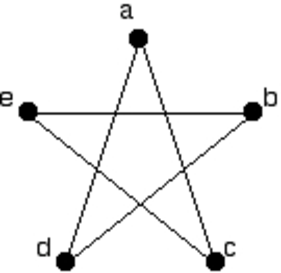
\includegraphics{star}
\end{center}

\textbf{Exercise 7}
\textsl{Show that every simple graph on $6$ vertices contains a triangle or an empty triangle.}
\begin{proof}
Let the $6$ vertices be $a$, $b$, $c$, $d$, $e$ and $f$. We see that, $a$ must have $3$ neighbors or not have $3$ neighbors since there are five other vertices. Consider the case where vertex $a$ has three neighbors. Without loss of generality let them be $b$, $c$ and $d$. If any of $b$, $c$ or $d$ are neighbors, then together with $a$ there exists a triangle. But if none of $b$, $c$ and $d$ are neighbors then those three make an empty triangle. Similarly, if $a$ is not neighbors with $b$, $c$ and $d$, then if any of $b$, $c$ and $d$ aren't neighbors we have an empty triangle. But if $b$, $c$ and $d$ are all neighbors then they form a triangle. In all cases there exists a triangle or an empty triangle.
\end{proof}

\textbf{Exercise 8}
\textsl{Show that in every simple graph the number of vertices of odd degree is even.}
\begin{proof}
Let $(V,E)$ be a graph and let $a$ be the number of vertices with even degree and $b$ be the number of vertices of odd degree. Also let $x$ be the sum of the degrees of vertices with even degree and $y$ be the sum of degrees of vertices with odd degree. Note that $x+y$ should be twice the number of edges in $(V,E)$ since $E$ is a symmetric relation and we don't allow loops. Thus $x+y=2k$ with $k \in \mathbb{Z}$. Note that regardless of the parity of $a$, $x$ must be even since it is the sum of even degrees. Thus $x = 2l$ for $l \in \mathbb{Z}$ and so $y = 2k-2l = 2(k-l)$ and since $k-l \in \mathbb{Z}$ we have $y$ is even. But then since $y$ is the sum of odd degrees, $b$ must be even, otherwise $y$ would be the odd sum of odd degrees and be odd.
\end{proof}

\textbf{Exercise 9}
\textsl{What does a graph such that every vertex has degree $2$ look like?}
\begin{proof}
Let $(V,E)$ be a finite graph with $n$ vertices such that each vertex has degree $2$. Note that the smallest $n$ can be is $3$, so let there be $3$ vertices, $a$, $b$ and $c$. We have $a$ has degree $2$ so $(a,b), (a,c) \in E$ and $b$ has degree $2$ so $(b,c) \in E$. Note that the edges for $c$ are accounted for and so $(V,E)$ must be a triangle for $n=3$. Use induction on $n$ and suppose that for a graph $(V,E)$ with $n$ vertices such that each vertex has degree $2$, one connected component is a polygon. Now let $|V| = n+1$. Consider one vertex, $a$, and consider the graph without $a$ or the two edges attached to it and instead, an edge connecting the two neighbors of $a$. Then this graph has $n$ vertices each with degree $2$, so each connected component is a polygon. But then in the original graph there was a connected component containing $a$ which was a polygon.\newline

Now suppose that $(V,E)$ is an infinite graph such that each vertex has degree $2$. Take some vertex and label it $a_0$. Arbitrarily label it's neighbors $a_1$ and $a_{-1}$. Then the other neighbors of $a_1$ and $a_{-1}$ are $a_2$ and $a_{-2}$ respectively. Continue in this way so that each vertex is labeled according to one of its neighbors and the whether the index of that vertex is positive or negative. There are two possibilities. First suppose that we reach a vertex that is already labeled. Then there are finitely many points making a cycle which means we have a connected component which is a polygon. The second case is that a vertex never gets labeled. Then this vertex isn't connected to the vertices getting labeled. Thus, the connected components of $(V,E)$ are either finite polygons or infinite lines of vertices.
\end{proof}

\textbf{Definition 10}
\textsl{Let $(V,E)$ be a graph. A walk of length $n$ from $x \in V$ to $y \in V$ is a sequence of vertices $a_0, a_1, \dots ,a_n$ where $a_0 = x$, $a_n = y$ and $(a_i, a_{i+1}) \in E$ $(0 \leq i \leq n-1)$. A path is a walk such that $a_i \neq a_j$ $(0 \leq i < j \leq n)$. A cycle is a walk such that $a_0 = a_n$ and $a_i \neq a_j$ $(0 \leq i < j \leq n)$.}\newline

\textbf{Theorem 11}
\textsl{If there is a walk from $a$ to $b$ there is a path from $a$ to $b$.}
\begin{proof}
Let $W = \{a_0, a_1, \dots , a_n\}$ such that $a_0 = a$ and $a_n = b$ be the shortest walk from $a$ to $b$. Suppose that $a_i = a_j$ for some $0 \leq i < j \leq n$. Then $W' = \{a_0, a_1, \dots , a_i, a_{j+1}, \dots , a_n\}$ is also a walk from $a$ to $b$ which is shorter than $W$. This is a contradiction and so for all $a_i, a_j \in W$ we have $a_i \neq a_j$. Thus $W$ is a path from $a$ to $b$.
\end{proof}

\textbf{Theorem 12}
\textsl{Let $\sim$ be a relation on $V$ where $a \sim b$ if there is a walk from $a$ to $b$. Then $\sim$ is an equivalence relation.}
\begin{proof}
Let $(V,E)$ be a graph and let $a,b,c \in V$. We have $a \sim a$ because of the walk of length $0$. Now let $a \sim b$. Then there exists a walk $W = \{a_0, a_1, \dots , a_n\}$ such that $a=a_0$ and $b=a_n$. Since $W$ is a walk, $(a_i, a_{i+1}) \in E$ for all $1 \leq i \leq n-1$. But then since $E$ is a symmetric relation we have $(a_{i+1}, a_i) \in E$ for all $1 \leq i \leq n-1$. Thus there exists a walk $W' = \{a_n, a_{n-1}, \dots , a_1\}$ from $b$ to $a$ and $b \sim a$. Finally suppose that $a \sim b$ and $b \sim c$. There there exists walks $W_1 = \{a_0, a_1, \dots , a_n\}$ and $W_2 = \{b_0, b_1, \dots , b_m\}$ with $a = a_0$, $b = a_n = b_0$ and $c = b_m$. Then consider $W_3 = \{c_i \mid \text{$c_i = a_i$ for $0 \leq i \leq n$ and $c_i = b_{i-n}$ for $n+1 \leq i \leq n+m$}\}$. Then $c_0 = a$ and $c_{n+m} = c$. Also $(c_i, c_{i+1}) = (a_i, a_{i+1}) \in E$ for $0 \leq i \leq n-1$ and $(c_i, c_{i+1}) = (b_i, b_{i+1}) \in E$ for $n+1 \leq i \leq n+m-1$. Additionally $(c_n, c_n+1) = (a_n, b_1) = (b_0, b_1) \in E$ which means that $W_3$ is a walk. Thus $a \sim c$ which means we've shown reflexivity, symmetry and transitivity. Therefore $\sim$ is an equivalence relation.
\end{proof}

\textbf{Definition 13}
\textsl{The connected components of a graph are its $\sim$ equivalence classes.}\newline

\textbf{Exercise 14}
\textsl{Try to define the connected components of a topological space.}\newline

Let $(X, \mathcal{A})$ be a topological space and also consider $([0;1],d_2)$. For $a,b \in X$ we say that there exists a path from $a$ to $b$ if there exists some continuous function $f \; : \; [0;1] \rightarrow X$ where $f(0) = a$ and $f(1) = b$. Then we can define a similar equivalence relation on $X$ where $a \sim b$ if there exists path from $a$ to $b$. Then the connected components will be the equivalence classes of this relation.

\textbf{Definition 15}
\textsl{A graph is connected if it only has one connected component.}\newline

\textbf{Theorem 16}
\textsl{Let $(V,E)$ be a connected graph. For $a,b \in V$ let $d(a,b)$ be the length of the shortest path from $a$ to $b$. Then $d$ is a metric on $V$.}
\begin{proof}
Let $a,b,c \in V$. A path is defined by a natural number of vertices in $V$ so it always has a length of a natural number or $0$. Thus $d(a,b) \geq 0$. Suppose that $d(a,b) = 0$. Then the shortest path is the path of length $0$ which means that $a=b$. Conversely suppose that $a=b$ then the shortest path from $a$ to $b$ is the $0$ path and so $d(a,b) = 0$.\newline

Now consider the shortest path from $a$ to $b$, $P = \{a_0, a_1, \dots , a_n\}$ where $a = a_0$ and $b = a_n$. Then since $(a_i, a_{i+1}) \in E$ for all $0 \leq i \leq n-1$ and $E$ is a symmetric relation on $V$ we have $(a_{i+1}, a_i) \in E$ as well for all $0 \leq i \leq n-1$. Then there exists a path $P' = \{a_n, a_{n-1}, \dots , a_0\}$ from $b$ to $a$. Note that this must be the shortest path because if there were a shorter one we could reverse it in the same fashion to find a shorter path from $a$ to $b$ than $P$. Thus $d(a,b) = d(b,a)$.\newline

Finally consider the shortest paths from $a$ to $b$ and $b$ to $c$, $P_1 = \{a_0, a_1, \dots , a_n\}$ and $P_2 = \{b_0, b_1, \dots , b_m\}$ where $a = a_0$, $b = a_n = b_0$ and $c = b_m$. Then consider $P_3 = \{c_i \mid \text{$c_i = a_i$ for $0 \leq i \leq n$ and $c_i = b_{i-n}$ for $n+1 \leq i \leq n+m$}\}$. Then $c_0 = a$ and $c_{n+m} = c$. Also $(c_i, c_{i+1}) = (a_i, a_{i+1}) \in E$ for $0 \leq i \leq n-1$ and $(c_i, c_{i+1}) = (b_i, b_{i+1}) \in E$ for $n+1 \leq i \leq n+m-1$. Additionally $(c_n, c_{n+1}) = (a_n, b_1) = (b_0, b_1) \in E$. Thus $P_3$ is a walk from $a$ to $c$. From Theorem 11 we know that there exists a path from $a$ to $c$ of length at most $n+m$ (23.11). Thus $d(a,c) \leq n+m = d(a,b) + d(b,c)$. Therefore $d$ is a metric.
\end{proof}

\textbf{Definition 17}
\textsl{A tree is a connected graph without cycles.}\newline

\textbf{Theorem 18}
\textsl{A graph is a tree if and only if for all vertices $a,b$ there is a unique path from $a$ to $b$.}
\begin{proof}
Let $(V,E)$ be a graph. Suppose that for all vertices $a,b \in V$ there exists a unique path from $a$ to $b$. Then $(V,E)$ is connected because $a \sim b$ for all $a,b \in V$. Let $a,b \in V$ and suppose there exists a cycle $C = \{a_0, a_1, \dots , a_n\}$ which connects $a$ and $b$. Then $a = a_i$ and $b=a_j$ for some $0 \leq i < j \leq n$. But then consider the two paths $P_1 = \{a_i, a_{i+1}, \dots , a_j\}$ and $P_2 = \{a_{j+1}, a_{j+2}, \dots , a_{n-1}, a_0, a_1, \dots , a_j\}$. Both of these are paths because $(a_i, a_{i+1}) \in E$ for all $0 \leq i \leq n-1$ and $(a_{n-1},a_0) = (a_{n-1},a_n) \in E$ and $a_i \neq a_j$ for all $0 \leq i < j \leq n$. But then there isn't a unique path from $a$ to $b$. Thus there are no cycles in $(V,E)$ and since $(V,E)$ is connected it is a tree.\newline

Conversely assume that $(V,E)$ is a tree. Then $(V,E)$ is connected and so for all $a,b \in V$ there exists a walk and therefore a path from $a$ to $b$ (23.11). Suppose that this path is not unique so that there are two paths $P_1 = \{a_0, a_1, \dots , a_n\}$ and $P_2 = \{b_0, b_1, \dots , b_m\}$ such that $a = a_0 = b_0$, $b = a_n = b_m$, $(a_i, a_{i+1}) \in E$ for all $0 \leq i \leq n-1$, $(b_i, b_{i+1}) \in E$ for all $0 \leq i \leq m-1$, $a_i \neq a_j$ for $0 \leq i < j \leq n$ and $b_i \neq b_j$ for $0 \leq i < j \leq m$. Then consider the walk $C = \{c_i \mid \text{$c_i = a_i$ for $0 \leq i \leq n$ and $c_i = b_{n+m-i}$ for $n+1 \leq i \leq n+m-1$}\}$. Note that $C$ is a walk because $(c_i, c_{i+1}) = (a_i, a_{i+1}) \in E$ for all $0 \leq i \leq n-1$ and $(c_i, c_{i+1}) = (b_{n+m-i}, b_{n+m-(i+1)}) \in E$ for all $n+1 \leq i \leq n+m-1$ and $(c_n, c_{n+1}) = (a_n, b_{m-1}) = (b_m, b_{m-1}) \in E$. But also $c_i = a_i \neq a_j = c_j$ for all $0 \leq i < j \leq n-1$ and $c_i = b_{n+m-i} \neq b_{n+m-j} = c_j$ for $n+1 \leq i < j \leq n+m-1$ and $c_n = a_n \neq a_i$ for $0 \leq i < n$ and $c_n = b_m \neq b_i$ for $0 \leq i < m$. Therefore, since $c_0 = a_0 = b_0 = c_{m+n}$, $C$ is a cycle, which doesn't exist in a tree. Thus there must be a unique path from $a$ to $b$.
\end{proof}

\textbf{Theorem 19}
\textsl{Let a leaf be a vertex of degree $1$. Then every finite tree on $n \geq 2$ vertices has a leaf.}
\begin{proof}
Let $(V,E)$ be a tree on $n \geq 2$ vertices. Consider the longest path on $(V,E)$, $P = \{a_0, a_1, \dots , a_m\}$. If $a_0$ or $a_m$ had degree greater than $1$ then there would exist a longer path than $P$. Thus $a_0$ and $a_m$ have degree $1$ and are leaves.
\end{proof}

\textbf{Theorem 20}
\textsl{A tree on $n$ vertices has $n-1$ edges.}
\begin{proof}
Note that a tree with one vertex has $1-1 = 0$ edges. Induct on $n$ and assume that a tree on $n$ vertices has $n-1$ edges. Consider a tree on $n+1$ vertices. This tree has a leaf, $a$, and so consider the same graph without $a$ and its corresponding edge. Since $a$ has only one edge, removing it maintained all paths on the graph and created no new cycles. Thus the new graph is still a connected graph with no cycles and is therefore a tree on $n$ vertices. Thus it has $n-1$ edges. But then the original graph on $n+1$ vertices must have $n$ edges as desired.
\end{proof}

\textbf{Theorem 21}
\textsl{Every finite tree on $n \geq 2$ vertices has at least $2$ leaves.}
\begin{proof}
Let $(V,E)$ be a tree on $n \geq 2$ vertices. Consider the longest path on $(V,E)$, $P = \{a_0, a_1, \dots , a_m\}$. If $a_0$ or $a_m$ had degree greater than $1$ then there would exist a longer path than $P$. Thus $a_0$ and $a_m$ have degree $1$ and are leaves.
\end{proof}

\textbf{Theorem 22}
\textsl{The only tree on $n \geq 2$ vertices with exactly two leaves is a path.}
\begin{proof}
Let $(V,E)$ be a tree on $n \geq 2$ vertices with exactly two leaves, $a$ and $b$. Note that for $n = 2$ we have $(a,b) \in E$ so there exists a path from $a$ to $b$ which means $(V,E)$ is a path. Use induction on $n$ and assume that for $n \geq 2$, $(V,E)$ is a path. Now let $(V,E)$ have $n+1$ vertices and exactly two leaves, $a$ and $b$. Let $(a,a') \in E$. Consider the graph after removing $a$ and $(a,a')$. By removing a vertex of degree $1$ all paths are maintained and no cycles are created. Thus, the new graph is still a tree. Then it has at least two leaves, one of which is $b$ (23.21). Note that if there exists another leaf, then it would be in $(V,E)$ where $|V| = n+1$. Therefore the graph with $n$ vertices has exactly two leaves and is therefore a path. But then $(V,E)$ with $n+1$ vertices must be a path as well since only one edge was taken away.
\end{proof}

\textbf{Definition 23}
\textsl{Let $(V,E)$ be a graph. A walk $a_0, a_1, \dots , a_n$ is Eulerian if $a_0 = a_n$ and it uses every edge exactly once (that is, for all $e \in E$ there is a unique $0 \leq i < n$ such that $(a_i,a_{i+1}) = e$ as an undirected pair.}\newline

\textbf{Theorem 24}
\textsl{A simple graph has an Eulerian walk on it if and only if it is connected and every vertex has even degree.}
\begin{proof}
Let $(V,E)$ be a simple graph and suppose that there exists an Eulerian walk on it. Then there exists a walk $W = \{a_0, a_1, \dots , a_n\}$ such that $a_0 = a_n$ and for all $e \in E$ there exists a unique $0 \leq i < n$ such that $(a_i, a_{i+1}) = e$. But since $a_0 = a_n$, each vertex in $V$ must have an even degree so that for all $(a_i, a_{i+1}) \in E$ there exists $(a_{i+1}, a_{i+2})$ for $0 \leq i < n-1$. That is, each vertex reached on the path by some edge must have a different edge leaving it, which means the degree is even.\newline

Conversely, assume that $(V,E)$ is connected, has $n$ vertices and each has even degree. Note that if $n=1$ then we're done, so assume that $n \geq 2$. Consider some vertex $a_0 \in V$. Let $W = \{a_0, a_1, \dots , a_m\}$ be the longest walk such that $a_0 = a_m$ and for all $0 \leq i < j \leq m-1$ we have $(a_i, a_{i+1}) \neq (a_j, a_{j+1})$. That is, every edge is traversed only once. Note that this walk exists because $(V,E)$ is connected, so there is a walk between any two vertices, $(V,E)$ is finite so there are finitely many vertices and each vertex has even degree so for $a_i \in W$ with $0 < i < m$ there exists both $(a_{i-1}, a_i)$ and $(a_i, a_{i+1})$. Now suppose that this walk is no Eulerian. Then there exists some edge $e \in E$ such that for all $0 \leq i < m$, $(a_i, a_{i+1}) \neq e$. Note that if every edge with the properties of $e$ is not connected to some $a_i$ then $(V,E)$ is not connected. Thus we can assume $e$ connects two vertices in $(V,E)$, one of which is some $a_i \in W$ and we call the other $b_1$. Consider a new walk, $W' = \{b_0, b_1, \dots, b_k\}$ such that $a_i = b_0 = b_k$ and each edge is only traversed once, as in $W$. Note that we can make this walk such that $(b_i, b_{i+1}) \neq (a_j, a_{j+1})$ for all $0 \leq i < k$ and $0 \leq i < m$ because $b_1 \neq a_i$ for all $0 \leq i < m$ and some edge in $W'$ was also in $W$ then some $a_i$ would have odd degree. Thus $W'$ traverses each edge only once and uses no edges from $W$. Consider a new walk $W'' = \{a_0, a_1, \dots , a_i, \dots b_1, b_2, \dots , b_{k-1}, a_{i+1}, \dots , a_m\}$. This walk traverses each edge only once and $a_0 = a_m$, but it is longer than $W$, which is a contradiction. Thus $W$ must be an Eulerian walk on $(V,E)$.
\end{proof}

\end{flushleft}

\newpage

\begin{flushright}
Kris Harper

MATH 16300

Mikl\'{o}s Ab\'{e}rt

May 27, 2008
\end{flushright}

\begin{flushleft}

\Large

Sheet 25: Complex Numbers\newline

\normalsize

\textbf{Definition 1}
\textsl{A complex number is a an ordered pair of real numbers. The set of complex numbers is denoted by $\mathbb{C}$.}\newline

\textbf{Definition 2}
\textsl{For $z_1 = (a_1,b_1) \in \mathbb{C}$ and $z_2 = (a_2,b_2) \in \mathbb{C}$ let
\[
z_1 + z_2 = (a_1 + a_2, b_1 + b_2)
\]
and let
\[
z_1 \cdot z_2 = (a_1a_2 - b_1b_2, a_1b_2 + a_2b_1).
\]}\newline

\textbf{Theorem 3}
\textsl{$\mathbb{C}$ endowed with $+$ and $\cdot$ is a commutative ring.}
\begin{proof}
Let $z_1 = (a_1,b_1) \in \mathbb{C}$, $z_2 = (a_2,b_2) \in \mathbb{C}$ and $z_3 = (a_3,b_3) \in \mathbb{C}$. Then note that
\[
z_1 + z_2 = (a_1 + a_2, b_1 + b_2) = (a_2 + a_1, b_2 + b_1) = z_2 + z_1.
\]
Also
\begin{align*}
(z_1 + z_2) + z_3 &= (a_1 + a_2, b_1 + b_2) + (a_3, b_3) \\
			    &= (a_1 + a_2 + a_3, b_1 + b_2 + b_3) \\
			    &= (a_1 + (a_2 + a_3), b_1 + (b_2 + b_3)) \\
			    &= (a_1, b_1) + (a_2 + a_3, b_2 + b_3) \\
			    &= z_1 + (z_2 + z_3).
\end{align*}
Furthermore let $0 = (0, 0)$ so we have
\[
z_1 + 0 = (a_1, b_1) + (0, 0) = (a_1 + 0, b_1 + 0) = (a_1, b_1) = z_1
\]
Supposing there are two distinct $0$s we have $0 = 0 + 0' = 0' + 0 = 0'$ which shows that $0$ is unique. Letting $-z_1 = (-a_1, -b_1)$ we have
\[
z_1 + -z_1 = (a_1, b_1) + (-a_1, -b_1) = (a_1 + -a_1, b_1 + -b_1) = (0, 0) = 0.
\]
Supposing there are two distinct values of $-z_1$ we have $z_1 + (-z_1) = 0$ and $z_1 + (-z_1') = 0$. Then
\begin{align*}
-z_1 &= -z_1 + 0 \\
	&= -z_1 + (0, 0) \\
	&= -z_1 + (a_1 - a_1, b_1 - b_1) \\
	&= -z_1 + (a_1, b_1) + (-a_1, -b_1) \\
	&= -z_1 + z_1 + (-a_1, -b_1) \\
	&= -z_1' + z_1 + (-a_1, -b_1) \\
	&= -z_1' + (a_1, b_1) + (-a_1, -b_1) \\
	&= -z_1' + (a_1 - a_1, b_1 - b_1) \\
	&= -z_1' + (0,0) \\
	&= -z_1' + 0 \\
	&= -z_1'
\end{align*}
So we have shown additive commutativity, associativity, identity and inverse. Now consider
\[
z_1 \cdot z_2 = (a_1a_2 - b_1b_2, a_1b_2 + a_2b_1) = (a_2a_1 - b_2b_1, a_2b_1 + a_1b_2) = z_2 \cdot z_1.
\]
Also
\begin{align*}
(z_1 \cdot z_2) \cdot z_3 &= (a_1a_2 - b_1b_2, a_1b_2 + a_2b_1) \cdot (a_3, b_3) \\
	&= (a_3(a_1a_2 - b_1b_2) - b_3(a_1b_2 + a_2b_1), b_3(a_1a_2 - b_1b_2) + a_3(a_1b_2 + a_2b_1)) \\
	&= (a_1a_2a_3 - a_3b_1b_2 - a_1b_2b_3 - a_2b_1b_3, a_1a_2b_3 - b_1b_2b_3 + a_1a_3b_2 + a_2a_3b_1) \\
	&= (a_1(a_2a_3 - b_2b_3) - b_1(a_2b_1 + a_3b_2), b_1(a_2a_3 - b_2b_3) + a_1(a_2b_3 + a_3b_2)) \\
	&= (a_1, b_1) \cdot (a_2a_3 - b_2b_3, a_2b_3 + a_3b_2) \\
	&= z_1 \cdot (z_2 \cdot z_3)
\end{align*}
Let $1 = (1,0)$ so we have
\[
z_1 \cdot 1 = (a_1, b_1) \cdot (1, 0) = (a_1 \cdot 1 - b_1 \cdot 0, a_1 \cdot 0 + b_1 \cdot 1) = (a_1, b_1) = z_1.
\]
Supposing there are two distinct $1$s we have $1 = 1 \cdot 1' = 1' \cdot 1 = 1'$ which shows that $1$ is unique. Finally note that
\begin{align*}
z_1 \cdot (z_2 + z_3) &= (a_1, b_1) \cdot ((a_2, b_2) + (a_3, b_3)) \\
	&= (a_1, b_1) \cdot (a_2 + a_3, b_2 + b_3) \\
	&= (a_1(a_2 + a_3) - b_1(b_2 + b_3), a_1(b_2 + b_3) + b_1(a_2 + a_3)) \\
	&= (a_1a_2 + a_1a_3 - b_1b_2 - b_1b_3, a_1b_2 + a_1b_3 + b_1a_2 + b_1a_3) \\
	&= (a_1a_2 - b_1b_2 + a_1a_3 - b_1b_3, a_1b_2 + a_2b_1 + a_1b_3 + a_3b_1) \\
	&= (a_1a_2 - b_1b_2, a_1b_2 + a_2b_1) + (a_1a_3 - b_1b_3, a_1b_3 + a_3b_1) \\
	&= (a_1, b_1) \cdot (a_2, b_2) + (a_1, b_1) \cdot (a_3, b_3) \\
	&= z_1 \cdot z_2 + z_1 \cdot z_3.
\end{align*}
Thus we have shown multiplicative commutativity, associativity and identity as well as distributivity. Therefore $\mathbb{C}$ is a commutative ring.
\end{proof}

\textbf{Definition 4}
\textsl{The imaginary number
\[
i = (0,1).
\]}\newline

\textbf{Theorem 5}
\textsl{Define $\varphi \; : \; \mathbb{R} \rightarrow \mathbb{C}$ be defined by $\phi (x) = (x,0)$. Then $\varphi$ is injective and for all $x,y \in \mathbb{R}$ we have $\varphi (x+y) = \varphi (x) + \varphi (y)$ and $\varphi (xy) = \varphi(x) \cdot \varphi (y)$.}
\begin{proof}
Let $x_1, x_2 \in \mathbb{R}$ such that $x_1 \neq x_2$. Then $\varphi (x_1) = (x_1, 0)$ and $\varphi (x_2) = (x_2, 0)$. But since $x_1 \neq x_2$ we have $(x_1, 0) \neq (x_2, 0)$ and so $\varphi$ is injective. Now let $x,y \in \mathbb{R}$. Then we have
\[
\varphi (x+y) = (x+y,0) = (x+y,0+0) = (x,0) + (y,0) = \varphi (x) + \varphi (y).
\]
Also
\[
\varphi (xy) = (xy,0) = (xy - 0 \cdot 0, x \cdot 0 + y \cdot 0) = (x,0) \cdot (y,0) = \varphi (x) \cdot \varphi (y).
\]
\end{proof}

\textbf{Lemma 6}
\textsl{We have
\[
i \cdot i = -1
\]}
\begin{proof}
We have
\[
i \cdot i = (0,1) \cdot (0,1) = (0\cdot 0 - 1 \cdot 1, 0 \cdot 1 + 0 \cdot 1) = (-1,0) = \varphi (-1) = 1.
\]
\end{proof}

\textbf{Definition 7}
\textsl{Let $z = (a,b)$ be a complex number. Then the real part
\[
\text{Re} \, z = a
\]
and the imaginary part
\[
\text{Im} \, z = b.
\]}\newline

\textbf{Lemma 8}
\textsl{Let $z$ be a complex number. Then we have
\[
z = \text{Re} \, z + i \cdot \text{Im} \, z.
\]}
\begin{proof}
Let $z = (a,b)$. We have
\begin{align*}
z &= (a,b) \\
  &= (a+0,0+b) \\
  & = (a,0) + (0,b) \\
  &= \varphi (a) + (0 \cdot b - 1 \cdot 0, 0 \cdot 0 + b \cdot 1) \\
  &= a + (0,1) \cdot (b,0) \\
  &= a + i \cdot \varphi (b) \\
  & = a + i \cdot b \\
  & = \text{Re} \, z + i \cdot \text{Im} \, z.
\end{align*}
\end{proof}

\textbf{Definition 9}
\textsl{Let $z = a + bi$ be a complex number. Then the complex conjugate of $z$ is
\[
\overline{z} = a - bi.
\]}\newline

\textbf{Lemma 10}
\textsl{For $0 \neq z \in \mathbb{C}$ we have
\[
z \frac{\overline{z}}{z \overline{z}} = 1.
\]
That is,
\[
z^{-1} = \frac{\overline{z}}{z \overline{z}}.
\]}
\begin{proof}
Let $z = a+bi$. We have
\[
\frac{z \overline{z}}{z \overline{z}} = \frac{(a+bi)(a-bi)}{(a+bi)(a-bi)} = \frac{a^2+b^2}{a^2+b^2} = 1.
\]
\end{proof}

\textbf{Exercise 11}
\textsl{Show that $(1+i)/(2+3i) = (5-i)/13$.}
\begin{proof}
We have
\[
\frac{1+i}{2+3i} = \frac{(1+i)(2-3i)}{(2+3i)(2-3i)} = \frac{2-i+3}{13} = \frac{5-i}{13}.
\]
\end{proof}

\textbf{Definition 12}
\textsl{For $z \in \mathbb{C}$ let the absolute value of $z$ be
\[
|z| = \sqrt{z \overline{z}}.
\]}\newline

\textbf{Theorem 13}
\textsl{Let $z$ and $w$ be complex numbers. Then the following hold:\newline
1) $\overline{\overline{z}} = z$;\newline
2) $\overline{z} = z$ if and only if $z$ is real;\newline
3) $\overline{z+w} = \overline{z} + \overline{w}$;\newline
4) $-\overline{z} = \overline{-z}$;\newline
5) $\overline{zw} = \overline{z} \cdot \overline{w}$;\newline
6) $\overline{z^{-1}} = \overline{z}^{-1}$ if $z \neq 0$;\newline
7) $|z| = 0$ if and only if $z = 0$;\newline
8) $|z+w| \geq |z| + |w|$;\newline
9) $|zw| = |z||w|$.}
\begin{proof}
Let $z = a+bi$ and $w = c+di$.\newline

1) $\overline{\overline{z}} = \overline{a-bi} = a - (-bi) = a+bi = z$.\newline

2) Let $\overline{z} = z$. Then $a-bi = a+bi$ which means $-b = b$ so $b = 0$. Thus $z$ has no imaginary part and is real. Now suppose $z$ is real. Then $b=0$ so we have $\overline{z} = a = z$.\newline

3) $\overline{z+w} = \overline{a+c + (b+d)i} = a+c -(b+d)i = a-bi + c-di = \overline{z} + \overline{w}$.\newline

4) $-\overline{z} = -(a-bi) = (-a + bi) = \overline{-z}$.\newline

5) $\overline{zw} = \overline{ac-bd + (ad + bc)i} = ac-bd-adi-bci = (a-bi) \cdot (c-di) = \overline{z} \cdot \overline{w}$. \newline

6) Let $z \neq 0$. Then
\[
\overline{z^{-1}} = \overline{\frac{\overline{z}}{z \overline{z}}} = \overline{\frac{a-bi}{a^2 + b^2}} = \frac{a}{a^2 + b^2} + \frac{bi}{a^2+b^2} = \frac{a+bi}{a^2 + b^2} = \frac{z}{z \overline{z}} = \overline{z}^{-1}.
\]

7) Let $|z| = 0$. Then $0 = \sqrt{z \overline{z}} = \sqrt{a^2 + b^2}$ so $a^2 + b^2 = 0$ and since $a^2$ and $b^2$ are both greater than or equal to $0$, they must both be $0$. Then $a = b = 0$ so $z = 0$. Now suppose $z = 0$. Then $|z| = \sqrt{z \overline{z}} = \sqrt{a^2 + b^2} = \sqrt{0} = 0$.\newline

8) We have
\[
b^2c^2 + a^2d^2 -2abcd = (ad-bc)^2 \geq 0
\]
so
\[
b^2c^2 + a^2d^2 \geq 2abcd
\]
and
\[
(a^2 + b^2)(c^2 + d^2) = a^2c^2 +b^2c^2 + a^2d^2 + b^2d^2 \geq a^2c^2 + 2abcd + b^2d^2 = (ac+bd)^2.
\]
Then we have
\[
2 \sqrt{(a^2 + b^2)(c^2 + d^2)} \geq 2(ac+bd)
\]
so
\begin{align*}
(|z| + |w|)^2 &= (\sqrt{a^2 + b^2} + \sqrt{c^2 + d^2})^2 \\
		   &= a^2 + b^2 + 2 \sqrt{(a^2 + b^2)(c^2 + d^2)} + c^2 + d^2 \\
		   & \geq a^2 + b^2 + 2(ac+bd) + c^2 + d^2 \\
		   &= (a+c)^2 + (b+d)^2 \\
		   &= |z+w|^2.
\end{align*}
Thus $|z| + |w| \geq |z+w|$.\newline

9) We have
\begin{align*}
|zw| &= |(ac-bd) + (ad+bc)i| \\
	&= \sqrt{(ac-bd)^2 + (ad+bc)^2} \\
	&= \sqrt{a^2c^2 -2abcd + b^2d^2 + a^2d^2 + 2abcd + b^2c^2} \\
	&= \sqrt{a^2c^2 + b^2d^2 + a^2d^2 + b^2c^2} \\
	&= \sqrt{(a^2 + b^2)(c^2 + d^2)} \\
	&= \sqrt{a^2 + b^2} \sqrt{c^2 + d^2} \\
	&= |z||w|.
\end{align*}
\end{proof}

\textbf{Definition 14}
\textsl{Let $z \in \mathbb{C}$. A real number $\alpha$ satisfying the equality $z = |z| (\cos \alpha + i \sin \alpha)$ is called an argument of $z$.}\newline

\textbf{Theorem 15}
\textsl{If $\alpha$ and $\beta$ are arguments of $z$ then $\alpha - \beta = 2k \pi$ for some $k \in \mathbb{Z}$.}
\begin{proof}
Let $\alpha$ and $\beta$ be arguments of $z$. Then $z = |z| (\cos \alpha + i \sin \alpha) = |z| (\cos \beta + i \sin \beta)$ so $\cos \alpha + i\sin \alpha = \cos \beta + i\sin \beta$. Multiplying both sides by $\cos \beta - i \sin \beta$ we have
\begin{align*}
\cos (\alpha - \beta) + i \sin (\alpha - \beta) &= \cos \alpha \cos \beta + \sin \alpha \sin \beta + i (\sin \alpha \cos \beta - \sin \beta \cos \alpha) \\
	&= \cos \alpha \cos \beta + i \sin \alpha \cos \beta - i \sin \beta \cos \alpha + \sin \alpha \sin \beta \\
	&= (\cos \alpha + i \sin \alpha)(\cos \beta - i \sin \beta) \\
	&= (\cos \beta + i \sin \beta)(\cos \beta - i \sin \beta) \\
	&= \cos^2 \beta + \sin^2 \beta \\
	&= 1.
\end{align*}
Thus $(\cos (\alpha - \beta) + i \sin (\alpha - \beta)) = 1$ which only occurs if $\cos (\alpha - \beta) = 1$ and $i \sin (\alpha - \beta) = 0$. Thus $\alpha - \beta = 2k \pi$ for $k \in \mathbb{Z}$.
\end{proof}

\textbf{Theorem 16}
\textsl{Let $z = |z| (\cos \alpha + i \sin \alpha)$ and $w = |w| (\cos \beta + i \sin \beta)$. Then
\[
zw = |z||w| (\cos (\alpha + \beta) + i \sin (\alpha + \beta))
\]}
\begin{proof}
We have
\begin{align*}
zw &= (|z| (\cos \alpha + i \sin \alpha)) (|w| (\cos \beta + i \sin \beta)) \\
    &= |z||w| (\cos \alpha \cos \beta - \sin \alpha \sin \beta + i (\sin \alpha \cos \beta + \cos \alpha \sin \beta)) \\
    &= |z||w| (\cos (\alpha+\beta) + i \sin (\alpha + \beta)).
\end{align*}
\end{proof}

\textbf{Corollary 17}
\textsl{Let $z = |z| (\cos \alpha + i \sin \alpha)$. Then
\[
z^n = |z|^n (\cos n \alpha + i \sin n \alpha).
\]}
\begin{proof}
Note that for $n=1$ we have $z^1 = z = |z| (\cos \alpha + i \sin \alpha) = |z|^1 (\cos (1 \cdot \alpha) + i \sin (1 \cdot \alpha))$. Induct on $n$ and assume that for $n \in \mathbb{N}$ we have $z^n = |z|^n (\cos n \alpha + i \sin n \alpha)$. Then from Theorem 16 we have
\begin{align*}
z^{n+1} &= z \cdot z^n \\
	   &= (|z| (\cos \alpha + i \sin \alpha)) (|z|^n (\cos n \alpha + i \sin n \alpha)) \\
	   &= |z|^{n+1} (\cos (n+1) \alpha + i \sin (n+1) \alpha)
\end{align*}
as desired (25.17).
\end{proof}

\textbf{Definition 18}
\textsl{A complex number $z$ is an $n$th root of unity if it satisfies
\[
z^n = 1.
\]}\newline

\textbf{Theorem 19}
\textsl{Let $n$ be a natural number. Then there are exactly $n$ $n$th roots of unity, namely
\[
\varepsilon_{n,k} = \cos \left ( k \frac{2 \pi}{n} \right ) + i \sin \left ( k \frac{2 \pi}{n} \right ) \textup{ for } 0 \leq k \leq n-1.
\]}
\begin{proof}
Note that from Theorem 21 we know that there are at most $n$ roots of the polynomial $x^n - 1$ which means there are at most $n$ solutions to the equation $x^n = 1$. From Corollary 17 we know
\[
\varepsilon_{n,k}^n = \cos \left ( k 2 \pi \right ) + i \sin \left ( k 2 \pi \right ) = 1
\]
where $0 \leq k \leq n-1$ (25.17). Suppose that there are two values of $k$, $k_1 \neq k_2$, such that $\varepsilon_{n,k_1} = \varepsilon_{n,k_2}$. Then we have
\[
\cos \left ( k_1 \frac{2 \pi}{n} \right ) + i \sin \left ( k_1 \frac{2 \pi}{n} \right ) = \cos \left ( k_2 \frac{2 \pi}{n} \right ) + i \sin \left ( k_2 \frac{2 \pi}{n} \right ).
\]
But then $(2 k_1 \pi)/n - (2 k_2 \pi)/n = 2 m \pi$ for some $m \in \mathbb{Z}$ (25.15). Thus $k_1 - k_2 = mn$ and $k_2 - k_1 = -mn$. Note that $m \neq 0$ because $k_1 \neq k_2$ and so the positive difference between $k_1$ and $k_2$ must be greater than or equal to $n$. But we have $0 \leq k_1, k_2 \leq n-1$, so $k_i - k_j < n$ for all values of $k$. Thus for distinct values of $k$ we have distinct values of $\varepsilon_{n,k}$. Therefore there are least and at most $n$ $n$th roots of unity which means there are $n$ $n$th roots of unity.
\end{proof}

\textbf{Theorem 20}
\textsl{Let $0 \neq z \in \mathbb{C}$ and let $n \in \mathbb{N}$. Then there are exactly $n$ complex numbers satisfying the equality
\[
w^n = z.
\]}
\begin{proof}
Let $z = |z| \left ( \cos \left (\alpha \right ) + i \sin \left ( \alpha \right ) \right )$. Then from Theorem 21 we know that there are at most $n$ values satisfying $w^n = z$. Consider
\[
w = |z|^{1/n} \left ( \cos \left ( \frac{\alpha + 2 k \pi}{n} \right ) + i \sin \left ( \frac{\alpha + 2 k \pi}{n} \right ) \right ).
\]
Then
\begin{align*}
w^n &= |z| \left ( \cos \left ( \alpha + 2k \pi \right ) + i \sin \left ( \alpha + 2k \pi \right ) \right )\\
	&= |z| \left ( \cos \left ( \alpha \right ) + i \sin \left ( \alpha \right ) \right ) \\
	&= z.
\end{align*}
from Corollary 17 (25.17). We know that each of the values $0 \leq k \leq n-1$ is distinct using a similar argument as in Theorem 19.
\end{proof}

\textbf{Theorem 21}
\textsl{Let $p(x) \in \mathbb{C}[x]$ be a complex polynomial of degree $n$. Then $p(x)$ has at most $n$ roots.}
\begin{proof}
Suppose that $\deg(p) = n$ and $p$ has $m$ distinct roots with $m>n$. Let the $m$ roots be $\alpha_1, \alpha_2, \dots ,\alpha_m$. In the case where $\alpha_i = \alpha_j$ for all $1 \leq i,j < m$ we have $p(x) = (x-\alpha_1)^m$ which has degree higher than $n$. Thus we can assume that there exists two $\alpha_i$ and $\alpha_j$ such that $\alpha_i \neq \alpha_j$ and $i \neq j$. We know that $p = (x-\alpha_i)q_i$ for some $q \in \mathbb{C}[x]$ (19.8). We also know that since $\alpha_j$ is a root of $p$ it is a root of $(x-\alpha_i)$ or $q_i$ (19.7). Since $\alpha_j-\alpha_i \neq 0$, $\alpha_j$ is a root of $q_i$. Thus $q_i = (x-\alpha_j)q_j$ and $p = (x-\alpha_i)(x-\alpha_j)q_j$ (19.8). We can continue in this process $m$ times until we have
\[
p = \prod_{i=1}^m (x-\alpha_i) q_m.
\]
But then $\deg(p) = m \neq n$ which is a contradiction.
\end{proof}

\textbf{Exercise 22}
\textsl{Where is the mistake in the following?
\[
1 = \sqrt{1} = \sqrt{-1 \cdot -1}  = \sqrt{-1} \cdot \sqrt{-1} = i \cdot i = -1.
\]}

The square root function is only defined for non-negative real numbers. It makes no sense to say $\sqrt{-1 \cdot -1} = \sqrt{-1} \cdot \sqrt{-1}$ because $\sqrt{-1}$ is meaningless.\newline

\textbf{Exercise 23}
\textsl{Let $u,w$ be complex numbers. Find the complex numbers $z$ such that $u,w,z$ form a equilateral triangle. Express the centers of these triangles.}
\begin{proof}
Given the three points $u,w,z$, the centroid of the triangle formed by them should be
\[
x = \frac{u+w+z}{3}.
\]
Given this and the two points $u$ and $w$ we want the condition each of $u$ $w$ and $z$ are a distance $L$ from the center, $x$, and are separated by an angle of $2 \pi /3$. Thus
\[
u-x = L \left ( \cos \left ( \alpha \right ) + i \sin \left ( \alpha \right ) \right ),
\]
\[
z-x = L \left ( \cos \left ( \alpha - \frac{2 \pi}{3} \right ) + i \sin \left ( \alpha - \frac{2 \pi}{3} \right ) \right )
\]
and
\[
w-x = L \left ( \cos \left ( \alpha + \frac{2 \pi}{3} \right ) + i \sin \left ( \alpha + \frac{2 \pi}{3} \right ) \right )
\]
for some angle $\alpha$. This implies that $(u-x)(w-x) = (z-x)^2$ which after substituting for $x$ and expanding gives us
\[
u^2 + w^2 + z^2 = uw + uz + wz.
\]
Using the quadratic formula to solve for $z$ we end up with
\[
z = \frac{u + w \pm i \sqrt{3}(u-w)}{2}.
\]
The center of the triangle is then at
\[
\frac{u+w}{2} \pm \frac{i \sqrt{3} (u-w)}{6}.
\]
\end{proof}

\textbf{Exercise 24}
\textsl{Take an arbitrary and draw an equilateral triangle on all sides looking outward. Prove that the centers of these triangles forms an equilateral triangle.}
\begin{proof}
Let $a$, $b$ and $c$ be vertices of an equilateral triangle and $x$, $y$ and $z$ be the centers of the outer equilateral triangles formed. Then
\[
x = \frac{a+b}{2} \pm \frac{i \sqrt{3} (a-b)}{6},
\]
\[
y = \frac{b+c}{2} \pm \frac{i \sqrt{3} (b-c)}{6}
\]
and
\[
z = \frac{c+a}{2} \pm \frac{i \sqrt{3} (c-a)}{6}.
\]
Then we can verify that
\[
x^2 + y^2 + z^2 = xy + yz + xz
\]
which is the condition we had earlier for an equilateral triangle.
\end{proof}

\textbf{Exercise 25}
\textsl{Compute $(1+i)^{2006}$.}\newline

Let $z = 1+i$. Note that $|z| = \sqrt{z \overline{z}} = \sqrt{2}$. Then let $\alpha = \pi/4$ so that
\[
z = \sqrt{2} \left ( \frac{1}{\sqrt{2}} + \frac{i}{\sqrt{2}} \right ) = |z| (\cos \alpha + i \sin \alpha).
\]
Then
\[
z^{2006} = \sqrt{2}^{2006} \left ( \cos \left ( \frac{1003 \pi}{2} \right ) + i \sin \left ( \frac{1003 \pi}{2} \right ) \right ) = -i 2^{1003}\]

\textbf{Exercise 26}
\textsl{What is the sum of the $n$th roots of unity?}
\begin{proof}
Note that the $k$th root of unity is given by
\[
\varepsilon_{n,k} = \cos \left ( k \frac{2 \pi}{n} \right ) + i \sin \left ( k \frac{2 \pi}{n} \right ).
\]
Let $n > 1$ and let $k = 1$. Then
\[
\varepsilon_{n,1} = \cos \left (\frac{2 \pi}{n} \right ) + i \sin \left (\frac{2 \pi}{n} \right ) \neq 1
\]
and the arguments of $\varepsilon_{n,k}$ are $(2 \pi)/n$. But then
\begin{align*}
\varepsilon_{n,1}^k &= |\varepsilon_{n,1}| \left ( \cos \left ( k \frac{2 \pi}{n} \right ) + i \sin \left ( k \frac{2 \pi}{n} \right ) \right ) \\
			    &= \cos \left ( k \frac{2 \pi}{n} \right ) + i \sin \left ( k \frac{2 \pi}{n} \right ) \\
			    &= \varepsilon_{n,k}
\end{align*}
by Corollary 17 (25.17). Thus if we have one nontrivial root of unity we can find the rest by taking powers of the first for powers $0 \leq k \leq n-1$. But then
\[
\sum_{k=0}^{n-1} \varepsilon_{n,k} = \sum_{k=0}^{n-1} \varepsilon_{n,1}^k = \frac{1-\varepsilon_{n,1}^n}{1-\varepsilon_{n,1}} = 0
\]
because $\varepsilon_{n,1} = 1$.
\end{proof}

\textbf{Exercise 27}
\textsl{What is the product of the $n$th roots of unity?}
\begin{proof}
Similarly
\[
\prod_{k=0}^{n-1} \varepsilon_{n,k} = \prod_{k=0}^{n-1} \varepsilon_{n,1}^k = \varepsilon_{n,1}^{\frac{n(n-1)}{2}}.
\]
For $n$ odd we can write this as
\[
\left ( \varepsilon_{n,1}^n \right )^{\frac{n-1}{2}} = 1.
\]
For $n$ even we can write
\[
\left ( \varepsilon_{n,1}^{\frac{n}{2}} \right )^{n-1}.
\]
Note that
\[
\varepsilon_{n,1}^{\frac{n}{2}} = |\varepsilon_{n,1}|^{\frac{n}{2}} \left ( \cos \left ( \frac{n}{2} \frac{2 \pi}{n} \right ) + i \sin \left ( \frac{n}{2} \frac{2 \pi}{n} \right ) \right ) = \cos \pi + i \sin \pi = -1.
\]
Thus we have $-1^{n-1}$ and since $n$ is even this is $-1$. Therefore the product of the $n$th roots of unity is $1$ for $n$ odd and $-1$ for $n$ even.
\end{proof}

\textbf{Exercise 28}
\textsl{What is the sum of the squares of the $n$th roots of unity?}
\begin{proof}
We have
\[
\sum_{k=0}^{n-1} \varepsilon_{n,k}^2 = \sum_{k=0}^{n-1} \varepsilon_{n,1}^{2k} = \varepsilon_{n,1}^0 + \varepsilon_{n,1}^2 + \dots + \varepsilon_{n,1}^{2n-2}.
\]
If we multiply both sides of this equation by $1-\varepsilon_{n,1}^2$ we have
\[
\sum_{k=0}^{n-1} \varepsilon_{n,1}^{2k} = \frac{1-\varepsilon_{n,1}^{2n}}{1-\varepsilon_{n,1}^2} = \frac{1 - \left ( \varepsilon_{n,1}^n \right )^2}{1 - \varepsilon_{n,1}} = 0.
\]
\end{proof}

\end{flushleft}

\newpage

\begin{flushright}
Kris Harper

MATH 16300

Mikl\'{o}s Ab\'{e}rt

May 27, 2008
\end{flushright}

\begin{flushleft}

\Large

Sheet 26: Log and Exp\newline

\normalsize

\textbf{Definition 1}
\textsl{For $x > 0$ let
\[
\log x = \int_1^x \frac{1}{t}dt.
\]}

\textbf{Theorem 2}
\textsl{If $x,y > 0$ then
\[
\log (xy) = \log x + \log y.
\]}
\begin{proof}
Let $f(x) = \log(xy)$. Then $f'(x) = \log' (xy) = (1/xy)y = 1/x = \log' x$ (21.16, 22.17). Then $\log (xy) = \log (x) + c$ for some constant $c$. Letting $x = 1$ we have $\log y = 0 + c$ so we must have $\log (xy) = \log x + \log y$.
\end{proof}

\textbf{Corollary 3}
\textsl{For a natural number $n$ and $x > 0$ we have
\[
\log (x^n) = n \log x.
\]}
\begin{proof}
Note that for $n=1$ we have $\log x = \log x$. Induct on $n$ and assume that for some $n \in \mathbb{N}$ we have $\log (x^n) = n \log x$. Consider
\[
\log (x^{n+1}) = \log(x \cdot x^n) = \log x + \log (x^n) = \log x + n \log x = (n+1) \log x
\]
by Theorem 2 (26.2). Then by mathematical induction the statement must be true for all $n \in \mathbb{N}$.
\end{proof}

\textbf{Corollary 4}
\textsl{For $x,y > 0$ we have
\[
\log \left ( \frac{x}{y} \right ) = \log x - \log y.
\]}
\begin{proof}
Note that
\[
\log (y) + \log \left ( y^{-1} \right ) = \log (yy^{-1}) = \log 1 = \int_1^1 \frac{1}{t} dt = 0
\]
and thus $\log (y^{-1}) = -\log y$. We have
\[
\log \left ( \frac{x}{y} \right ) = \log \left ( x y^{-1} \right ) = \log x + \log \left ( y^{-1} \right ) = \log x + (- \log y) = \log x - \log y
\]
from Theorem 2 and Corollary 3 (26.2, 26.3).
\end{proof}

\textbf{Theorem 5}
\textsl{The function $\log$ is increasing, unbounded and takes on every real value exactly once.}
\begin{proof}
Let $x,y \in \mathbb{R}$ such that $0 < x < y$. Then we have
\[
\log y - \log x = \int_1^y \frac{1}{t} dt - \int_1^x \frac{1}{t}dt = \int_x^y \frac{1}{t} dt
\]
for $x,y > 0$ (22.10). Note that for all $x>0$, $1/x > 0$. Then for a partition $P = \{t_0, \dots , t_n\}$ with $x = t_0$ and $y = t_n$ we have the lower sum
\[
L(f,P) = \sum_{i=1}^n m_i (t_i-t_{i-1})
\]
where $m_i = \inf \{f(x) \mid t_{i-1} \leq x \leq t_i\}$. Note that for all values of $x \in [t_{i-1}, t_i]$, $x \leq t_i$ so $1/t_i \leq 1/x$. Then $m_i = 1/t_i > 0$ for all $1 \leq i \leq n$ which means
\[
\int_x^y \frac{1}{t} dt \geq L(f,P) > 0.
\]
Thus $\log y > \log x$ and so $\log$ is increasing. The function $\log$ must be unbounded above because the series
\[
\sum_{n=1}^{\infty} \frac{1}{n}
\]
is divergent, which means the partial sums are unbounded (15.7). That is, if the partial sums of this series were bounded, they would form a bounded increasing sequence and it would converge. But because
\[
\int_1^x \frac{1}{t}dt
\]
is defined by lower and upper sums, we can always choose a partial made of natural numbers which will correspond to the series $\sum_{n=1}^{\infty} 1/n$. Thus $\log$ must be unbounded above. To show $\log$ is unbounded below choose a partition $P = \{1, 1/2, 1/3, \dots , 1/n\}$. Then
\[
U(f,P) = \sum_{i=1}^n m_i (t_i - t_{i-1}) = \sum_{i=1}^n \frac{1}{t_{i-1}} (t_i - t_{i-1}) = \sum_{i=1}^n (i+1) \left ( \frac{1}{i+1} - \frac{1}{i} \right ) = \sum_{i=1}^n (i+1) \left ( \frac{1}{i(i+1)} \right ) = \sum_{i=1}^n \frac{1}{i}
\]
which is divergent and so the partial sums are unbounded. Since $1/x$ is integrable we know that $\log$ is continuous (22.16). Then we have an unbounded continuous function so $\log$ must take on every real value. But we also know that $\log$ is strictly increasing so it's impossible that $\log$ take on one value twice.
\end{proof}

\textbf{Definition 6}
\textsl{The exponential function
\[
\exp = \log^{-1}.
\]}

\textbf{Theorem 7}
\textsl{For all $x$ we have $\exp'(x) = \exp(x)$.}
\begin{proof}
Note that $\log (\exp(x)) = x$ and taking the derivatives of both sides we have $\log' (\exp(x)) \exp'(x) = 1$ and so $1/\exp(x) = 1/\exp'(x)$ which means $\exp(x) = \exp'(x)$.
\end{proof}

\textbf{Theorem 8}
\textsl{For all $x,y$ we have
\[
\exp(x+y) = \exp(x)\exp(y).
\]}
\begin{proof}
We have $\log (\exp(x+y)) = x+y = \log(\exp(x)) + \log(\exp(y)) = \log(\exp(x)\exp(y))$ (26.2). But since $\log$ takes on every real number exactly once, $\exp(x+y) = \exp(x)\exp(y)$ (26.5).
\end{proof}

\textbf{Definition 9}
\textsl{Let
\[
e = \exp (1).
\]}

\textbf{Exercise 10}
\textsl{Show that $2 < e < 4$.}
\begin{proof}
Let $P = \{1, 3/2, 2\}$ be a partition of $[1;2]$. We have
\[
\log 2 = \int_1^2 \frac{1}{x} dx \leq U(f,P) = \frac{1}{2} \left ( 1 + \frac{2}{3} \right ) = \frac{5}{6} < 1 = \log e
\]
and so $2 < e$. Now let $P = \{1, 3/2, 2, 5/2, 3, 7/2, 4\}$ be a partition of $[1;4]$. We have
\[
\log e = 1 < \frac{341}{280} = \frac{1}{2} \left ( \frac{3}{2} + \frac{1}{2} + \frac{2}{5} + \frac{1}{3} + \frac{2}{7} + \frac{1}{4} \right ) = L(f,P) \leq \int_1^4 \frac{1}{x} dx = \log 4
\]
and so $e < 4$.
\end{proof}

\textbf{Definition 11}
\textsl{For a real number $x$ let
\[
e^x = \exp(x).
\]}

\textbf{Definition 12}
\textsl{For a real number $x$ and $a > 0$ let
\[
a^x = e^{x \log a}.
\]}

\textbf{Theorem 13}
\textsl{For $a > 0$ the following hold: \newline
1) $(a^b)^c = a^{bc}$; \newline
2) $a^1 = a$; \newline
3) $a^{b+c} = a^b a^c$.}
\begin{proof}
We have
\[
a^{bc} = e^{bc \log a} = e^{c \log \left ( a^b \right )} = (a^b)^c,
\]
\[
a^1 = e^{\log a} = \exp (\log (a)) = a,
\]
and
\[
a^{b+c} = e^{(b+c) \log a} = \exp ((b+c) \log a) = \exp (b \log a + c \log a) = \exp (b \log a) \exp (c \log a) = e^{b \log a} e^{c \log a} = a^b a^c
\]
from Corollary 3 and Theorem 8 (26.3, 26.8).
\end{proof}

\textbf{Exercise 14}
\textsl{Analyze the functions $\log x$ and $a^x$.}
\begin{proof}
Note that $\log'x = 1/x > 0$ for all $x > 0$. Thus $\log x$ is increasing for all $x > 0$. Also $\log''x = -1/x^2 < 0$ for all $x > 0$ which means $\log x$ is concave down for all $x > 0$. Furthermore $1/x > 0$ for all $x > 0$ and so it's never the case that $\log'x = 0$ which means $\log$ has no maximum or minimum values.\newline

Note that $(a^x)' = (e^{x \log a})' = \log a e^{x \log a}$. Since $e^{x \log a} > 0$ for all $x$ we have $(a^x)' > 0$ for $a > 1$ and $(a^x)' < 0$ for $a < 1$. Then for $a > 1$ we have $a^x$ is increasing and for $a < 1$ we have $a^x$ is decreasing. Also $(a^x)'' = (\log a)^2 e^{x \log a} \geq 0$ for all $x$. Thus $a^x$ is concave up for all $x$.
\end{proof}

\textbf{Theorem 15}
\textsl{Let $f$ be a differentiable real function such that for all $x$ we have
\[
f'(x) = f(x).
\]
Then there exists $c$ such that
\[
f(x) = c e^x.
\]}
\begin{proof}
Consider
\[
\left ( \frac{f(x)}{e^x} \right )' = \frac{e^x f'(x) - f(x) e^x}{e^{2x}} = 0.
\]
Thus the function $f(x)/e^x$ must equal a constant, $c$. Therefore $f(x) = c e^x$.
\end{proof}

\textbf{Theorem 16}
\textsl{If $x>0$ the
\[
\frac{x}{1+x} < \log (1+x) < x.
\]}

\end{flushleft}

\newpage

\begin{flushright}
Kris Harper

MATH 16300

Mikl\'{o}s Ab\'{e}rt

May 27, 2008
\end{flushright}

\begin{flushleft}

\Large

Sheet 27: Sine and Cosine\newline

\normalsize

\textbf{Definition 1}
\textsl{Let
\[
\pi = 2 \int_{-1}^1 \sqrt{1-x^2} dx.
\]}

\textbf{Definition 2}
\textsl{For $-1 \leq x \leq 1$ let
\[
A(x) = x \sqrt{1-x^2} + 2 \int_x^1 \sqrt{1-t^2} dt.
\]}

\textbf{Theorem 3}
\textsl{For $-1 < x < 1$ the function $A(x)$ is differentiable at $x$ and
\[
A'(x) = \frac{-1}{\sqrt{1-x^2}}.
\]}
\begin{proof}
Let $f(x) = \sqrt{x} = x^{1/2}$. Then
\[
f'(x) = \lim_{h \rightarrow 0} \frac{\sqrt{x+h} - \sqrt{x}}{h} = \lim_{h \rightarrow 0} \frac{x+h-x}{h(\sqrt{x+h} + \sqrt{x})} = \lim_{h \rightarrow \infty} \frac{1}{2\sqrt{x}}
\]
which shows that $f(x)$ is differntiable. Note that $x$ is differentiable on $[-1;1]$ and so using products of differentiable functions and the Fundamental Theorem of Calculus we have $A(x)$ is differentiable on $(-1;1)$ (21.10, 22.17). Also we have
\begin{align*}
A'(x) &= \frac{1}{2} x \left ( 1-x^2 \right )^{-\frac{1}{2}} (-2x) + \sqrt{1-x^2} - 2 \sqrt{1-x^2} \\
	 &= \frac{-x^2}{\sqrt{1-x^2}} + \sqrt{1-x^2} - 2 \sqrt{1-x^2} \\
	 &= \frac{-x^2 + 1 - x^2 - 2 (1-x^2)}{\sqrt{1-x^2}} \\
	 &= \frac{-1}{\sqrt{1-x^2}}
\end{align*}
from the Chain Rule and the Fundamental Theorem of Calculus (21.16, 22.17).
\end{proof}

\textbf{Theorem 4}
\textsl{$A(-1) = \pi$, $A(1) = 0$ and $A$ is decreasing between $-1$ and $1$.}
\begin{proof}
We have
\[
A(-1) = (-1) \sqrt{1 - (-1)^2} + 2 \int_{-1}^1 \sqrt{1 - t^2} dt = 0 + \pi = \pi,
\]
and
\[
A(1) = \sqrt{1 - 1^2} + 2 \int_1^1 \sqrt{1-t^2} dt = 0.
\]
Note that for $a \in (-1,1)$ we have $0 \leq a^2 < 1$. Thus
\[
A'(a) = \frac{-1}{\sqrt{1-a^2}} < 0
\]
which means that $A$ is decreasing between $-1$ and $1$ because its derivative is negative there.
\end{proof}

\textbf{Definition 5}
\textsl{For $0 \leq x \leq \pi$ let $\cos x$ be the unique number such that
\[
A(\cos x) = x.
\]
Also let
\[
\sin x = \sqrt{1 - (\cos x)^2}.
\]}

\textbf{Theorem 6}
\textsl{For $0 < x < \pi$ the following hold:
\[
\cos' (x) = - \sin x
\]
\[
\sin' (x) = \cos x.
\]}
\begin{proof}
We have
\[
A'(\cos x) \cos' x = 1
\]
using the inverse function identity from Theorem 3 (27.3). Then $\sin x = \sqrt{1 - (\cos x)^2}$ and thus
\[
\sin' x = \frac{1}{2} \frac{1}{\sqrt{1-(\cos x)^2}} (-2 \cos x) \cos' x = \cos x \left ( \frac{-1}{\sqrt{1-(\cos x)^2}} \right ) \cos ' x = \cos x A' (\cos x) \cos' x = \cos x
\]
using the Chain Rule and the above identity (22.16)
Also $\cos x = \sqrt{1 - (\sin x)^2}$ and thus
\[
\cos' x = \frac{1}{2} \frac{1}{\sqrt{1-(\sin x)^2}} (-2 \sin x) \sin' x = - \sin x \frac{\sin' x}{\cos x} = - \sin x
\]
using the Chain Rule and the fact that $\sin' x = \cos x$ (21.16).
\end{proof}

\textbf{Exercise 7}
\textsl{Analyze $\cos$ and $\sin$ on $[0;\pi]$ (extremal places, monotonicity, convexity etc.)}
\begin{proof}
We have $\cos$ and $\sin$ on $[0;\pi]$ are both functions which map to $[-1;1]$. Then note that $A(-1) = \pi$ so $\cos \pi = -1$. Likewise $A(1) = 0$ and so $\cos 0 = 1$. We know that $A(x)$ and $\cos x$ are inverse functions on $[0,\pi]$ so these values will only be taken on once. Also, $\sin x = \sqrt{1-(\cos x)^2}$ and letting $\sin x = 1$ we have $\cos x = 0$. Then
\[
A(0) = 2 \int_0^1 \sqrt{1-t^2} dt = \int_{-1}^1 \sqrt{1-x^2} dt = \frac{\pi}{2}
\]
because $t^2$ takes on the same values on $[-1;0]$ as on $[0;1]$. Thus $\cos (\pi/2) = 0$ and $\sin (\pi/2) = 1$. Note that $\cos$ will only take on $0$ once on $[0;\pi]$ and so $\sin$ takes on $1$ only once. Note also that $\sin x$ is defined to be always positive on $[0;\pi]$. Thus the lowest value it could take on is $0$. Letting $\sin x = 0$ we have $\cos x = \pm 1$. Thus $\sin 0 = \sin \pi = 0$. Hence $\cos$ has a maximum at $0$ and a minimum at $\pi$ and $\sin$ has a maximum at $\pi/2$ and a minimum at $0$ and $\pi$.\newline

We already determined that $\sin x > 0$ on $[0;\pi]$ and so $\cos' x = -\sin x < 0$ on $[0;\pi]$. Thus $\cos$ is decreasing on $[0;\pi]$. We also know that $\cos 0 = 1$, $\cos (\pi/2) = 0$ and $\cos \pi = -1$ and since $\cos$ is decreasing on $[0; \pi]$, it must be the case that $\cos x > 0$ for $x \in [0;\pi/2]$ and $\cos x < 0$ for $x \in [\pi/2;\pi]$. Thus, since $\sin' x = \cos x$ we have $\sin$ is increasing on $[0;\pi/2]$ and decreasing on $[\pi/2; \pi]$.\newline

Finally, we have $\sin'' x = -\sin x$ and since $- \sin x < 0$ for $x \in [0;\pi]$, we have $\sin$ is concave down on $[0;\pi]$. Additionally we have $\cos'' x = -\cos x$ and so we have $\cos$ is concave down on $[0;\pi/2]$ and concave up on $[\pi/2; \pi]$ based on where $\cos$ is positive or negative.
\end{proof}

\textbf{Definition 8}
\textsl{For $\pi \leq x \leq 2 \pi$ let
\[
\sin x = - \sin (2\pi - x)
\]
\[
\cos x = \cos (2\pi - x).
\]
For $0 \leq x \leq 2\pi$ and a nonzero integer $k$ let
\[
\sin (x + 2\pi) = \sin x
\]
\[
\cos (x + 2\pi) = \cos x.
\]}

\textbf{Definition 9}
\textsl{For $x \neq k \pi + \pi/2$ let
\[
\sec x = \frac{1}{\cos x}
\]
\[
\tan x = \frac{\sin x}{\cos x}.
\]
For $x \neq k \pi$ let
\[
\csc x = \frac{1}{\sin x}
\]
\[
\cot x = \frac{\cos x}{\sin x}.
\]}

\textbf{Exercise 10}
\textsl{Compute the derivatives of the above functions.}
\begin{proof}
We have
\[
\sec' x = \left ( \frac{1}{\cos x} \right )' = \frac{-\cos' x}{(\cos x)^2} = \frac{1}{\cos x} \frac{\sin x}{\cos x} = \sec x \tan x,
\]
\[
\tan' x = \left ( \frac{\sin x}{\cos x} \right )' = \frac{\cos x \sin' x - \sin x \cos' x}{(\cos x)^2} = \frac{(\sin x)^2 + (\cos x)^2}{(\cos x)^2} = \frac{1}{(\cos x)^2} = \sec^2 x,
\]
\[
\csc' x = \left ( \frac{1}{\sin} \right )' = \frac{-\sin x}{(\sin x)^2} = \frac{1}{\sin x} \frac{-\cos x}{\sin x} = -\csc x \cot x,
\]
and
\[
\cot' x = \left ( \frac{\cos x}{\sin x} \right )' = \frac{\sin x \cos' x - \cos x \sin' x}{(\sin x)^2} = \frac{-((\sin x)^2 + (\cos x)^2)}{(\sin x)^2} = \frac{-1}{(\sin x)^2} = -\csc^2 x
\]
using the rules of differentiation (21.13, 21.14).
\end{proof}

\textbf{Definition 11}
\textsl{Let $\arcsin$ be the inverse of $\sin$ restricted to $[-\pi/2; \pi/2]$. Let $\arccos$ be the inverse of $\cos$ restricted to $[0; \pi]$. Let $\arctan$ be the inverse of $\tan$ restricted to $[-\pi/2; \pi/2]$.}\newline

\textbf{Theorem 12}
\textsl{For $-1 < x < 1$ we have
\[
\arcsin' (x) = \frac{1}{\sqrt{1-x^2}}
\]
\[
\arccos' (x) = \frac{-1}{\sqrt{1-x^2}}
\]
and for all $x$ we have
\[
\arctan' (x) = \frac{1}{1+x^2}.
\]}
\begin{proof}
We have
\[
\arcsin' x = \frac{1}{\sin' (\arcsin x)} = \frac{1}{\cos (\arcsin x)} = \frac{1}{\sqrt{1 - (\sin (\arcsin x))^2}} = \frac{1}{\sqrt{1-x^2}}
\]
\[
\arccos' x = \frac{1}{\cos' (\arccos x)} = \frac{-1}{\sin (\arccos x)} = \frac{-1}{\sqrt{1 - (\cos (\arccos))^2}} = \frac{-1}{\sqrt{1-x^2}}
\]
and
\begin{align*}
\arctan' x &= \frac{1}{\tan' (\arctan x)} \\
		 &= \frac{1}{(\sec (\arctan x))^2} \\
		 &= \frac{1}{\frac{1}{(\cos (\arctan x))^2}} \\
		 &= \frac{1}{\frac{\sin^2 x + \cos^2 x}{(\cos (\arctan x))^2}} \\
		 &= \frac{1}{1 + \left ( \frac{\sin (\arctan x)}{\cos (\arctan x)} \right )^2} \\
		 &= \frac{1}{1 + (\tan (\arctan x))^2} \\
		 &= \frac{1}{1+x^2}
\end{align*}
from the identity in Theorem 3 (27.3).
\end{proof}

\textbf{Theorem 13}
\textsl{Suppose that $f$ has a second derivative everywhere and that
\[
f + f'' = 0
\]
\[
f(0) = 0
\]
\[
f'(0) = 0.
\]
Then $f = 0$.}
\begin{proof}
We have $ff' + f'f'' = 0$. Then consider
\[
\int_0^x ff' + \int_0^x f'f'' = \int_0^x 0
\]
\[
\frac{1}{2}f^2(x) - \frac{1}{2}f^2(0) + \frac{1}{2}f'^2(x) - \frac{1}{2}f'^2(0) = 0
\]
\[
\frac{1}{2}f^2 + \frac{1}{2}f'^2 = 0
\]
and since $f^2$ and $f'^2$ are both greater than or equal to $0$, they must both be $0$. Then $f=0$.
\end{proof}

\textbf{Theorem 14}
\textsl{Suppose that $f$ has a second derivative everywhere and that
\[
f + f'' = 0
\]
\[
f(0) = a
\]
\[
f'(0) = b.
\]
Then $f = b \sin + a \cos$.}
\begin{proof}
Let $g = f - b \sin - a \cos$. Then $g(0) = a - 0 - a = 0$, $g' = f' - b \cos + a \sin$, $g'(0) = b - b + 0 = 0$ and $g'' = f'' + b \sin + a \cos $ (27.6). Then $g+g'' = f - b \sin - a \cos + f'' + b \sin + a \sin = f+f'' = 0$. Then $g = 0$ and so $f = b \sin + a \cos$ (27.13).
\end{proof}

\textbf{Theorem 15}
\textsl{For all $x,y$ we have
\[
\sin (x+y) = \sin x \cos y + \cos x \sin y
\]
\[
\cos (x+y) = \cos x \cos y - \sin x \sin y
\]}
\begin{proof}
Let $f(x) = \sin (x+y)$ for some $y \in \mathbb{R}$. Then $f'(x) = \cos(x+y)$, $f''(x) = -\sin(x+y)$ and $f + f'' = 0$. Also $f(0) = \sin y$ and $f'(0) = \cos y$. Then we have $f (x) = \sin x \cos y + \cos x \sin y$ (27.14). Letting $f = \cos (x+y)$ gives the second identity.
\end{proof}

\end{flushleft}

\newpage

\begin{flushright}
Kris Harper

MATH 16300

Mikl\'{o}s Ab\'{e}rt

May 27, 2008
\end{flushright}

\begin{flushleft}

\Large

Sheet 28: Primes\newline

\normalsize

\textbf{Lemma 1}
\textsl{Let $N > 2$ be an integer. We have
\[
\sum_{i=1}^N \frac{1}{i} > \log (N).
\]}
\begin{proof}
Let $P = \{1, 2, 3, \dots , N\}$ be a partition of $[1;N]$ and $f = 1/x$. Note that
\[
\log (N) = \int_1^N \frac{1}{t} dt = \inf \{U(f, P) \mid \text{$P$ is a partition of $[1;N]$}\} < U(f,P) = \sum_{i=1}^N \frac{1}{i}.
\]
\end{proof}

\textbf{Lemma 2}
\textsl{If $n > 1$ then
\[
\sum_{i=0}^N \frac{1}{n^i} < 1 + \frac{1}{n-1}.
\]}
\begin{proof}
Note that
\begin{align*}
\sum_{i=0}^N \frac{1}{n^i} &= \frac{\sum_{i=0}^N n^i}{n^N} \\
					 &= \frac{(n-1) \sum_{i=0}^N n^i}{(n-1) n^N} \\
					 &= \frac{n^{N+1} - 1}{(n-1) n^N} \\
					 &< \frac{n^{N+1}}{(n-1) n^N} \\
					 &= \frac{n}{n-1} \\
					 &= 1 + \frac{1}{n-1}.
\end{align*}
\end{proof}

\textbf{Lemma 3}
\textsl{If $n \geq 2$ then
\[
\frac{1}{n-1} \leq \frac{2}{n}.
\]}
\begin{proof}
Note that since $n \geq 2$ we have $n \leq 2n - 2$ which gives
\[
\frac{1}{n-1} \leq \frac{2}{n}.
\]
\end{proof}

\textbf{Lemma 4}
\textsl{If $x > 0$ then
\[
\log (1+x) < x.
\]}
\begin{proof}
This follows from Theorem 16 on Sheet 26 (26.16).
\end{proof}

\textbf{Lemma 5}
\textsl{Let $p_1, \dots , p_k$ be the positive primes less than or equal to $N$. We have
\[
\prod_{i=1}^k \sum_{j=0}^N \frac{1}{p_i^j} = \left ( 1 + \frac{1}{p_1} + \dots + \frac{1}{p_1^N} \right ) \dots \left ( 1 + \frac{1}{p_k} + \dots + \frac{1}{p_k^N} \right ) > \sum_{i=i}^N \frac{1}{i}.
\]}
\begin{proof}
Note that for each $n \leq N$ there exists a unique prime factorization
\[
n = p_{n_1}^{a_1}p_{n_2}^{a_2} \dots p_{n_j}^{a_j}
\]
where $0 \leq n_i \leq k$ and $0 \leq a_i \leq N$ for all $i$. But then we know that $1/n$ will be in the product
\[
\prod_{i=1}^k \sum_{j=0}^N \frac{1}{p_i^j}
\]
since this will contain the reciprocals of all possible combinations of products of primes less than or equal to $N$ raised to powers less than or equal to $N$. Note also that since $N > 2$ there must be a term in the product whose reciprocal is greater than $N$. Thus we have the strict inequality
\[
\prod_{i=1}^k \sum_{j=0}^N \frac{1}{p_i^j} > \sum_{i=i}^N \frac{1}{i}.
\]
\end{proof}

\textbf{Theorem 6}
\textsl{We have
\[
\sum_{i=1}^k \frac{1}{p_i} > \frac{1}{2} \log ( \log ( N ) ).
\]}
\begin{proof}
We have
\begin{align*}
\frac{1}{2} \log (\log(N)) &< \frac{1}{2} \log \left ( \sum_{i=1}^N \frac{1}{i} \right ) \\
					&< \frac{1}{2} \log \left ( \prod_{i=1}^k \sum_{j=0}^N \frac{1}{p_i^j} \right ) \\
					&< \frac{1}{2} \log \left ( \prod_{i=1}^k \left ( 1 + \frac{1}{p_i-1} \right ) \right ) \\
					&= \frac{1}{2} \sum_{i=1}^k \log \left ( 1 + \frac{1}{p_i-1} \right ) \\
					&< \frac{1}{2} \sum_{i=1}^k \frac{1}{p_i-1} \\
					&\leq \frac{1}{2} \sum_{i=1}^k \frac{2}{p_i} \\
					&= \sum_{i=1}^k \frac{1}{p_i}
\end{align*}
from Lemmas 1, 2, 3, 4 and 5 (28.1, 28.2, 28.3, 28.4, 28.5).
\end{proof}

\textbf{Corollary 7}
\textsl{We have
\[
\sum_{\textup{$p$ is a prime}}^{\infty} \frac{1}{p}
\]
is divergent.}
\begin{proof}
Note that from Theorem 6 we have the partial sums of
\[
\sum_{\textup{$p$ is a prime}}^{\infty} \frac{1}{p}
\]
are unbounded. Thus
\[
\sum_{\textup{$p$ is a prime}}^{\infty} \frac{1}{p}
\]
is divergent (13.15).
\end{proof}

\end{flushleft}
\end{document}